\chapter{Correspondence analysis} \label{ch:corresp}
\begin{center}
 \rule[-4pt]{0.5pt}{4pt}\hrulefill\rule[-4pt]{0.5pt}{4pt}\\
 \begin{minipage}[c]{.33\linewidth}
  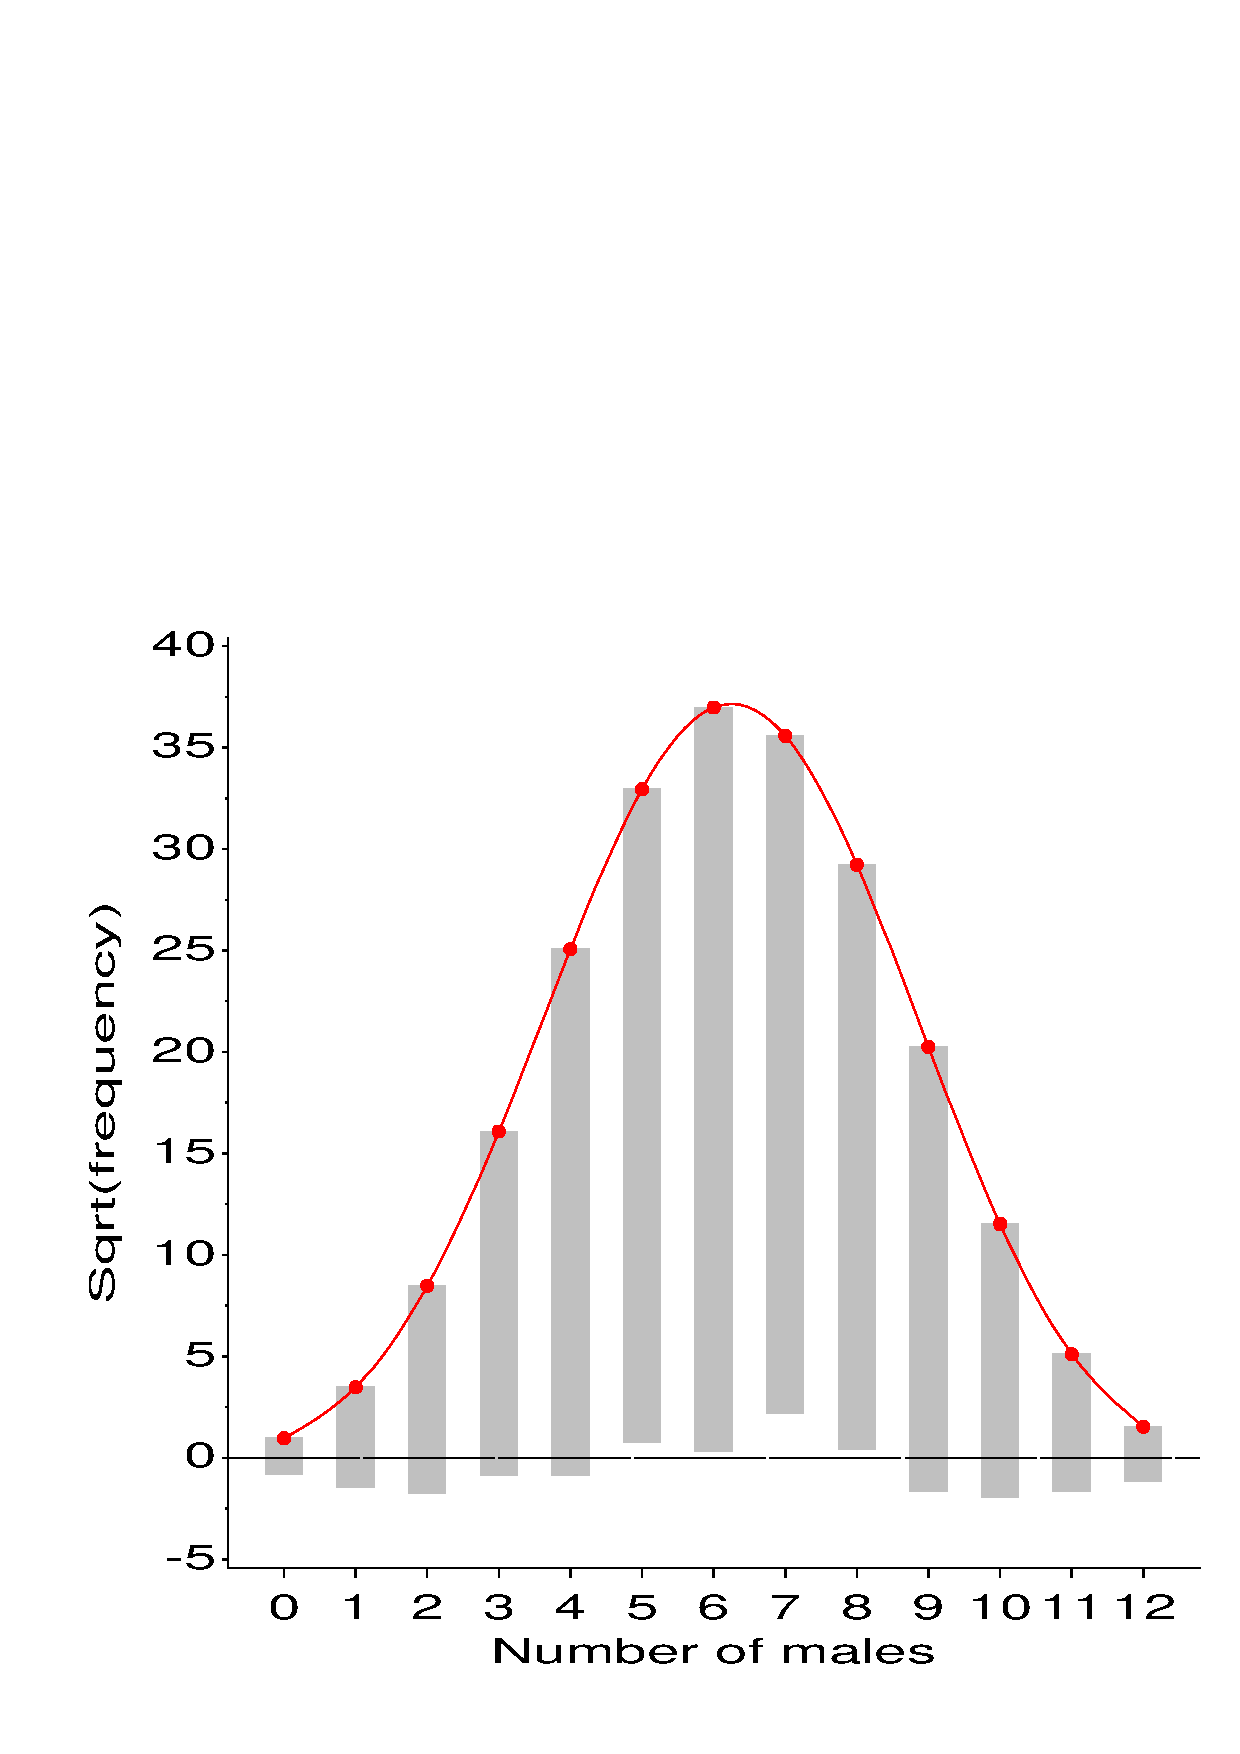
\includegraphics[width=1\linewidth]{saxony}\graphicsfile{ch2/fig/saxony.eps}{}
 \end{minipage}%
 \hfill
 \begin{minipage}[c]{.33\linewidth}
  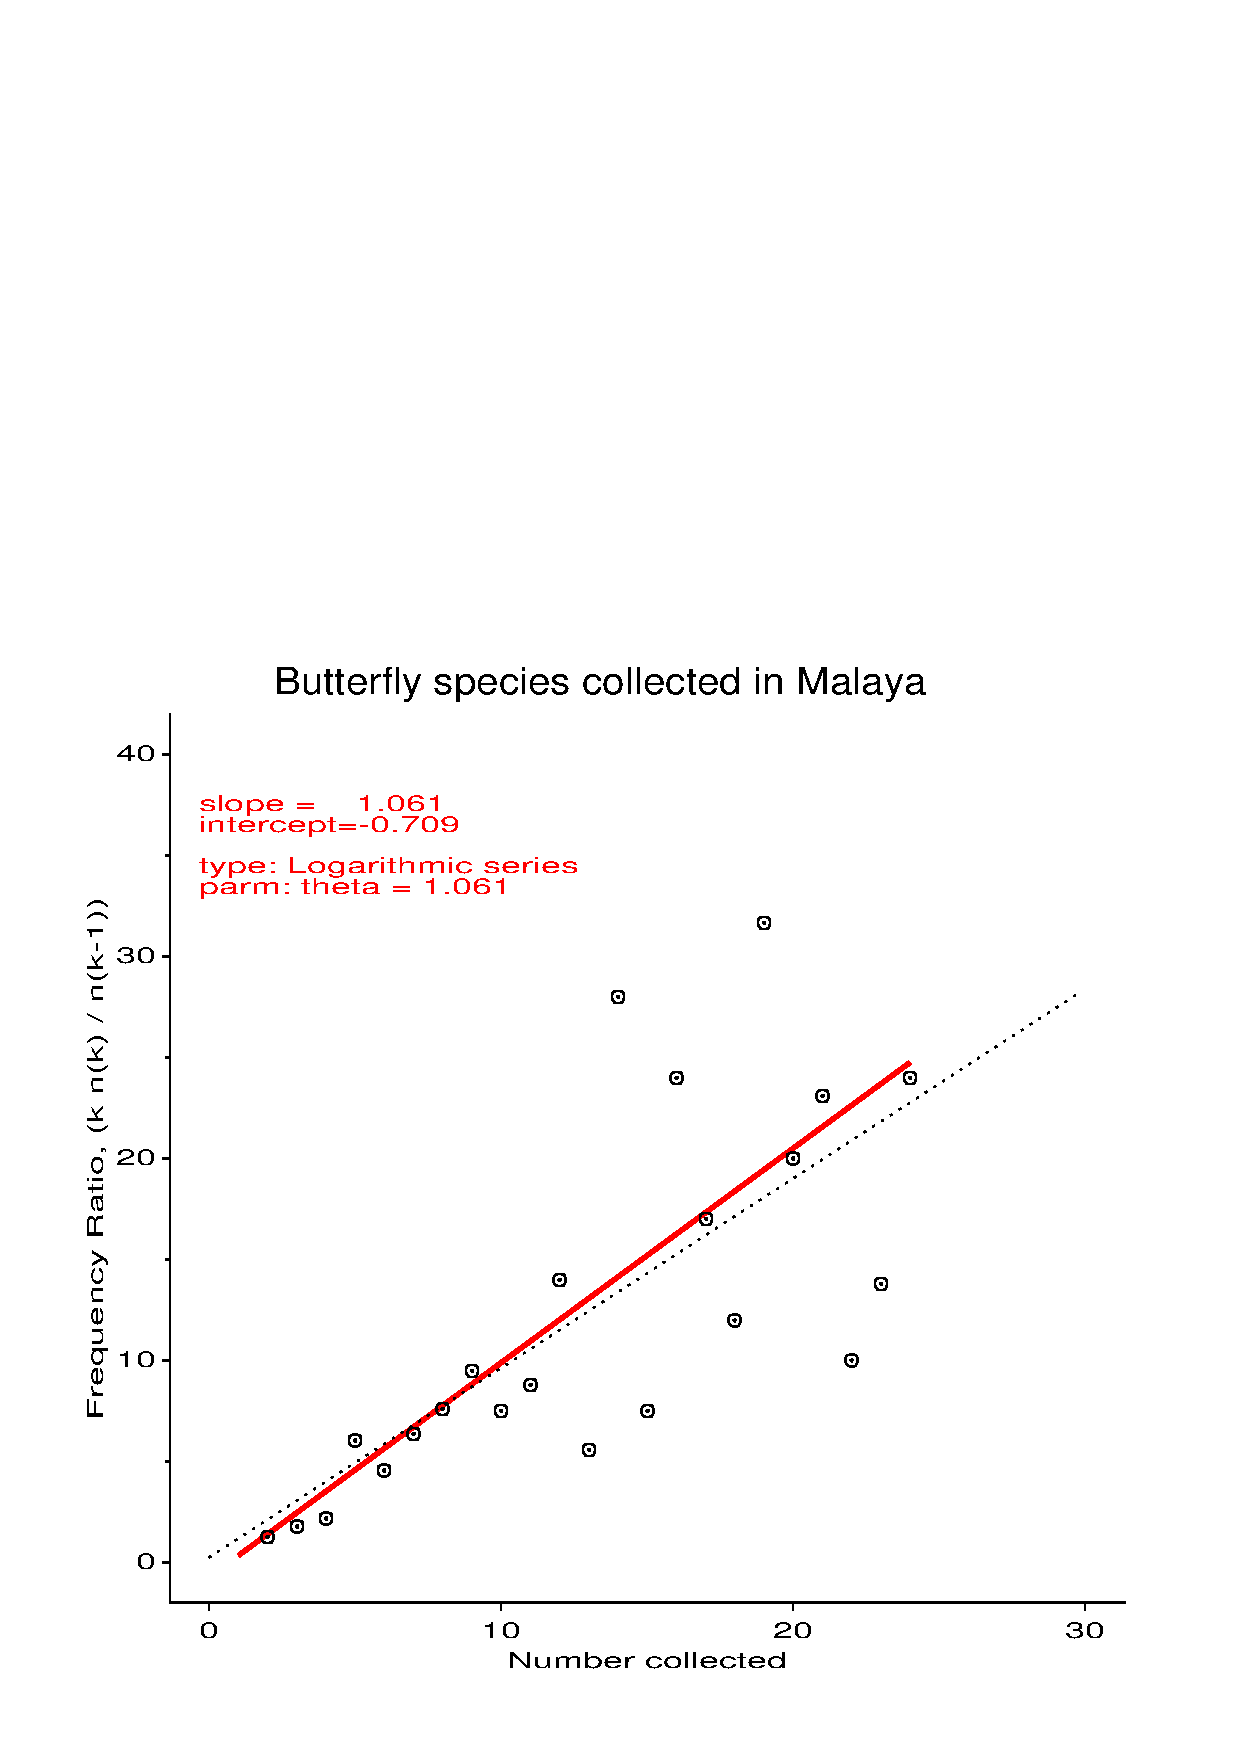
\includegraphics[width=1\linewidth]{orddemo3}\graphicsfile{ch2/fig/orddemo3.eps}{}
 \end{minipage}
 \hfill
 \begin{minipage}[c]{.33\linewidth}
  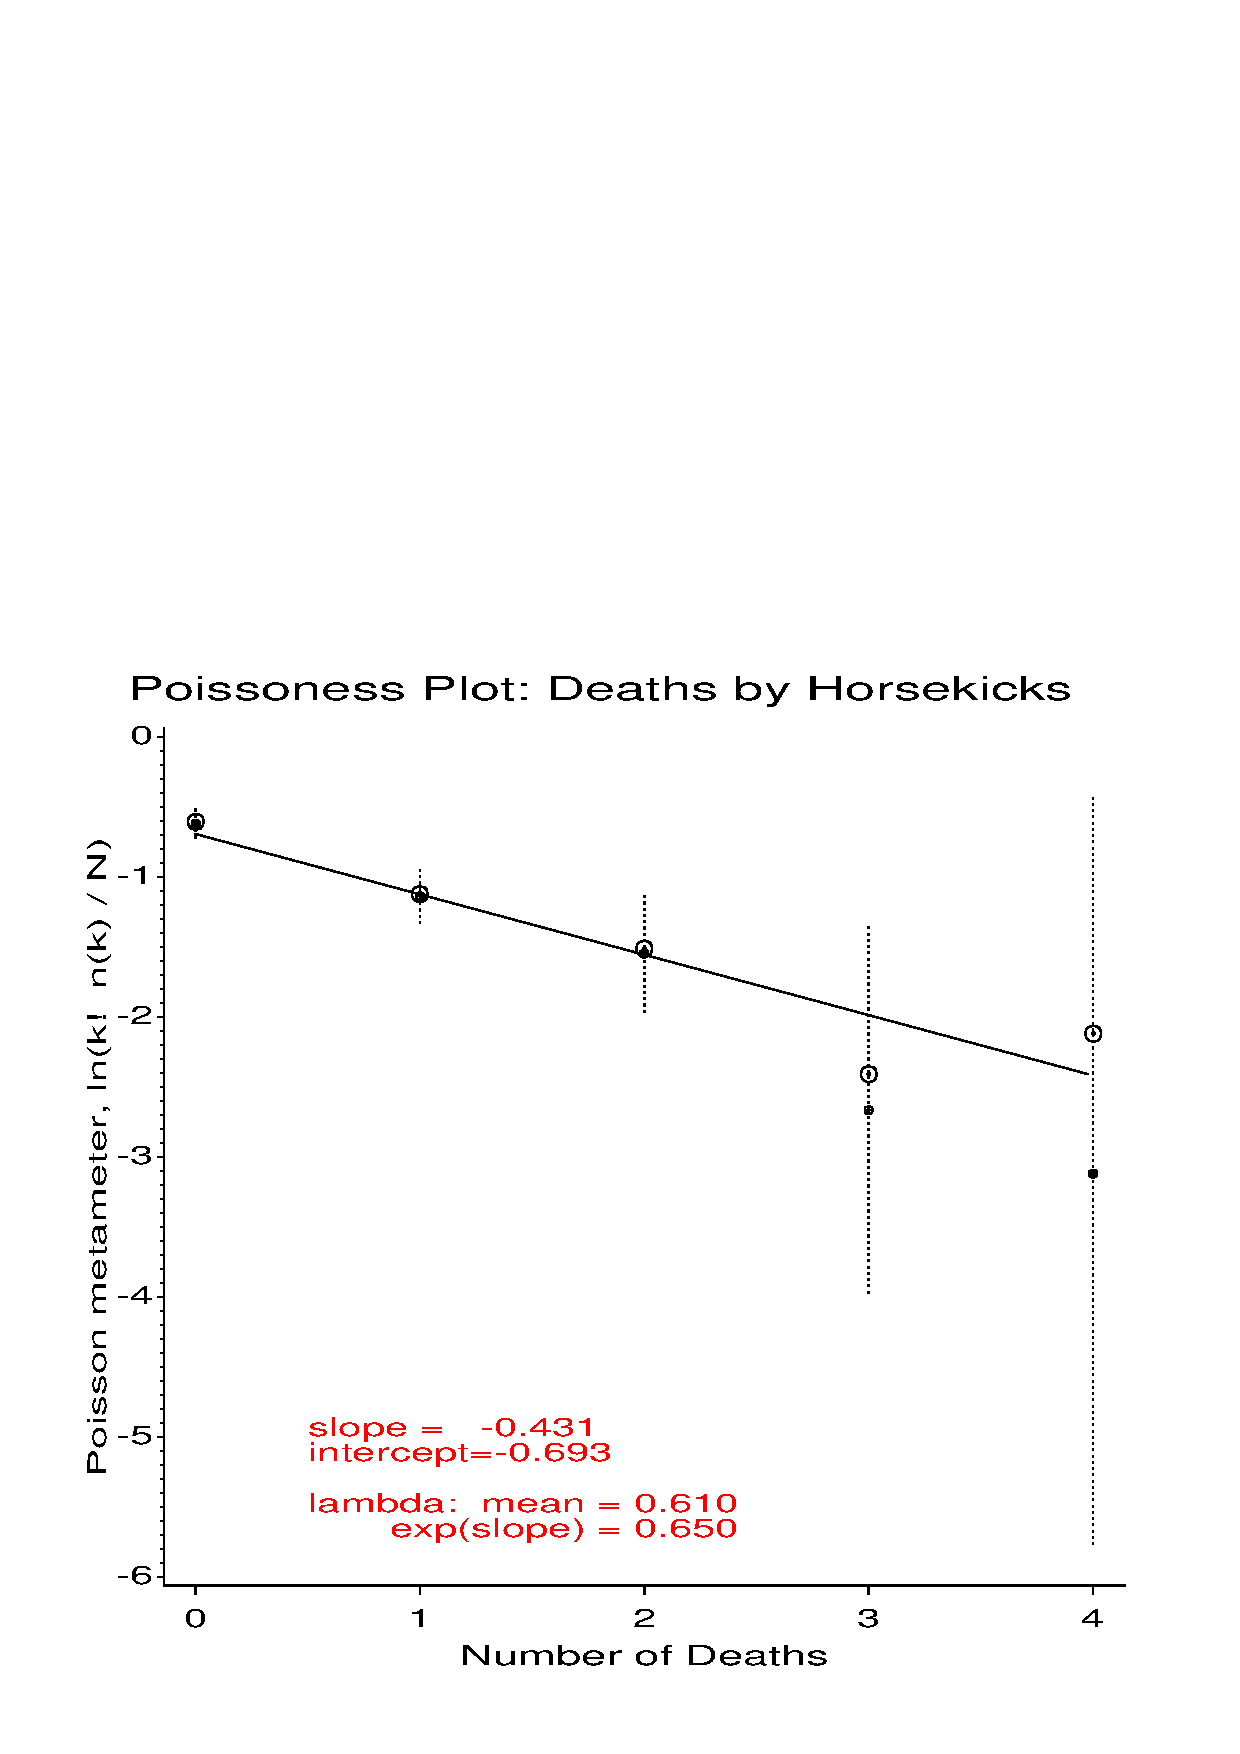
\includegraphics[width=1\linewidth]{poisdemo1}\graphicsfile{ch2/fig/poisdemo1.eps}{}
 \end{minipage}
\end{center}


\ixon{correspondence analysis}
\begin{quote}
{\Large
Correspondence analysis provides visualizations of associations in a two-way \ctab\
in a small number of dimensions.
Multiple correspondence analysis extends this technique to \nway\
tables.  Other grahical methods, including mosaic matrices and biplots
provide complementary views of \loglin\ models for two-way and \nway\
\ctab{}s.
}
\end{quote}
\minitoc
\clearpage

\section{Introduction}
\epigraph{Whenever a large sample of
chaotic elements
are taken in hand and marshaled in the order of their magnitude, an
unsuspected and most beautiful form of regularity proves to have been
latent all along.}
{Sir Francis Galton (1822-1911)}
Correspondence analysis (CA) is an exploratory technique which displays
the row and column categories in a two-way contingency table as points
in a graph, so that the positions of the points represent the
associations in the table.
Mathematically, correspondence analysis is related to the biplot,
to canonical correlation,
and to principal components analysis
(see \SSSGref{8,7, 9.4, 10.3}).
This technique finds
scores for the row and column categories on a small number of
dimensions which account for the greatest proportion of the
\(\chi^2\) for association between the row and column categories,
just as principal components account for maximum variance.
These scores provide a quantification of the categories,
and have the property that they maximize the correlation
between the row and column variables.   For
graphical display two or three dimensions are typically used to give
a reduced rank approximation to the data.

Correspondence analysis has a very large, multi-national literature and
was rediscovered several times in different fields and different countries.   The method, in slightly different forms, is also
discussed under the names
\boldital{dual scaling}, \boldital{optimal scaling},
\boldital{reciprocal averaging},
\boldital{homogeneity analysis},
and \boldital{canonical analysis of
categorical data}.

See \citet{Greenacre:84}, \citet{Nishisato:80},
or \citet{Gifi:81,Lebart-etal:77,Lebart-etal:84}
for a detailed treatment of the method and its applications.
\citet{GreenacreHastie:87} provide an excellent discussion of
the geometric interpretation,
while \citet{HeijdenLeeuw:85} and \citet{Heijden-etal:89}
develop some of the relations between correspondence analysis
and log-linear methods for three-way and larger tables.
Correspondence analysis is usually carried out in an exploratory,
graphical way; however,
\citet{Goodman:81,Goodman:85,Goodman:86} has developed related inferential models, the $RC$ model and
the canonical correlation model, with close links to \CA.

For a two-way table the scores for the row categories, namely
\(\mat{X} = \{x_{im}\}\), and column categories, \(\mat{Y} = \{y_{jm}\}\), on dimension \(m = 1,
\dots , \,  M\) are derived from a (generalized) singular value decomposition of
residuals from independence, expressed as \(d_{ij} /  \sqrt n\), to
account for the largest proportion of the \(\chi^2\) in a small
number of dimensions.  This decomposition may be expressed as
\ix{singular value decomposition}
%
\begin{equation} \label{eq:cadij}
  \frac{d_{ij}}{\sqrt{n}} = 
  \frac{n_{ij} - m_{ij}} {\sqrt {n \,  m_{ij}}} =
  \sum_{m=1}^M  \lambda_m \,  x_{im} \,  y_{jm}
  \comma
\end{equation}
where \(\lambda_1 \geq \lambda_2 \geq \cdots \geq \lambda_M\), and \(M
=  \min ( I-1 , \,  J-1 )\).  In \(M\) dimensions, the decomposition
\eqref{eq:cadij} is exact.
For example, an \(I \times 3\) table can be depicted exactly
in two dimensions when $I \ge 3$.  A rank-\(d\) approximation in \(d\) dimensions is
obtained from the first \(d\) terms on the right side of \eqref{eq:cadij};
the proportion of the Pearson \(\chi^2\) accounted for by this approximation is
\begin{equation*}
 n \,  \sum_m^d { \,  \lambda_m^2 } \big/  \chi^2
 \period
\end{equation*}
The quantity $\chi^2 /n = \sum_i \sum_j d_{ij}^2  / n$ is called
the total \glossterm{inertia} and is identical to the measure of
association known as Pearson's mean-square contingency, the
square of the $\phi$ coefficient.
\ix{$\phi$ coefficient}
\ix{phi coefficient@phi ($\phi$) coefficient}
\ix{mean-square contingency coefficient}

Thus, correspondence analysis is designed to show how the data
deviate from expectation when the row and column variables are
independent, as in the association plot and mosaic display.  However,
the association plot and mosaic display depict every \emph{cell} in
the table, and for large tables it may be difficult to see patterns.
Correspondence analysis shows only row and column \emph{categories} in
the two (or three) dimensions which account for the greatest
proportion of deviation from independence.
The pattern of the associations is inferred from the positions of the
row and column points.

\section{Simple correspondence analysis}\label{sec:ca-simple}
\ixon{correspondence analysis!two-way tables}
\subsection{Notation and terminology}\label{sec:ca-notation}
Because \CA\ grew up in so many homes, the notation, formulae
and terms used to describe the method vary considerably.
The notation used here generally follows \citet{Greenacre:84,Greenacre:97},
as does the documentation in the \STUGref{19}{The CORRESP Procedure}.

The descriptions here employ the following matrix and vector definitions:
\begin{itemize}
\item $\mat{N} = \{ n_{ij} \}$ is the $I \times J$ contingency table
with row and column totals $n_{i+}$ and $n_{+j}$, respectively.
The grand total $n_{++}$ is also denoted by $n$ for simplicity.
\item $\mat{P} = \{ p_{ij} \} = \mat{N}/n$ is the matrix of joint cell
probabilities,  called the \glossterm{correspondence matrix}.
\item $\vec{r} = \sum_j p_{ij} = \mat{P} \vec{1}$ is the row margin of $\mat{P}$;
$\vec{c} = \sum_i p_{ij} = \mat{P}\trans \vec{1}$ is the column margin.
$\vec{r}$ and $\vec{c}$ are called the \emph{row masses} and \emph{column masses}.
\item $\mat{D}_r$ and $\mat{D}_c$ are diagonal matrices with $\vec{r}$
and $\vec{c}$ on their diagonals, used as weights.
\item $\mat{R} = \mat{D}_r^{-1} \mat{P} = \{ n_{ij} / n_{+j} \}$ is the matrix of
row conditional probabilities, called \emph{row profiles}.
Similarly, $\mat{C} = \mat{D}_c^{-1} \mat{P}\trans = \{ n_{ij} / n_{i+} \}$ is the matrix of
column conditional probabilities or \emph{column profiles}.
\end{itemize}

Two types of coordinates, $X$, $Y$ for the row and column categories are defined,
based on the generalized singular value decomposition of $\mat{P}$,
\ix{singular value decomposition}
\begin{equation*}%\label{eq:ca-svd}
\mat{P} = \mat{A} \mat{D}_{\lambda} \mat{B}\trans
\end{equation*}
where $\mat{D}_{\lambda}$ is the diagonal matrix of singular values
\(\lambda_1 \geq \lambda_2 \geq \cdots \geq \lambda_M\),
$\mat{A}$ is the $I \times M$ matrix of left singular vectors,
normalized so that
\( \mat{A} \mat{D}_r^{-1} \mat{A}\trans = \mat{I} \), and
$\mat{B}$ is the $J \times M$ matrix of right singular vectors,
normalized so that
\( \mat{B} \mat{D}_c^{-1} \mat{B}\trans = \mat{I} \).
Thus the columns of $\mat{A}$ and $\mat{B}$ are orthogonal in the weighted metrics
defined by the row and column margins, $\mat{D}_r^{-1}$ and $\mat{D}_c^{-1}$,
respectively.
\begin{description}
\ix{correspondence analysis!principal coordinates}
\ix{principal coordinates}
\item[principal coordinates]  The coordinates of the row ($\mat{F}$) and column ($\mat{G}$) profiles
with respect to their own principal axes are defined so that the inertia along
each axis is the corresponding singular value, $\lambda_i$,
\begin{eqnarray}
%
\mat{F} & = & \mat{D}_r^{-1} \mat{A} \mat{D}_{\lambda} \quad\mbox{so that} \quad \mat{F}\trans \mat{D}_r \mat{F} = \mat{D}_{\lambda} \label{eq:pcoord1} \\
\mat{G} & = & \mat{D}_c^{-1} \mat{B} \mat{D}_{\lambda} \quad\mbox{so that} \quad \mat{G}\trans \mat{D}_c \mat{G} = \mat{D}_{\lambda} \label{eq:pcoord2}
\end{eqnarray}
\ix{correspondence analysis!standard coordinates}
\ix{standard coordinates}
\item[standard coordinates] The standard coordinates ($\mat{\Phi}, \mat{\Gamma}$) are a rescaling of the principal
coordinates to unit inertia along each axis,
\begin{eqnarray}
%\label{}
\mat{\Phi} & = & \mat{D}_r^{-1} \mat{A}  \quad\mbox{so that} \quad \mat{\Phi}\trans \mat{D}_r \mat{\Phi} = \mat{I} \\
\mat{\Gamma} & = & \mat{D}_c^{-1} \mat{B} \quad\mbox{so that} \quad \mat{\Gamma}\trans \mat{D}_c \mat{\Gamma} = \mat{I}
\end{eqnarray}
These differ from the principal coordinates in \eqref{eq:pcoord1}
and \eqref{eq:pcoord2} simply by the absence of the scaling factors,
$\mat{D}_{\lambda}$.
\end{description}
Thus, the weighted average of the squared principal coordinates
for the rows or columns on a principal axis equals the squared
singular value, $\lambda$ for that axis,
whereas the weighted average of the squared standard coordinates
equals 1.
The relative positions of the row or column points along any axis
is the same under either scaling,
but the distances between points differ, because the axes are
weighted differentially in the two scalings.


\subsection{Geometric and statistical properties}\label{sec:ca-properties}
\ixon{correspondence analysis!properties}
We summarize here some geometric and statistical properties of the
\CA\ solutions which are useful in interpretation.

\begin{description}
\item[nested solutions:] Because they use successive terms of the SVD
  \eqref{eq:cadij}, \CA\ solutions are \emph{nested}, meaning that the first
  two dimensions of a three-dimensional solution will be identical
  to the two-dimensional solution.

\item[centroids at the origin:] In both principal coordinates and standard
coordinates the points representing the row and column profiles have their
centroids (weighted averages) at the origin.
Thus, in \CA\ plots, the origin represents the (weighted) average
row profile and column profile.

\item[reciprocal averages:]
The column scores are proportional to the weighted averages of the row
scores, and vice-versa.

\item[chi-square distances:]  In principal coordinates, the row coordinates
may be shown equal to the row profiles $\mat{D}_r^{-1} \mat{P}$, rescaled inversely by the square-root of the column masses, $\mat{D}_c^{-1/2}$.
Distances between two row profiles, $\mat{R}_i$ and $\mat{R}_{i^\prime}$
is most sensibly defined as $\chi^2$ distances, where the squared
difference $[\mat{R}_{ij} -\mat{R}_{i^\prime j}]^2$ is inversely weighted
by the column frequency, to account for the different relative
frequency of the column categories.
The rescaling by $\mat{D}_c^{-1/2}$ transforms this weighted $\chi^2$
metric into ordinary Euclidean distance.
The same is true of the column principal coordinates.

\item[interpretation of distances:]
In principal coordinates,
the distance between two row points may be interpreted as described
above, and so may the distance between two column points.
The distance between a row and column point, however, does not have
a clear distance interpretation.

\item[residuals from independence:]
The distance between a row and column point do have a rough
interpretation in terms of residuals or the difference between
observed and expected frequencies, $n_{ij} - m_{ij}$.
Two row (or column) points deviate from the origin (the average
profile) when their profile frequencies have similar values.
A row point appears near a column point when  $n_{ij} - m_{ij} >
0$, and away from that column point when the residual is negative.
\end{description}

Because of these differences in interpretations of distances, there
are different possibilities for graphical display.
A joint display of principal coordinates for the rows and standard
coordinates for the columns (or vice-versa), sometimes called
an \emph{asymmetric map} is suggested by
\ix{correspondence analysis!asymmetric map}
\citet{GreenacreHastie:87} and by \citet{Greenacre:89} as the plot
with the most coherent geometric interpretation
(for the points in principal coordinates) and is widely
used in the French literature.
The options \pname{PROFILE=ROW} and \pname{PROFILE=COLUMN}
in \PROC{CORRESP} generate the asymmetric map.

\ix{correspondence analysis!symmetric map}
Another common joint display is the \emph{symmetric map} of the principal
coordinates in the same plot, produced with the option \pname{PROFILE=BOTH}.
In the author's opinion, this produces better graphical displays, because
both sets of coordinates are scaled with the same weights for each axis.
Symmetric plots are used exclusively in this book, but that should
not imply that these plots are universally preferred.
Another popular choice is to avoid the possibility of misinterpretation
by making separate plots of the row and column coordinates.
The different scalings, and the valid distance interpretations for each
are described in detail in the Algorithms section of
\STUGref{19}{The CORRESP Procedure}.
\ixoff{correspondence analysis!properties}

\subsection{The CORRESP Procedure}\label{sec:corresp}

Correspondence analysis is performed using \PROC{CORRESP} in \SSTAT.
\PROC{CORRESP} can read two kinds of input:

\begin{itemize*}
\item a two-way contingency table (\emph{contingency table form}),
where the columns are \Dset{}
variables (specified in a \stmt{var}{CORRESP}), and the rows are observations, labeled by an
\pname{id} variable.
In this case the column variables contain the frequencies in the
corresponding cells.
\ix{case form}
\ix{frequency form}
\item raw category responses (\emph{case form}), or cell frequencies (\emph{frequency
form}),
classified by two (or more) table variables.  In these two cases, the table variables are specified in
a \stmt{TABLES}{CORRESP}.  When the observations are cell frequencies,
the frequency variable may be specified in the \stmt{WEIGHT}{CORRESP}.
\end{itemize*}

In addition to printed output, the \opt{OUTC=}{CORRESP} produces an \ODS\
which contains the row and column
coordinates and other information.
To understand the relationships among the row and column categories
we may plot the coordinates with
\PROC{PLOT} or \PROC{GPLOT}.  The
procedure has many options for scaling row and column coordinates,
and for printing various statistics which aid interpretation.
We first illustrate the basic use of the procedure.
A macro program \pname{CORRESP} described in \secref{sec:ca-camacro}
simplifies the analysis and plotting steps.

\begin{Example}[haireye3]{Hair color and eye color}

The program below reads the hair and eye color data into the \Dset\
\pname{HAIREYE}, and calls the \proc{CORRESP}.  This example illustrates
the use of \PROC{PLOT} and the Annotate facility with \PROC{GPLOT} to
produce a labeled display of the correspondence analysis solution.
To input a contingency table in the CORRESP step, the hair colors
(columns) are specified as the variables in the \stmt{VAR}{CORRESP}, and
the eye colors (rows) are indicated as the ID variable.
%% \inclsas{corresp3)
%% input: /users/faculty/friendly/sasuser/catdata/corresp3.sas
%% last modified: 28-Jul-98 17:26
\begin{listing}
data haireye;
   input  EYE $ BLACK BROWN RED BLOND ;
datalines;
         Brown    68   119    26     7    
         Blue     20    84    17    94    
         Hazel    15    54    14    10    
         Green     5    29    14    16    
;
proc corresp data=haireye outc=coord short;
    var black brown red blond;
    id eye;
proc print data=coord;
   var _type_ eye dim1 dim2 quality;
\end{listing}

\ixd{hair-eye color}

The printed output from the \proc{CORRESP} is shown in
\outref{out:corresp3.1}.  The
section labeled ``Inertia and Chi-Square Decomposition'' indicates that over 98\% of the
Pearson
\(\chi^2\) for association is accounted for by two dimensions, with
most of that attributed to the first dimension.

\begin{Output}[htb]
\caption{Hair-eye data, \PROC{CORRESP} printed output}\label{out:corresp3.1}
\small
\verbatiminput{ch5/out/corresp3.1}
\end{Output}
\ixd{hair-eye color}

A plot of the row and column points can be constructed from the \pname{OUTC=}
\Dset\ \pname{COORD} requested in the \PROC{CORRESP} step.  The variables of
interest in this example are shown in \outref{out:corresp3.2}.  Note that row and
column points are distinguished by the variable \verb|_TYPE_|.
The labels for the points are stored in the \pname{id} variable,
\pname{eye} in this example.

\begin{Output}[htb]
\caption{Hair-eye data, OUTC=coord \Dset}\label{out:corresp3.2}
\small
\verbatiminput{ch5/out/corresp3.2}
\end{Output}
\ixd{hair-eye color}

The interpretation of the correspondence analysis results is
facilitated by a \emph{labeled} plot of the row and column points.
As of Version 6.08, points can be labeled in \PROC{PLOT}.  The
statements below produce a labeled plot.  The plot should be
scaled so that the number of data units/inch are the same for both
dimensions.  Otherwise, the distances (and angles) in this plot would not be
represented accurately.  In \PROC{PLOT}, this is done with the
\opt{VTOH}{PLOT}, which specifies the aspect ratio (vertical to
horizontal) of your printer, together with the \pname{HAXIS} and
\pname{VAXIS} options.

The \opt{VTOH}{PLOT} tries to equate distances between tick marks,  so you should
specify the same tick increment (e.g., \pname{HAXIS=BY xx}, \pname{VAXIS=BY xx}) for both axes.
For example, this \PROC{PLOT} step produces the
printer plot shown in \outref{out:corresp3.3}.
\ix{equating axes}

\begin{listing}
proc plot data-coord vtoh=2;
   plot dim2 * dim1 = '*'$ eye / box haxis=by .1 vaxis=by .1;
run;
\end{listing}

\begin{Output}[htb]
\caption{Labeled printer plot for the hair color, eye color \CA\ solution}\label{out:corresp3.3}
{\footnotesize
\begin{verbatim}
                 Plot of DIM2*DIM1$EYE.  Symbol used is '*'.
     -+----+----+----+----+----+----+----+----+----+----+----+----+----+----+-
DIM2 |                                                                       |
     |                                                                       |
 0.4 +                                                                       +
     |                                 * Green                               |
 0.3 +                   * RED                                               +
     |                                                                       |
 0.2 +                                                                       +
     |              * Hazel                                                  |
 0.1 +                                                                       +
     |                  * BROWN                                              |
 0.0 +                                                                       +
     |                                                             BLOND *   |
-0.1 +* Brown                                             * Blue             +
     |                                                                       |
-0.2 +* BLACK                                                                +
     |                                                                       |
-0.3 +                                                                       +
     |                                                                       |
     -+----+----+----+----+----+----+----+----+----+----+----+----+----+----+-
    -0.5 -0.4 -0.3 -0.2 -0.1  0.0  0.1  0.2  0.3  0.4  0.5  0.6  0.7  0.8  0.9
                                       DIM1
\end{verbatim}
}
\end{Output}
\ixd{hair-eye color}

A labeled high-resolution display of the correspondence analysis
solution (\figref{fig:corresp3}) is constructed with \PROC{GPLOT},
using a DATA step to produce an \ADS\ \pname{LABELS} from
the \pname{COORD} \Dset.  In the \PROC{GPLOT} step, axes are equated with
the AXIS statements: AXIS1 specifies a length and range which are
both twice that in the AXIS2 statement, so that the ratio of data
units to plot units is the same in both dimensions.
That is, the \pname{LENGTH} options are set so that
\ix{AXIS@\texttt{AXIS} statement!LENGTH@\texttt{LENGTH} option}
\ix{axes!equating}
\begin{equation*}
 \frac{ x_{\mbox{max}} - x_{\mbox{min}} } {  x_{\mbox{length}}} =
 \frac{ y_{\mbox{max}} - y_{\mbox{min}} } {  y_{\mbox{length}}}
 \period
\end{equation*}
Alternatively, you may use the \macro{EQUATE}
from the \SASSAMP\,
(see the \STUG\, Chapter 19, Example 3) 
which calculates the
desired lengths from the coordinates, or simply scale the aspect ratio
of the plot by using the options \texttt{HSIZE=} and \texttt{VSIZE=}
of the \texttt{GOPTIONS} statement.%
\footnote{The \texttt{HSIZE=} and \texttt{VSIZE=} options control the
entire plot size, including axis labels, titles and footnotes, so
setting these options, while easier, is less exact than setting the axis lengths.
}
The \macro{CORRESP}, illustrated in the next section, uses a version of the
\macro{EQUATE} (\macref{mac:equate}) modified to scale the plot automatically.
%% \inclsas{corresp3)
%% \input{corres3b} %% level: 3
%% input: /users/faculty/friendly/sasuser/catdata/corresp3.sas
%% last modified: 28-Jul-98 17:26
\begin{listing}
data label;
   set coord;
   xsys='2'; ysys='2';
   x = dim1; y = dim2;
   text = eye;
   size = 1.3;
   function='LABEL';
   if _type_='VAR' then color='RED  '; else color='BLUE'; 
data key;
    xsys='5'; ysys='5';
    length text $12;
    x = 25; y = 77;
    size = 1.4;
    color = 'BLUE ';
    function = 'LABEL   '; text = '* Eye color ' ; output;
    x = 55;
    color = 'RED  ';
    function = 'LABEL   '; text = '* HAIR COLOR' ; output;
data label;
    set key label;
proc gplot data=coord;
   plot dim2 * dim1
        / anno=label frame
          href=0 vref=0 lvref=3 lhref=3
          vaxis=axis2 haxis=axis1
          vminor=1 hminor=1;
   axis1 length=6 in  order=(-1. to 1. by .5)
         label=(h=1.5          'Dimension 1');
   axis2 length=3 in  order=(-.5 to .5 by .5)
         label=(h=1.5 a=90 r=0 'Dimension 2');
   symbol v=none;
run;
\end{listing}

\ixd{hair-eye color}

\begin{figure}[htb]
  \centering
  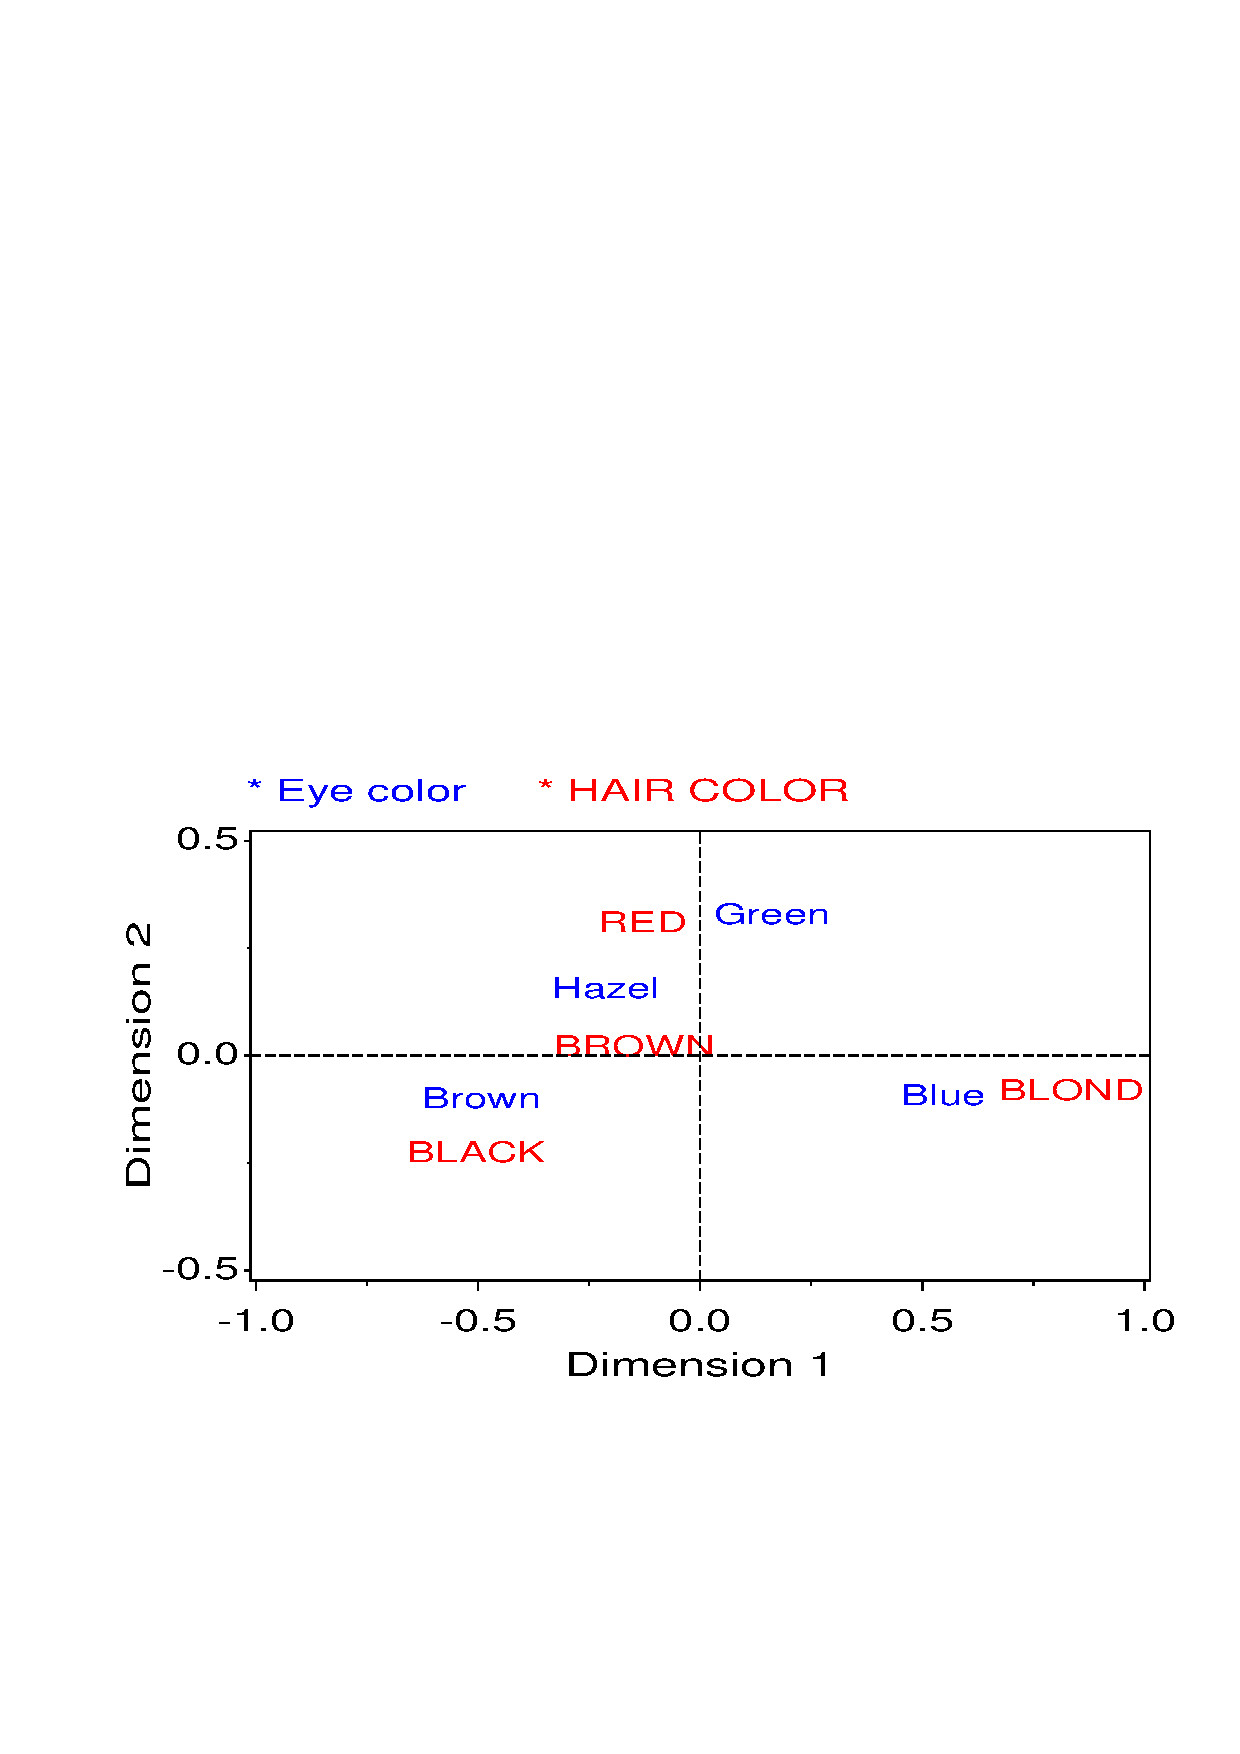
\includegraphics[scale=.7,clip=true]{ch5/fig/corresp3}
  \caption{Correspondence analysis solution for
Hair color, Eye color data}\label{fig:corresp3}
\end{figure}
\ixd{hair-eye color}
\end{Example}

\subsection{The \macro{CORRESP}}\label{sec:ca-camacro}

The steps illustrated in \exref{ex:haireye3} are not difficult, but it is somewhat tedious to do them repeatedly.
The \macro{CORRESP} (documented in \macref{mac:corresp})
is designed to make it easy to produce reasonable plots for \CA\
results.

The \macro{CORRESP}
\begin{itemize}
\item is designed as a simple macro interface to the \proc{CORRESP}.

\item It handles input in either contingency table form
(columns specified by the \mparm{VAR=}{CORRESP}, rows by the
\mparm{ID=}{CORRESP}), or frequency or case form 
(using the \mparm{TABLES=}{CORRESP}).

\item Three-way and larger tables may be analyzed by the ``stacking''
approach to
\mway\ tables described in \secref{sec:ca-multiway}, or by
the MCA approach.

\item Optionally, the macro produces a labeled printer plot and/or
\hires\ graphics plot, with many options for controlling the appearance
of graphics plots.
Axes for \hires\ plots may be equated automatically.
\item An \ODS\ containing the point coordinates and an \ADS\ containing point labels
are produced for further plotting or customization.
\end{itemize}

\begin{Example}[mental1]{Mental impairment and parents' SES}
\citet[p. 289]{Srole-etal:78} give the data below on the mental
health status of a sample of 1660 young New York residents in midtown Manhattan
classified by their parents' socioeconomic status (SES);
see \datref{dat:mental}.
There are five categories of SES and mental health is classified
in the four categories ``well'', ``mild symptom formation'',
``moderate symptom formation'', and ``impaired''.
These data have also been analyzed by many authors, including
\citet[ \S 8.5.2]{Agresti:90},
\citet{Goodman:79}, and
\citet[p. 375]{Haberman:79}.

The statements below read the data in contingency table form with rows identified
by the variable \pname{SES} and column variables \pname{well mild moderate impaired}.
These variables are used in the \verb|%CORRESP| call as the \pname{ID=}
and \pname{VAR=} parameters, respectively.
The graphics output is shown in \figref{fig:correses}.
\begin{figure}[htb]
  \centering
  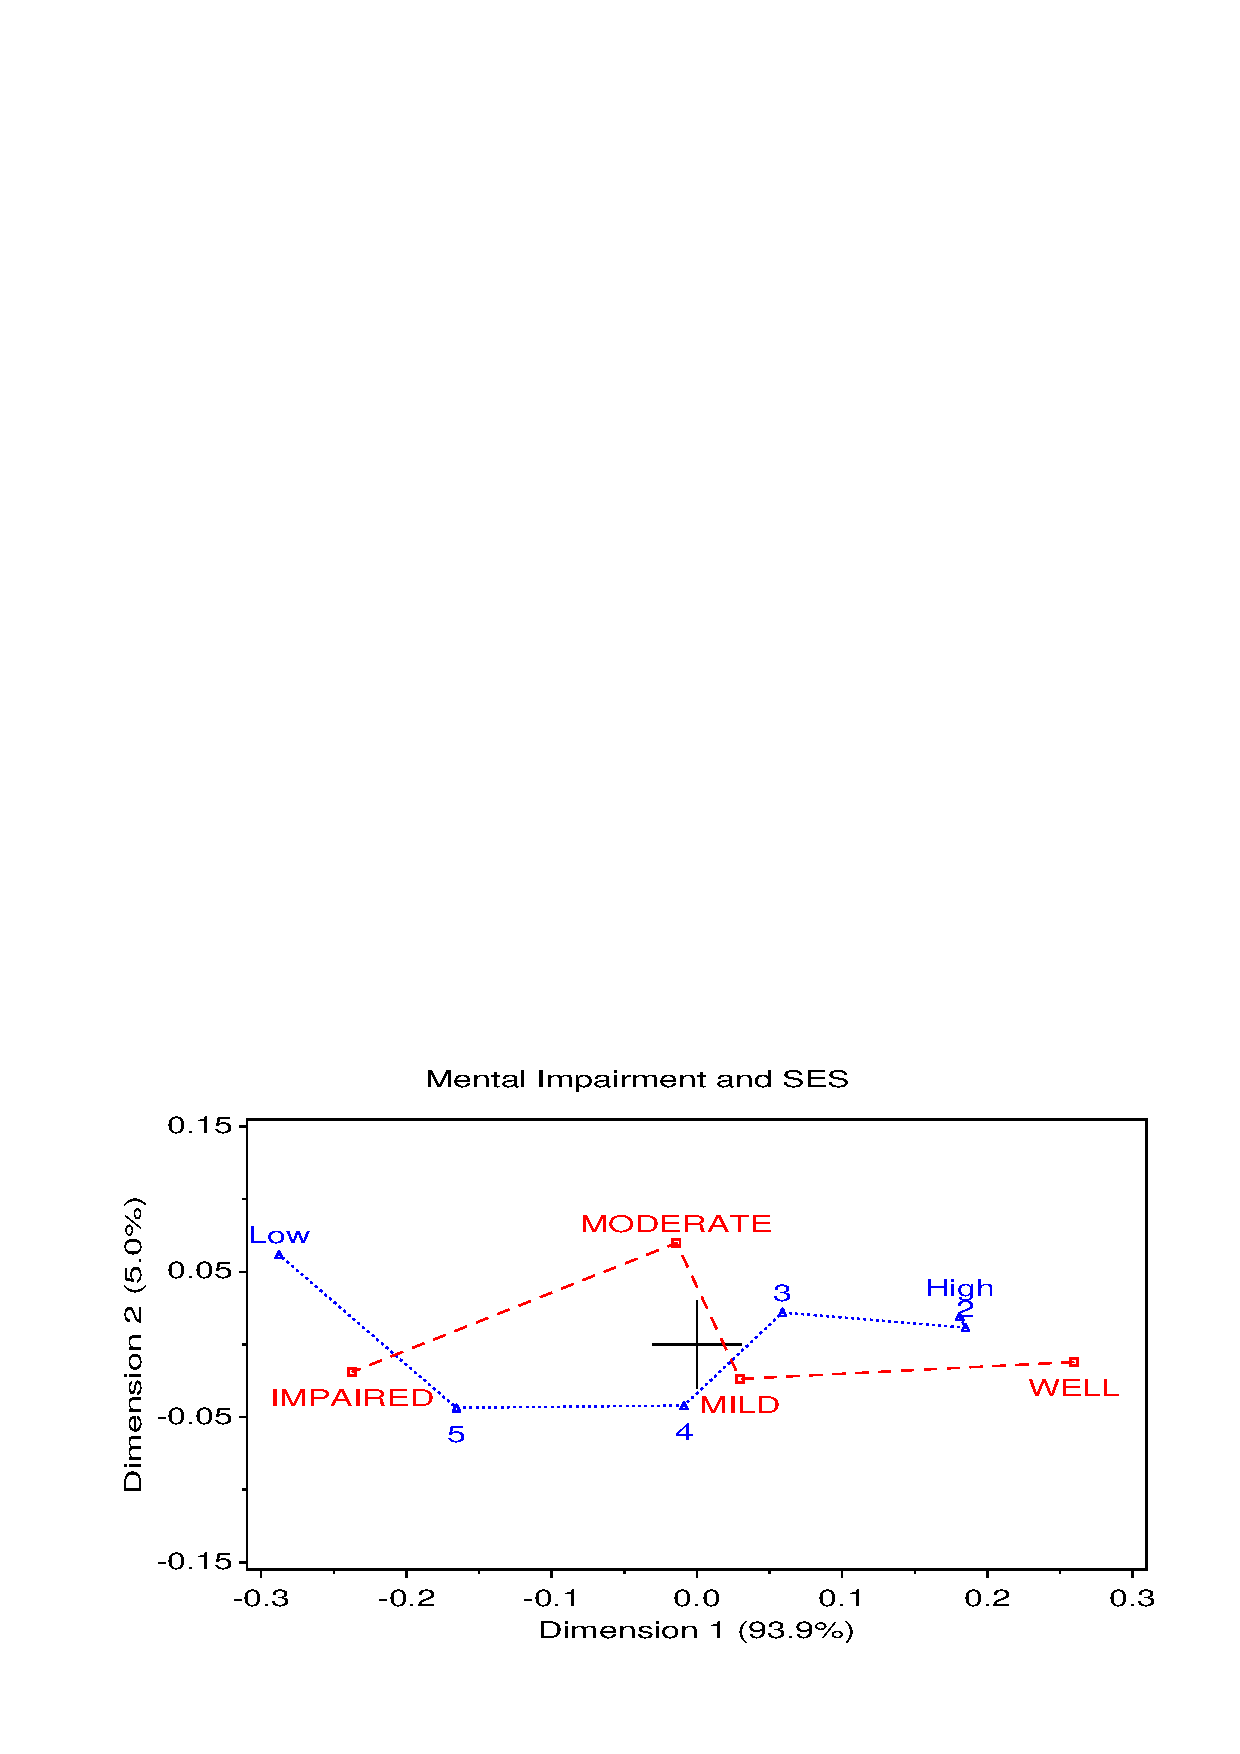
\includegraphics[scale=.8,clip=true]{ch\thechapter/fig/correses}
  \caption{\macro{CORRESP} plot for Mental Health data}\label{fig:correses}
\end{figure}
%% input: /Users/friendly/sasuser/catdata/correses.sas
%% last modified: 25-Jul-99  8:31
\begin{listing}
title h=1.5 lspace=3.8in 'Mental Impairment and SES';
data mental;
   input ses $ well mild moderate impaired;
datalines;
High 64     94     58     46
2    57     94     54     40
3    57    105     65     60
4    72    141     77     94
5    36     97     54     78
Low  21     71     54     71
;
axis1 length=3 in  order=(-.15 to .15 by .10)
      label=(h=1.5 a=90 r=0);
axis2 length=6 in  order=(-.30 to .30 by .10)
      label=(h=1.5) offset=(1);
%corresp (data=mental, id=ses, var=Well Mild Moderate Impaired,
      vaxis=axis1, haxis=axis2, htext=1.3, pos=-, interp=join,
      symbols=triangle square);
\end{listing}

Some of the graphics options for the \macro{CORRESP}
are illustrated by the \pname{htext=} (height of text labels),
\pname{pos=} (position of text labels), \pname{interp=} (point marker interpolation),
and \pname{symbols=} (point symbols) options.
In particular, the option \pname{pos=-} causes the macro to position the text labels
centered above or below the point depending on whether the $y$ position is positive
or negative
(as provided by the \macro{LABEL}; see \macref{mac:label}).

The cross at the origin in \figref{fig:correses} is drawn with equal data units in the
$x$ and $y$ direction, and so serves as a guide to whether the axes
have been equated.  The \pname{LENGTH} and \pname{ORDER} values on the \stmt{AXIS}{GPLOT}s
shown above
were determined by inspection after an initial plot.

We see from the plot that the association between mental health
and parents' SES is almost entirely 1-dimensional, with 94\% of
the \chisq\ ( 45.98, with 15 df) accounted for by Dimension 1.
The diagnostic categories are well-aligned with this dimension and
the two intermediate categories are closer on this dimension than
the extremes, indicating that their profiles differ little.  The
SES categories are also aligned with Dimension 1, and approximately
equally spaced, with the exception of the highest two categories.
Because both row and column categories have the same pattern on
Dimension 1, we may interpret the plot as showing that the profiles
of both variables are ordered, and their relation can be explained
as a positive association between parents' SES and higher mental
health status of children.

From a modeling perspective,  we might ask how strong is the evidence
for the spacing of categories noted above.  For example, we might
ask whether assigning integer scores to the levels of SES and mental
impairment provides a simpler, but satisfactory account of their association.
This question will be explored in a later chapter (see \exref{ex:mental2}).
\end{Example}

%% input: /users/faculty/friendly/sasuser/mosaics/victims.sas
%% last modified: 05-May-98 15:46
\begin{listing}
   *-- rearrange rows/cols by CA dim1;
   keep = \{2 3 1 5 4\};
   table = table[keep,keep];
   lnames = lnames[,keep];
 
   *-- standardize table to equal margins;
   avg = table[,+] / levels[1];
   newtab = repeat(avg,1,5);
   config = \{1 2\};
   call ipf(adjusted, status, levels, newtab, config, table);
   title  = 'Repeat Victimization Data, Adjusted to Equal Margins';
   lab = crime[keep];
   print title, adjusted[r=lab c=lab f=8.2];
   plots = 2;
   run mosaic(levels, adjusted, vnames, lnames, plots, title);

   *-- fit quasi-independence (ignore diagonal cells);
   title  = 'Repeat Victimization Data, Quasi Independence';
   zeros = J(5,5) - I(5);
   run mosaic(levels, adjusted, vnames, lnames, plots, title);
quit;
\end{listing}

\subsection{Quasi-independence and structural zeros}\label{sec:ca-quasi}
\ixon{quasi-independence}
\ixon{structural zeros}
\ixon{zeros!structural}
Incomplete tables can result when particular cells are simply not observed
(sampling zeros, e.g., insufficient data collected) or when some combinations of levels cannot logically occur (structural zeros, e.g., pregnant males).
Alternatively, in some cases we may wish to ignore the data in some cells,
and fit a quasi-independence model to the remaining cells. This is commonly
done with square tables having the same row and column categories,
where the dominant diagonal cells cause a global independence model to fail.

Because CA decomposes departures from independence,
many of these cases can be handled simply by estimating the expected
frequencies which would occur in these cells
if the row and column variables were
independent, and replacing the zero, missing, or dominant observed
frequencies by their expected values.%
\footnote{This does not, however, account properly for the loss in
degrees of freedom, but significance tests in CA are usually not
treated formally.
Indeed, the method would be of little interest for data in which
independence holds.}
More general, iterative procedures are discussed by \citet[\S 8.5]{Greenacre:84}
and by \citet[Ch. 3]{Heijden:87}.

\begin{Example}[victims3]{Repeat victimization}
\exref{ex:victims} also showed a mosaic display 
(\figref{fig:victims3}) for the model of quasi-independence
ignoring the diagonal cells in the repeat victimization data.
The analysis below gives another view of this model.

The elements in the diagonal cells of the \pname{VICTIMS} \Dset\
can be replaced by their expected frequencies under independence
in the following \IML\ step.
\begin{listing}
proc iml;
   use victims;
   read all var _num_  into table[r=crime c=vars];
   read all var {crime} into crime;
   close victims;

   exp = table[,+] * table[+,] / table[+,+];
   table = table + diag(vecdiag(exp - table));

   create victims from table[r=crime c=vars];
   append from table[r=crime c=vars];
\end{listing}
Using the same \verb|%CORRESP| step and plotting steps
as in \exref{ex:victims2} (with a different \stmt{LEGEND}{GPLOT})
gives the 2D plot shown in
\figref{fig:corresp5b}.

%% one figure
\begin{figure}[htb]
  \centering
  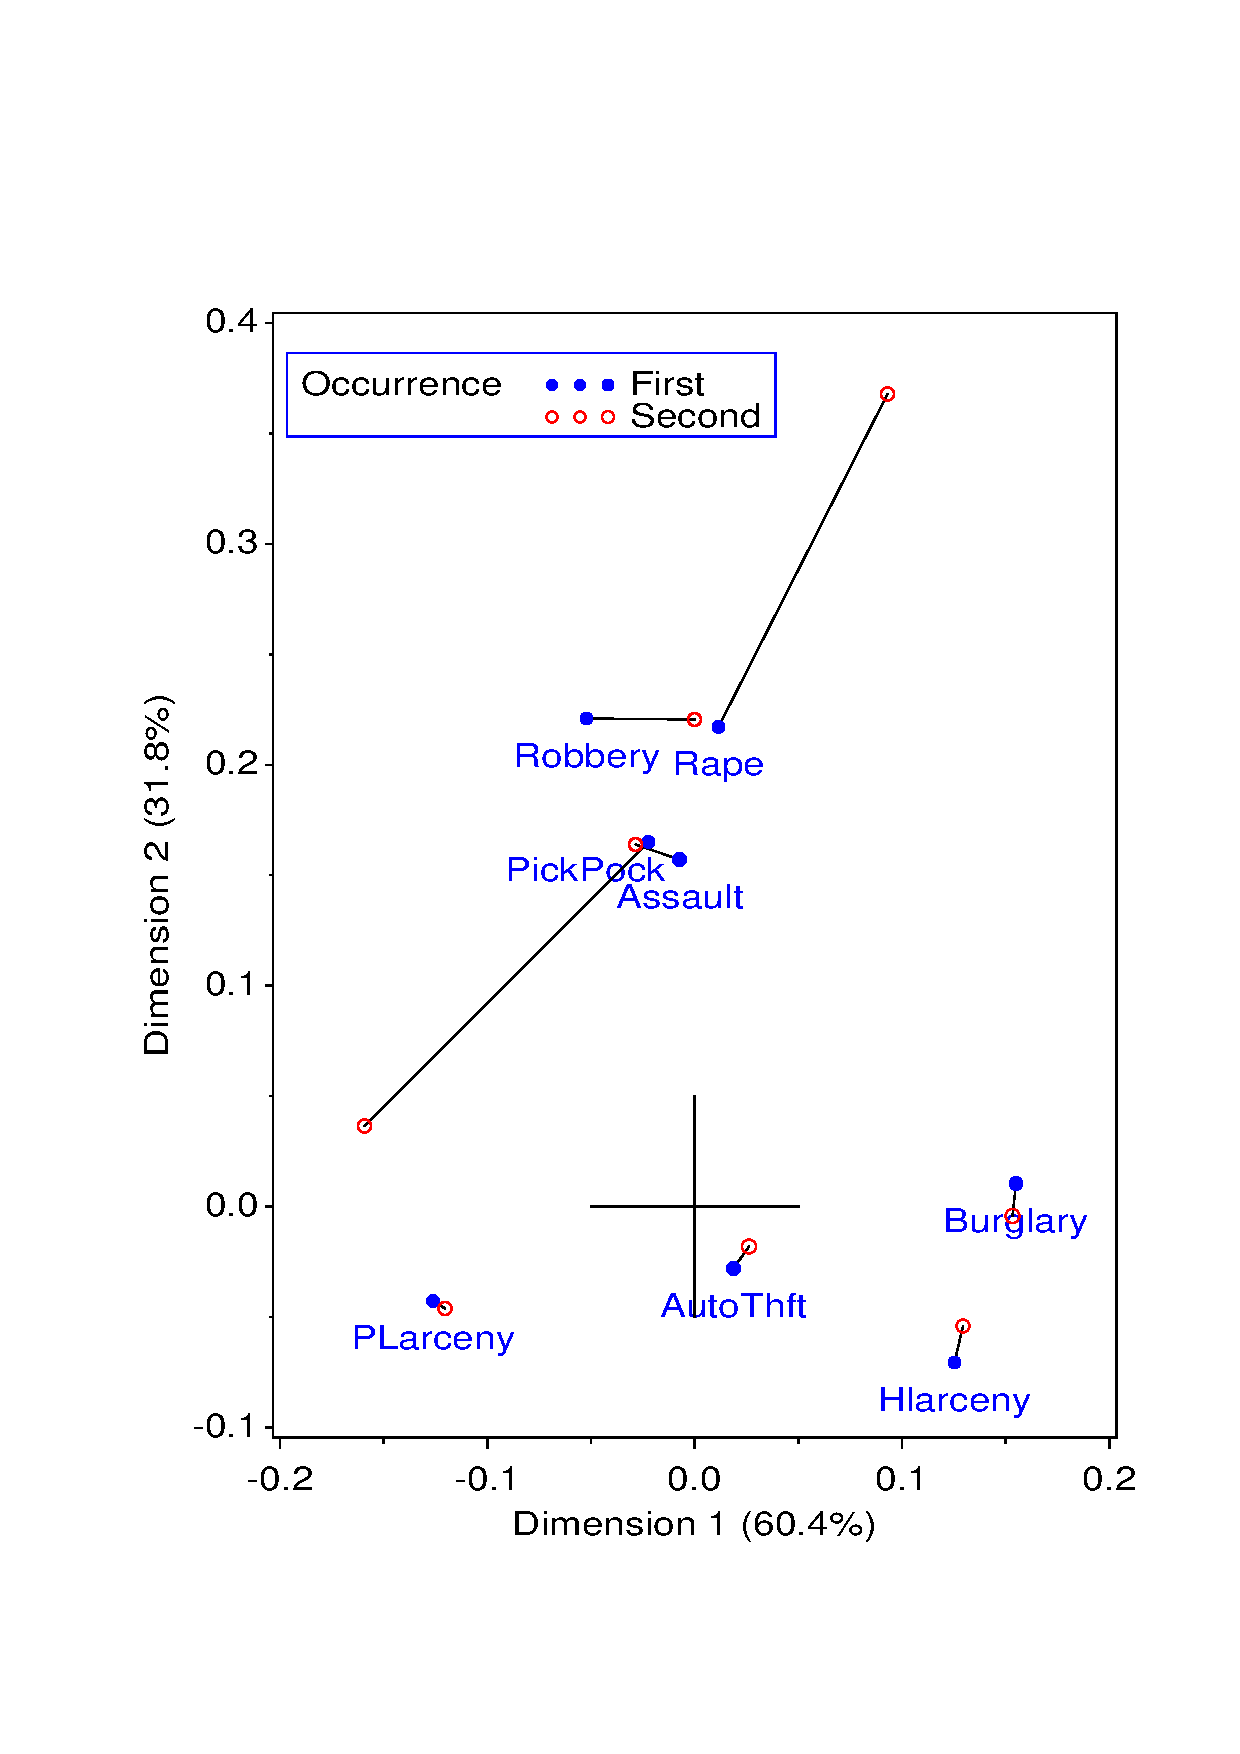
\includegraphics[scale=.6,clip]{ch5/fig/corresp5b}
  \caption[Repeat victimization data, quasi-independence
  model]{2D \CA\ display for repeat victimization data, quasi-independence
  model, ignoring diagonal cells.}%
  \label{fig:corresp5b}
\end{figure}
Note that the 2D solution now accounts for 92\% of the remaining
association, which now concerns only the cells where the crime differs
from first to second occurrence.
For these cells, the differences between first and second incident are
magnified.
\end{Example}
\ixoff{zeros!structural}
\ixoff{structural zeros}
\ixoff{quasi-independence}

\ixoff{correspondence analysis!two-way tables}
\section{Properties of category scores}
This section illustrates several properties of the \CA\
scores through calculation and visualization.

\subsection{Optimal category scores}\label{sec:scores}
The singular values shown in \outref{out:corresp3.1} are the \(\lambda_i\), in Eqn. \eqref{eq:cadij}.  They are also the
(canonical) correlations between the optimally scaled categories.
Thus, if the \pname{DIM1} scores for hair color and eye color are assigned to
the 592 observations in the table, the correlation of these variables
would be 0.4569 --- the largest possible correlation for \emph{any}
assignment of scores.
The \pname{DIM2} scores give a second, orthogonal scaling
of these two categorical variables, whose correlation would be
0.1491.

In this sense, CA scores provide an optimal way of transforming
categorical water into quantitative wine,  hence the name ``optimal
scaling''.

We can illustrate this numerically and visually
as follows. If the row scores on dimension 1 are
in the $r \times 1$ vector $\vec{x}_1$ and the column scores are in the
$c \times 1$ vector $\vec{y}_1$, then these scores can be expanded to
conform with the $r \times c$ table by forming the appropriate outer
product with a unit vector:
\begin{equation*}
 \mat{X}_1 = \vec{x}_1 \: \vec{1}\trans
 \qquad \mbox{and} \qquad
 \mat{Y}_1 = \vec{1} \: \vec{y}_1\trans
 \period
\end{equation*}

The program below uses \IML\ to perform this operation on the \pname{COORD}
\Dset\ and then merges these scores with a reshaped copy of the
\pname{haireye} data.
The resulting \Dset\ is shown in \outref{out:cascores.1}.

The \CA\ scores then serve to quantify the hair color and eye color
categories producing the maximal possible correlations of $(X1, Y1)$ and
$(X2, Y2)$, while all other pairs are uncorrelated.
These correlations are shown in \outref{out:cascores.2}.
A plot of the optimal scores, using cell frequencies as weights
(\figref{fig:cascores}) is developed in the next subsection.
%% input: /users/faculty/friendly/sasuser/catdata/cascores.sas
%% last modified: 29-Jul-98 15:28
\begin{listing}
*-- Attach X, Y values to eye color, hair color and reshape;
proc iml;
   use coord;
   read all var\{dim1 dim2\} where (_type_='VAR') into var[r=eye]; hair=eye;
   read all var\{dim1 dim2\} where (_type_='OBS') into obs[r=eye];
   
   r = nrow(obs);
   c = nrow(var);
   x1 = obs[,1] * j(1, c);
   x2 = obs[,2] * j(1, c);
   y1 = j(r,1)  * t(var[,1]);
   y2 = j(r,1)  * t(var[,2]);
   
   hair = repeat( hair, r, 1);
   eye  = shape(repeat( eye, 1,c),r*c, 1);

   create scores var\{eye hair x1 y1 x2 y2\};
   append;
   quit;

*-- Reshape data to frequency form and merge with scores;
proc transpose data=haireye out=haireye2;
   var BLACK BROWN RED BLOND;
   by eye notsorted;

data haireye2;
   set haireye2;
   rename _name_=hair col1=count;

data scores;
   merge haireye2 scores;

proc print data=scores;
   format x1 x2 y1 y2 7.4;
   id eye hair;

*-- Correlations of scores = singular values;
proc corr data=scores nosimple;
   freq count;
   var x1 x2;
   with y1 y2;   

\end{listing}


\begin{Output}[htb]
\caption{Hair-eye data, DIM1, DIM2 scores assigned to hair-eye categories}\label{out:cascores.1}
\small
\verbatiminput{ch5/out/cascores.1}
\end{Output}
\ixd{hair-eye color}

\begin{Output}[htb]
\caption{Hair-eye data, correlations between X1, X2 and Y1 Y2}\label{out:cascores.2}
\small
\verbatiminput{ch5/out/cascores.2}
\end{Output}
\ixd{hair-eye color}

\subsection{Simultaneous linear regressions}
The correlations among the \CA\ scores have yet another interpretation which gave
rise to the first algebraic derivation of the technique
\citep{Hirschfeld:35} and which today provides an important concept in the
\citet{Gifi:90} system of homogeneity analysis.

Consider an arbitrary assignment of scores $X1$ ($Y1$) to the hair color
(eye color) categories, for example $X1$ ($Y1$) = 1, 2, 3, 4 for the
categories in alphabetical order.
Instead of plotting these scores along a dimension as in \figref{fig:corresp3}, we plot $Y1$ against $X1$ for all $n = 592$
cases and show the frequency at each discrete point by the area of
a bubble symbol, as in \figref{fig:cascore0}.

\begin{figure}[htb]
  \centering
  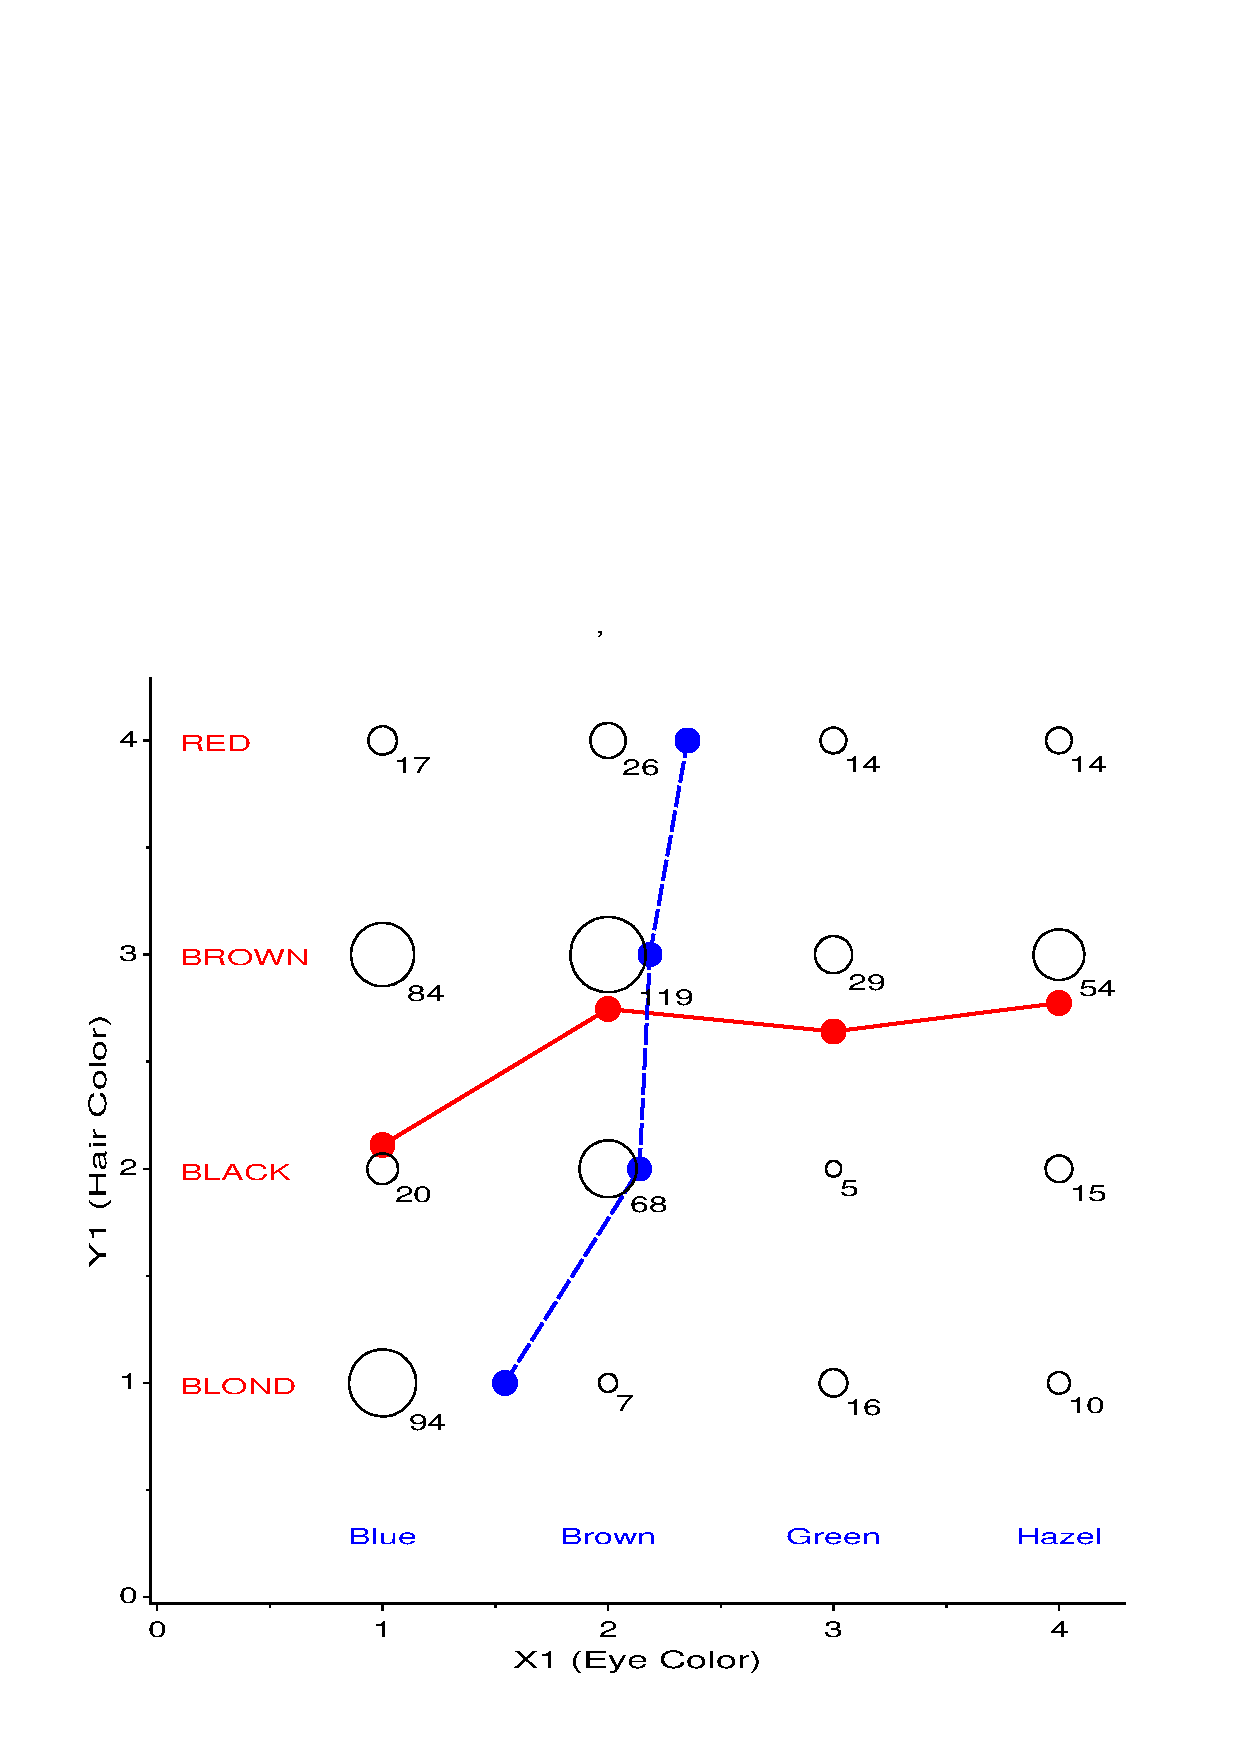
\includegraphics[scale=.6,clip]{ch5/fig/cascore0}
  \caption[Plot of arbitrary scores for the row and column categories]{Plot of arbitrary scores for the row and column categories.
The bubble symbols and numbers show the frequency at each point.
The red points (solid line) show the means of $Y1\given X1$; blue points (dashed line) show the means of $X1\given Y1$.}\label{fig:cascore0}
\end{figure}

If we carried out a least squares regression of  $Y1$ on $X1$,
this would be equivalent to finding the weighted mean of  $Y1$ for each value of $X1$ and fitting a straight line to these means.
Similarly, we could fit a regression of $X1$ on $Y1$,  which would be
determined by the weighted means of $X1$ for each $Y1$.
For the arbitrary scores, the conditional means of $Y1\given X1$
have a nonlinear relation to $X1$, and the same is true for the
inverse regression of $X1\given Y1$, as we see in \figref{fig:cascore0}.
The question posed by \citet{Hirschfeld:35} was this:
Can we find scores $\vec{a}$ and $\vec{b}$ for the row and column
variables such that \emph{both} regressions are linear?

The answer is ``Yes!''; indeed there is one solution for each pair of
\CA\ scores, $\vec{a}_i$ and $\vec{b}_i$, associated with the singular value $\lambda_i$.
For a given set of scores, $\vec{a}_i$ and $\vec{b}_i$, the weighted means
of the columns are
\(\mat{D}_c^{-1} \mat{P} \trans \vec{a}_i \), and the linear regression on
$\vec{b}_i$ has intercept 0 and slope $\lambda_i$,
\begin{equation*}%\label{eq:calin1}
(\mat{D}_c^{-1} \mat{P} \trans) \vec{a}_i = \lambda_i \vec{b}_i
\end{equation*}
Similarly, the inverse regression on $\vec{a}_i$ has intercept 0 and slope $1/\lambda_i$
\begin{equation*}%\label{eq:calin2}
(\mat{D}_r^{-1} \mat{P}) \vec{b}_i = (1/\lambda_i) \vec{a}_i
\end{equation*}
The choice of the scores associated with the largest singular value,
$\lambda_1$, makes the slope (equivalently, the correlation) of the
regression of $Y1$ on $X1$ as large as possible.
Moreover, this choice makes the angle between the two regression lines
as small as possible, i.e., the regressions are most collinear
\citep{Greenacre:84}.
So, instead of complex, nonlinear relations between the scaled
hair color and eye color variables using arbitrary scores (\figref{fig:cascore0}),
we arrive at simple, linear relations by use of a nonlinear
transformation of the arbitrary scores.

We can show these regressions for the first \CA\ dimension
in the following program steps, which continue from those
shown in \secref{sec:scores}.
Most of the program steps are concerned with finding the means
of $Y1\given X1$ and $X1\given Y1$, and annotating them on the
plot, together with the category labels and the regression line.
The plot with both regression lines is shown in \figref{fig:cascores}.
\begin{figure}[htb]
  \centering
  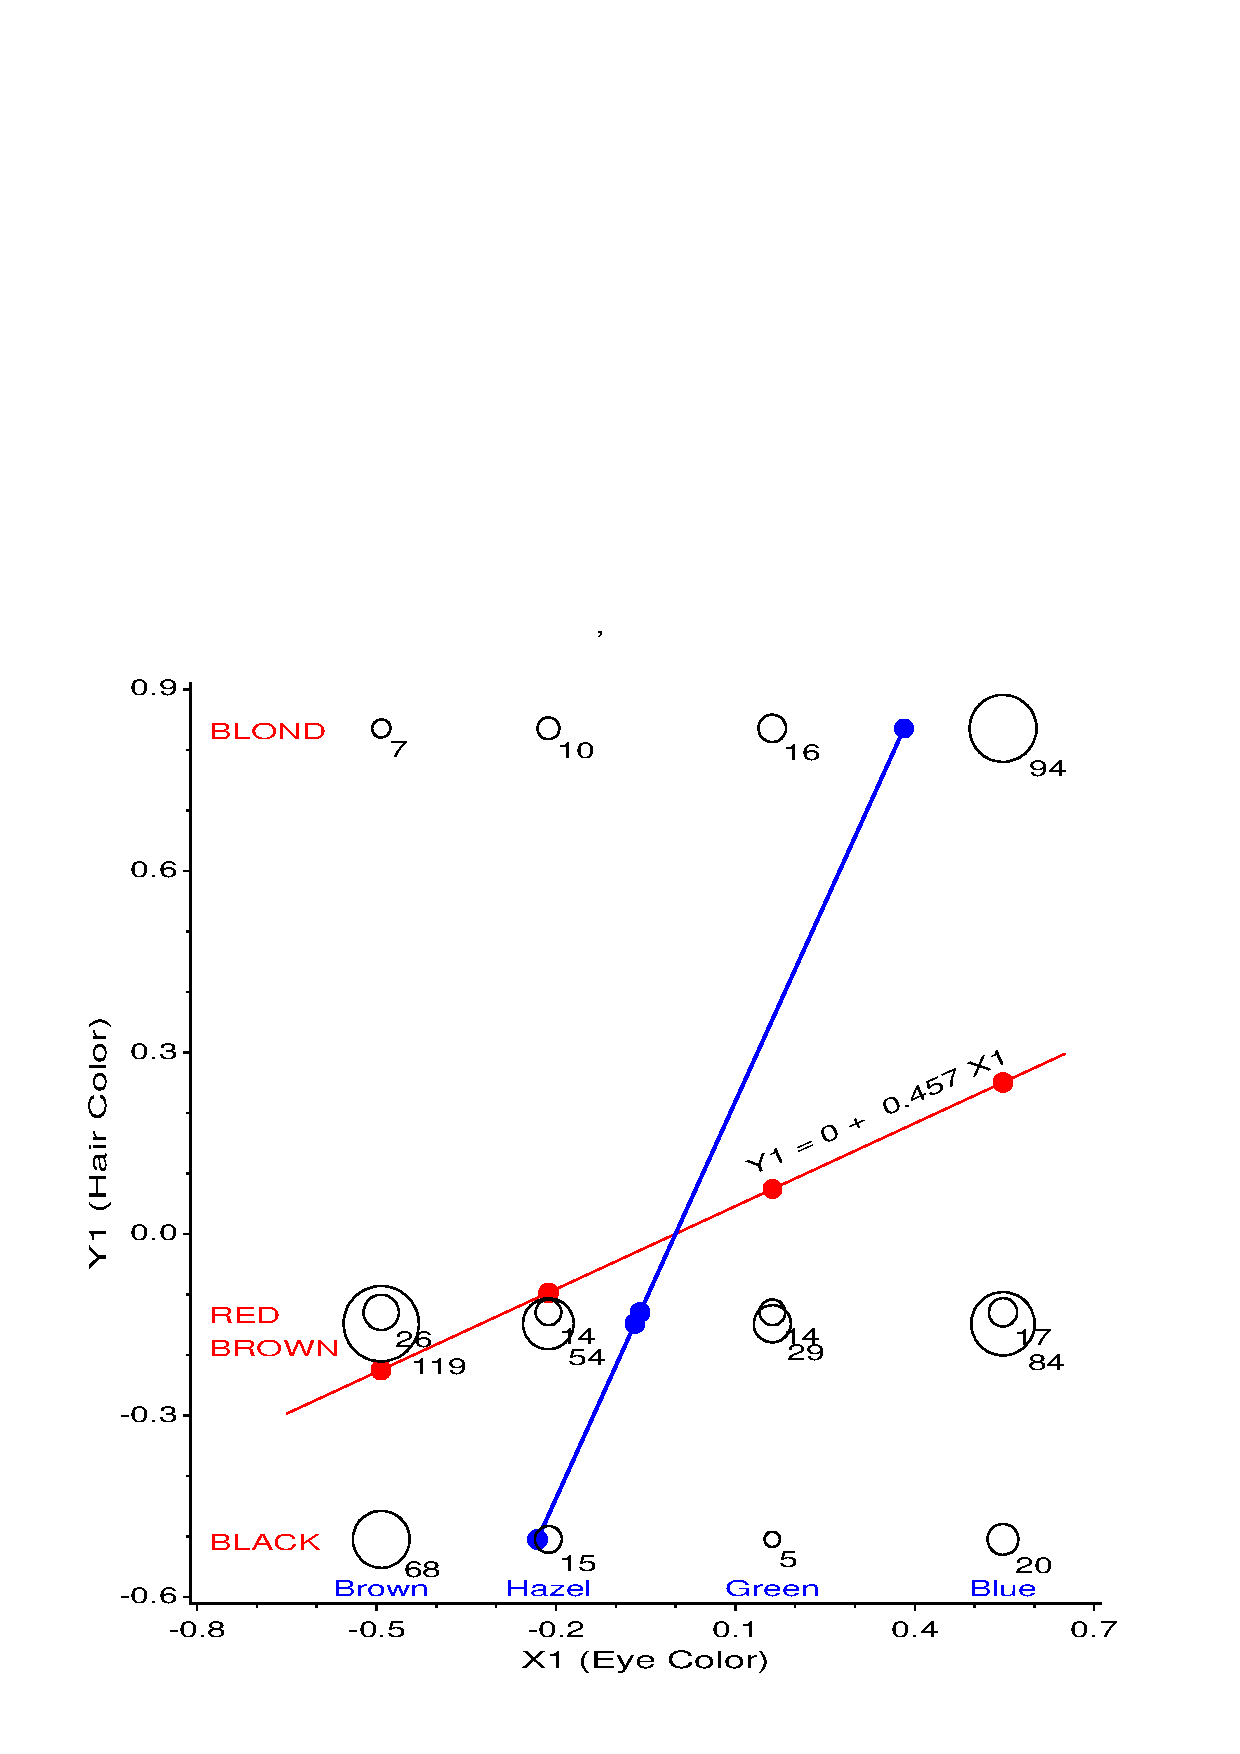
\includegraphics[scale=.6,clip]{ch5/fig/cascores}
  \caption[Simultaneous linear regressions of \CA\ scores for dimension 1]{Simultaneous linear regressions of \CA\ scores for dimension 1.  Using the optimal scores makes both regressions linear; choosing the scores associated with the largest singular value makes the two regressions most collinear.}\label{fig:cascores}
\end{figure}
%% input: /users/faculty/friendly/sasuser/catdata/cascores.sas
%% last modified: 04-Aug-98 13:31
\begin{listing}
*-- Annotate the row and column means;
proc means data=scores nway noprint;
   var y1;
   class x1;
   freq count;
   output out=ymeans mean=y1bar;
data ymeans;
   set ymeans;
   retain xsys  ysys '2' size 2;
   x = x1; y = y1bar;
   function = 'symbol'; text='dot'; color='red';  output;

proc means data=scores nway noprint;
   var x1;
   class y1;
   freq count;
   output out=xmeans mean=x1bar;
data xmeans;
   set xmeans;
   retain xsys  ysys '2' size 2 line 4;
   x = x1bar; y = y1;
   function = 'symbol'; text='dot'; color='blue';  output;
   if _n_=1 then function='move';
      else function='draw';
   output;

*-- Annotate the row and column labels;
data label1;
   set scores(keep=eye hair x1 y1);
   where eye='Brown';
   retain xsys ysys '2' color 'red    ' function 'label   ';
   if hair='BROWN' then position='9';
      else position='6';
   x = -.78; y = y1; text = hair;
data label2;
   set scores(keep=eye hair x1 y1);
   where hair='BLACK';
   retain xsys ysys '2' position '5' color 'blue' function 'label   ';
   x = x1; y = -.58; text = eye;

*-- Get slope and intercept of (weighted) regression line;
proc reg data=scores outest=parms noprint;
   model y1 = x1;
   weight count;

data line;
   set parms (keep=x1 intercep);
   drop x1 intercep;
   length text $20;
   
   *-- Draw (weighted) regression line;
   xsys='2'; ysys='2'; color='red   ';
   x=-0.65; y = intercep + x1 * x; function='MOVE    '; output;
   x= 0.65; y = intercep + x1 * x; function='DRAW    '; output;
   x= 0.35; y = intercep + x1 * x; function='LABEL   '; color='black';
   angle = atan(x1) * (45/atan(1)); position='2';
   text = 'Y1 = 0 + ' || put(x1,6.3) || ' X1';  output;
   
*-- Combine the annotate data sets;
data labels;
   length text $20;
   set label1 label2 line ymeans xmeans;

proc gplot data=scores;
   bubble y1 * x1 = count / 
      blabel bsize=8 bscale=area
      vaxis=axis1 haxis=axis2 hm=2 vm=2 anno=labels;
   axis1 order=(-.6 to .9 by .3) label=(h=1.8 a=90 'Y1 (Hair Color)');
   axis2 order=(-.8 to .7 by .3) label=(h=1.8      'X1 (Eye Color)');
   \end{listing}

Note that the slope of the line for $Y1\given X1$ in \figref{fig:cascores} is 0.457, the largest singular value and the largest canonical correlation.
If we were to repeat these steps using the \CA\ scores $X2$ and $Y2$
on dimension 2, we would find another pair of linear regressions, with
a slope of 0.149 for $Y2\given X2$, the second singular value.


\ixon{correspondence analysis!multi-way tables}
\section{Multi-way tables}\label{sec:ca-multiway}

A three- or higher-way table can be analyzed by correspondence
analysis in several ways.
\ixon{correspondence analysis!stacking}
Multiple correspondence analysis (MCA), described in \secref{sec:mca},
is an extension of simple
\CA\ which analyzes simultaneously all possible two-way tables
contained within a \mway\ table.
Another approach, described here, is called 
\glossterm{stacking}.
\ix{interactive coding}
A
three-way table, of size \(I \times  J \times  K\) can be sliced into
\(I\) two-way tables, each \(J \times  K\).  If the slices are
concatenated vertically, the result is one two-way table, of size \((
I \times  J ) \times  K\).  In effect, the first two variables are
treated as a single composite variable with \(IJ\) levels, which represents the main
effects and interaction between the original variables that were
combined.
\Citet{HeijdenLeeuw:85}
discuss this use of
correspondence analysis for multi-way tables and show how \emph{each} way of
slicing and stacking a contingency table corresponds to the analysis
of a specified \loglin\ model.
Like the mosaic display, this provides another way to visualize the relations
in a \loglin\ model.

In particular, for the three-way table that is reshaped as a table of
size \(( I \times  J ) \times  K\), the \CA\
solution analyzes residuals from the log-linear model [AB] [C].  That
is, for such a table, the \(I \times  J\) rows represent the joint
combinations of variables A and B.  The expected frequencies under
independence for this table are
\begin{equation}\label{eq:mij-k}
  m_{[ij]k} = \frac{ n_{[ij]+} \,  n_{[+]k} }{n}
 = \frac{ n_{ij+} \,  n_{++k} }{n}
\end{equation}
which are the ML estimates of expected frequencies for the log-linear
model [AB] [C].  The \(\chi^2\) that is decomposed by \CA\ is the Pearson
\(\chi^2\) for this log-linear model.  When the table is stacked as
\(I \times  ( J \times  K )\) or \(J \times  ( I \times  K )\),
correspondence analysis decomposes the residuals from the log-linear
models [A] [BC] and [B] [AC], respectively.
\Citet{HeijdenLeeuw:85}
show how a generalized form of correspondence analysis
can be interpreted as decomposing the difference between two specific
log-linear models, so their approach is more general than is illustrated
here.

This approach to the \CA\ of \mway\ tables is easily carried out with the
\proc{CORRESP} and the \macro{CORRESP}.  With the procedure, use the
\stmt{TABLES}{CORRESP} and list the variables to be combined interactively
as either the row or column variables (separated by a comma).
For example,  the \CA\ of residuals from the model [A B][C] of joint independence
\eqref{eq:mij-k} is specified by:

\begin{listing}
proc corresp cross=row;
   tables A B, C;
   weight count;
\end{listing}
The \opt{CROSS}{CORRESP} specifies that all combinations of the levels
of A and B are to define the rows of the \ctab.%
\footnote{If this option is omitted, the separate levels of each of
A and B define the table rows.}

For the \macro{CORRESP}, the
list the variables
in the \mparm{TABLES=}{CORRESP} separated by a \texttt{/},%
\footnote{You can also use a comma, but then the \mparm{TABLES=}{CORRESP}
must be quoted with the \pname{\%str()} macro function, e.g.,
\pname{TABLES=\%str(A B, C)}.}
and include \pname{CROSS=BOTH|ROW|COL} in the \mparm{OPTIONS=}{CORRESP}.
The following statement is equivalent to that above:
\begin{listing}
%corresp(options=cross=row,
   tables=A B/ C, weight=count);
\end{listing}

\begin{Example}[suicide1]{Suicide rates in Germany}

To illustrate the use of correspondence analysis for the analysis for
three-way tables, we use data on suicide rates in West Germany
(presented in \tabref{tab:suidat})
classified by age, sex, and method of suicide used.  The data, from
\citet[Table 1]{Heuer:79}
have been discussed by
\citet{Friendly:91,Friendly:94a,HeijdenLeeuw:85}
and others.
The original \(2
\times  17 \times  9\) table contains 17 age groups from 10 to 90 in
5-year steps and 9 categories of suicide method, listed in \datref{dat:suicide}. 
To avoid extremely
small cell counts and cluttered displays,
this example uses a reduced table in which age
groups are combined in 15 year intervals except for the last
interval, which includes age 70 - 90; the methods ``toxic gas'' and
``cooking gas'' were collapsed and methods ``knife'' and ``other''
were deleted, giving the \(2 \times  5 \times  6\) table shown in
\tabref{tab:suidat}.  These changes do not affect the general
nature of the data or conclusions drawn from them.

\begin{table}[htb]
 \caption[Suicide Data]{Suicide Data. Frequencies of Suicide by Age, Sex, and
Method. (Heuer, 1979)}
 \label{tab:suidat}
\begin{center}
 \begin{tabular}{|rr rrrrrr|}
 \hline
      &     & \multicolumn{6}{c|}{\bfseries\large Method} \\
		        \cline{3-8}
  {\bfseries\large Sex} & {\bfseries\large Age} & Poison & Gas & Hang & Drown & Gun & Jump \\ 
   \hline 
  M & 10-20 & 1160 & 335 & 1524 &  67 & 512 & 189 \\ 
  M & 25-35 & 2823 & 883 & 2751 & 213 & 852 & 366 \\ 
  M & 40-50 & 2465 & 625 & 3936 & 247 & 875 & 244 \\ 
  M & 55-65 & 1531 & 201 & 3581 & 207 & 477 & 273 \\ 
  M & 70-90 &  938 & 45  & 2948 & 212 & 229 & 268 \\ [2mm]
%   \hline 
  F & 10-20 &  921 &  40 & 212  &  30 & 25 & 131 \\ 
  F & 25-35 & 1672 & 113 & 575  & 139 & 64 & 276 \\ 
  F & 40-50 & 2224 &  91 & 1481 & 354 & 52 & 327 \\ 
  F & 55-65 & 2283 &  45 & 2014 & 679 & 29 & 388 \\ 
  F & 70-90 & 1548 &  29 & 1355 & 501 &  3 & 383 \\ 
 \hline
 \end{tabular}
\end{center}
\end{table}

\tabref{tab:suifit} shows the results of all possible hierarchical
log-linear models for the suicide data.  It is apparent that none of
these models has an acceptable fit to the data.  Given the enormous
sample size (\(n = 48,177\)), even relatively small departures from
expected frequencies under any model would appear significant,
however.
\begin{table}[htb]
 \caption{Goodness-of-fit for hierarchical
log-linear models for the suicide data}\label{tab:suifit}
 \begin{center}
 \begin{tabular}{lrrrrr}
 \hline
  Model & df & L.R. \(G^2\) & G.F. \(\chi^2\) \\ 
   \hline
  $[M] [A] [S]$ & 49 & 10119.60 & 9908.24 \\ [2mm]
%
  $[M] [AS]$ & 45 & 8632.0 & 8371.3 \\ 
  $[A] [MS]$ & 44 & 4719.0 & 4387.7 \\ 
  $[S] [MA]$ & 29 & 7029.2 & 6485.5 \\ [2mm]
%
  $[MS] [AS]$ & 40 & 3231.5 & 3030.5 \\ 
  $[MA] [AS]$ & 25 & 5541.6 & 5135.0 \\ 
  $[MA] [MS]$ & 24 & 1628.6 & 1592.4 \\ [2mm]
%
  $[MA] [MS] [AS]$ & 20 & 242.0 & 237.0 \\ 
 \hline
 \end{tabular}
 \end{center}
\end{table}


The decision about which variables to combine interactively relates
more to the choice of which associations are to be displayed,
and which are to be ignored, rather than to the choice of a best-fitting
model.  For example,
\CA\ applied to the [AS] by [M] table helps to
show the nature of the association between method of suicide and the
joint age-sex combinations and decomposes the \(\chi^2 = 8371\) for
the log-linear model [AS] [M].  This analysis would ignore the
age-sex association, however.

To carry out this analysis with the
data in the form of a frequency \Dset\
(with variables \texttt{age}, \texttt{sex}, \texttt{method}, and
\texttt{count}),
call the \proc{CORRESP} with the statements
\begin{listing}
proc corresp data=suicide cross=row short;
   table age sex, method;
   weight count;
run;
\end{listing}
Or, to perform this analysis and produce the graphical display in
\figref{fig:suicide51}, call the \macro{CORRESP} as
\begin{listing}
axis1 order=(-.7 to .7 by .7) length=6.5 in label=(a=90 r=0);
axis2 order=(-.7 to .7 by .7) length=6.5 in;
%corresp(data=suicide, tables=%str(age sex, method), weight=count,
        options=cross=row short, vaxis=axis1, haxis=axis2);
\end{listing}

\begin{figure}[htb]
  \centering
  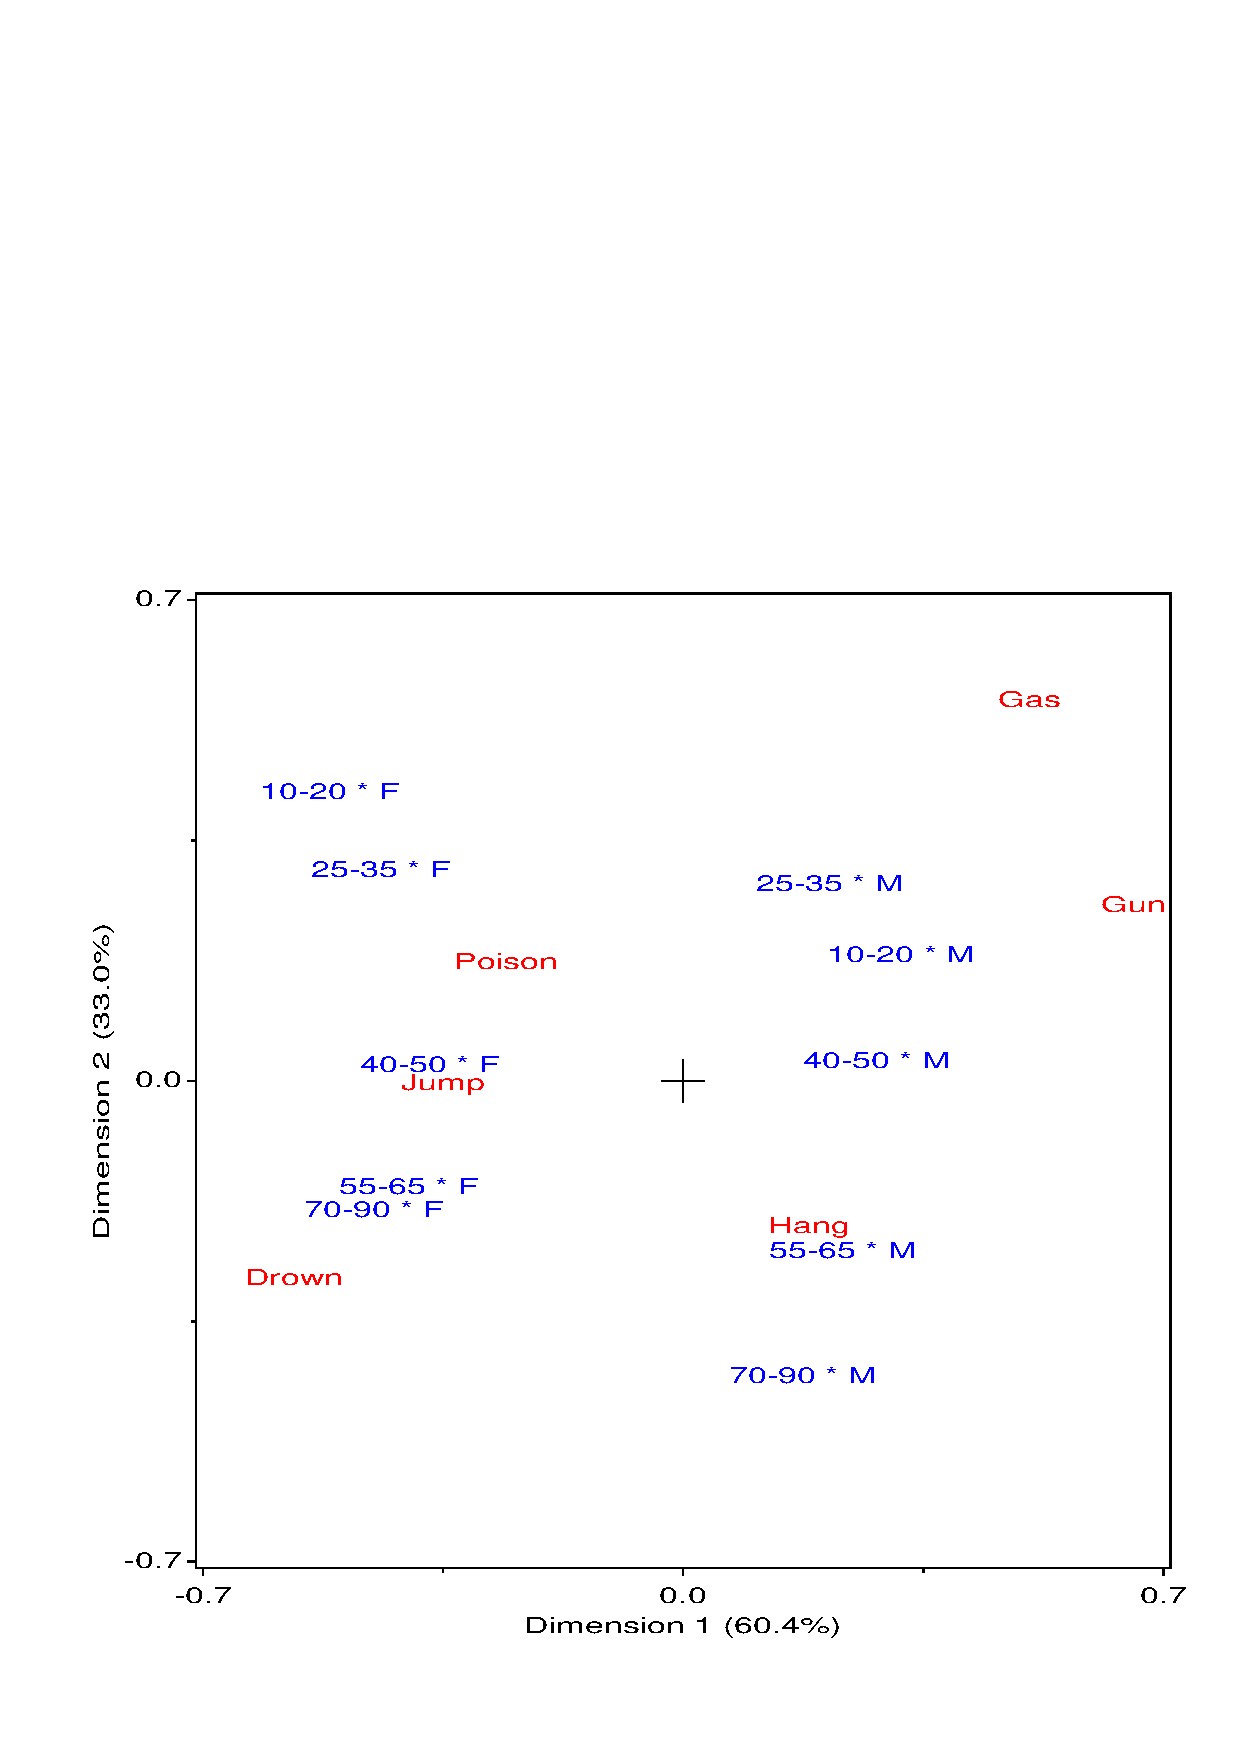
\includegraphics[scale=.7,clip=true]{ch\thechapter/fig/suicide51}
  \caption{Two-dimensional correspondence analysis
solution for the [AS] [M] multiple table}\label{fig:suicide51}
\end{figure}

The printed results, shown partially in \outref{out:suicide5} indicate that over 93\% of the association between the age-sex categories and method of
suicide can be represented well in two dimensions.

\begin{Output}[htb]
\caption{Chi-Square Decomposition for suicide data}\label{out:suicide5}
\begin{output}
                   Inertia and Chi-Square Decomposition

     Singular  Principal Chi-
     Values    Inertias  Squares Percents   12   24   36   48   60
                                         ----+----+----+----+----+---
     0.32138   0.10328   5056.91  60.41% *************************
     0.23736   0.05634   2758.41  32.95% **************
     0.09378   0.00879    430.55   5.14% **
     0.04171   0.00174     85.17   1.02%
     0.02867   0.00082     40.24   0.48%
               -------   -------
               0.17098   8371.28 (Degrees of Freedom = 45)
\end{output}
\end{Output}
\ixd{suicide}

The plot of the \CA\ scores for the rows (sex-age combinations) and
columns (methods) in \figref{fig:suicide51}
shows residuals from the log-linear model [AS] [M].
Thus, it shows the two-way associations of sex \(\times\) method, age
\(\times\) method, and the three-way association, sex \(\times\) age
\(\times\) method which are set to zero in the model [AS] [M].  The
possible association between sex and age is not shown in this plot.

Dimension 1 in the plot separates males and females.  This dimension
indicates a strong difference between suicide profiles of males and
females.  The second dimension is mostly ordered by age with younger
groups at the top and older groups at the bottom.  Note also that the
positions of the age groups are approximately parallel for the two
sexes.  Such a pattern indicates that sex and age do not interact in
this analysis.  The relation between the age - sex groups and methods
of suicide can be interpreted in terms of similar distance and
direction from the origin, which represents the marginal row and
column profiles.  Young males are more likely to commit suicide by
gas or a gun, older males by hanging, while young females are more
likely to ingest some toxic agent and older females by jumping or
drowning.

For comparison, the mosaic display for the [AS] [M] table
is shown in \figref{fig:mosaic6b}.
The methods have been arranged in order
of the method scores on the first dimension of the CA solution
of \figref{fig:suicide51}.
This figure
again shows the prevalence of GUN and
GAS, among younger males and decreasing with age, whereas use of HANG
increases with age.  For females, these three methods are used less
frequently than would be the case if method were independent of age
and sex, whereas POISON, JUMP, and DROWN occur more often.

\begin{figure}[!htb]
  \centering
  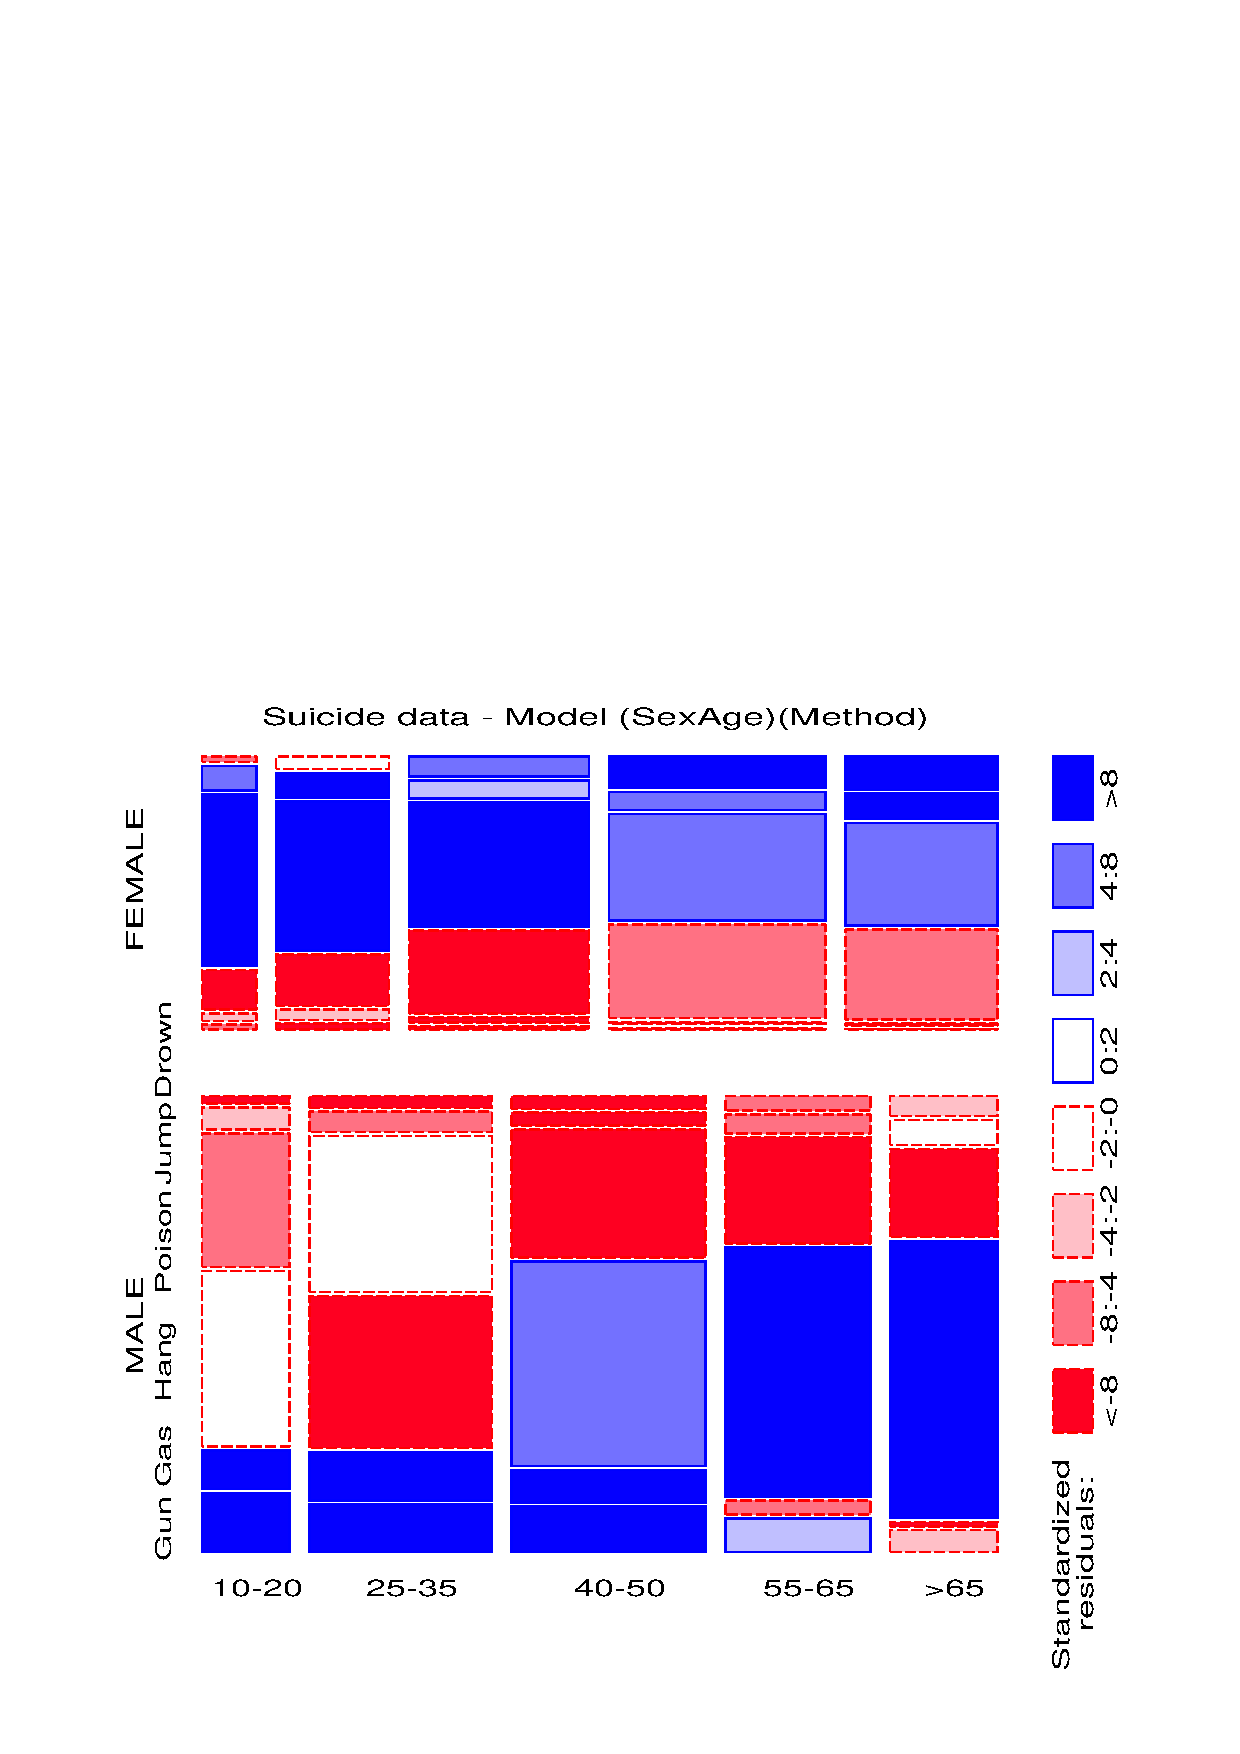
\includegraphics[scale=.6,clip]{ch\thechapter/fig/mosaic6b}
  \caption[Mosaic display showing deviations from
model AS, M]{Mosaic display showing deviations from
model [AS] [M].  The methods have been reordered according to their
positions on Dimension 1 of the correspondence analysis solution for
the [AS] [M] table.}\label{fig:mosaic6b}
\end{figure}
\end{Example}
\ixoff{correspondence analysis!stacking}

\subsection{Marginal tables and supplementary variables}
\ix{correspondence analysis!supplementary variables}
An \nway\ table in frequency form or case form is automatically collapsed
over factors which are not listed in the
\stmt{TABLES}{CORRESP} (or in the macro \mparm{TABLES=}{CORRESP}).
The analysis gives a marginal model for the categorical variables which
\emph{are} listed.  

The positions of the categories of the omitted variables
may nevertheless be recovered, by treating them as supplementary variables.
A supplementary variable is ignored in finding the CA solution,
but its categories are then projected into that space.

To illustrate, the statement below lists only the \texttt{age}
and \texttt{method} variables, and hence produces an analysis
collapsed over \texttt{sex}.
This ignores not only the effect of sex itself,
but also all associations of age and method with sex,
which (from \tabref{tab:suifit}) are substantial.
\begin{listing}
%corresp(data=suicide, tables=%str(age, method),  weight=count);
\end{listing}

This analysis and 
the graph produced do not include category points for \texttt{sex},
but we may re-do the same analysis including \texttt{sex} as a supplementary
variable as shown below.

\begin{listing}
%corresp(data=suicide, tables=%str(age sex, method), sup=sex,
   weight=count, inc=0.2 0.1, dimlab=Dim);
\end{listing}
Note that \texttt{sex} must also be listed among the \pname{TABLES}
variables.
\begin{figure}[htb]
  \centering
  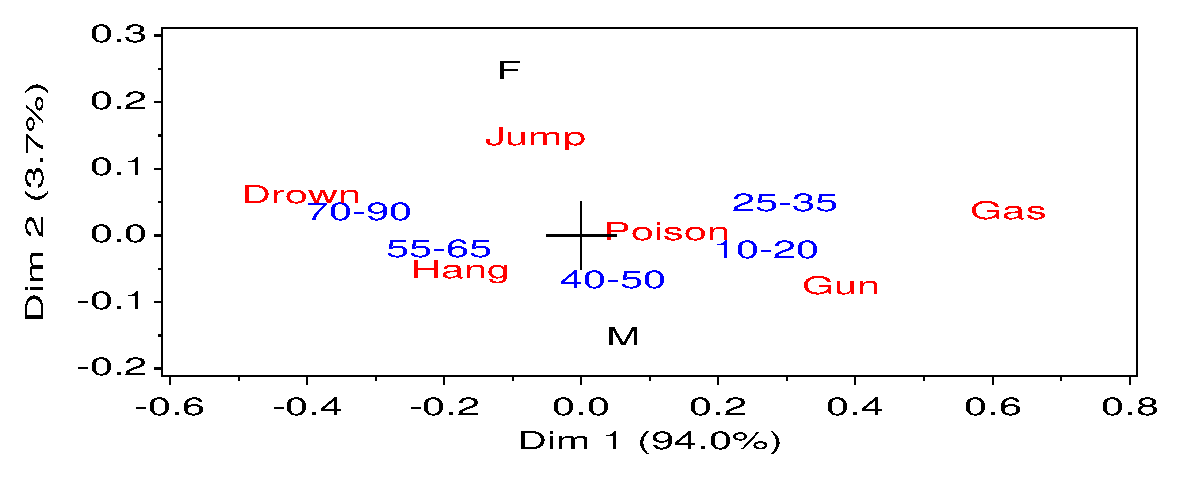
\includegraphics[scale=.7,clip=true]{ch\thechapter/fig/suicide6}
  \caption[Two-dimensional correspondence analysis
solution for the A M marginal table]{Two-dimensional correspondence analysis
solution for the [A] [M] marginal table.
Category points for Sex are shown as supplementary points.}\label{fig:suicide6}
\end{figure}

This analysis produces a $\chisq (20) = 2917.83$,
the same as the Pearson chi-square for the [A] [M] marginal table.
The plot (\figref{fig:suicide6}) is essentially one-dimensional,
where Dimension 1 reflects age most prominently.
Comparing this graph with \figref{fig:suicide51},
you may see that ignoring sex has collapsed the differences between
males and females which were the dominant feature of the analysis
including sex.
However, as in \figref{fig:suicide51}, the supplementary points for sex 
show a greater tendency for females to use JUMP, and for males to use
HANG or GUN.

\ixon{correspondence analysis!multiple}
\section{Multiple correspondence analysis}\label{sec:mca}

Multiple \CA\ (MCA) is designed to display the relationships of the categories
of two or more discrete variables.  Again, there are several complementary
ways of defining MCA as an optimal scaling of categorical data.
The most typical starts by defining indicator (``dummy'') variables
for each category and reexpresses the \nway\ \ctab\ in the form
of a cases by variables indicator matrix, $\mat{Z}$.
Simple \CA\ for a two-way table can, in fact, be derived as the
canonical correlation analysis of the indicator matrix.
Unfortunately, the generalization to more than two variables follows
a somewhat different path, so that simple CA does not turn out to be
precisely a special case of MCA in some respects, particularly in the
decomposition of an interpretable \chisq\ over the dimensions in
the visual representation.

Nevertheless, MCA does provide a useful graphic portrayal of the
\emph{bivariate} relations among any number of categorical variables,
and has close relations to the mosaic matrix (\secref{sec:mosmat}).
And, if its limitations are understood, it may be helpful in
understanding large, multivariate categorical \Dsets.

\subsection{Bivariate MCA}\label{sec:mca-bi}
\ixon{multiple correspondence analysis!bivariate}
For the hair color, eye color data, the indicator matrix $\mat{Z}$
has 592 rows and $4+4=8$ columns.  The columns refer to the eight
categories of hair color and eye color and the rows to the students
in Snee's \citeyear{Snee:74} sample.
The indicator matrix is shown in \tabref{tab:haireye2}, where
to save space each combination of hair color and eye color actually
corresponds to the number of repeated rows represented by the $n_{ij}$
column.
Variable $h_1$ represents the hair category Black, and
Variable $e_1$ represents the eye category Brown,
so the first row of table \tabref{tab:haireye2}
corresponds to the 68 people with black hair and brown eyes.
The indicator matrix $\mat{Z}$ thus has 68 identical rows with that response
pattern.
\begin{table}[htb]
 \caption{Indicator matrix for hair color, eye color data (grouped)}\label{tab:haireye2}
 \begin{center}
 \begin{tabular}{|ll r | rrrr|rrrr|}
 \hline
       &     &     & \multicolumn{4}{c|}{Hair} & \multicolumn{4}{c|}{Eye} \\
  Hair & Eye & $n_{ij}$ 
  & $h_1$ & $h_2$ & $h_3$ & $h_4$ 
  & $e_1$ & $e_2$ & $e_3$ & $e_4$ 
  \\ 
 \hline
  BLACK & Brown &  68 & 1 & 0 & 0 & 0 & 1 & 0 & 0 & 0 \\ 
  BROWN & Brown & 119 & 0 & 1 & 0 & 0 & 1 & 0 & 0 & 0 \\ 
  RED   & Brown &  26 & 0 & 0 & 1 & 0 & 1 & 0 & 0 & 0 \\ 
  BLOND & Brown &   7 & 0 & 0 & 0 & 1 & 1 & 0 & 0 & 0 \\  [1mm]
  BLACK & Hazel &  15 & 1 & 0 & 0 & 0 & 0 & 1 & 0 & 0 \\ 
  BROWN & Hazel &  54 & 0 & 1 & 0 & 0 & 0 & 1 & 0 & 0 \\ 
  RED   & Hazel &  14 & 0 & 0 & 1 & 0 & 0 & 1 & 0 & 0 \\ 
  BLOND & Hazel &  10 & 0 & 0 & 0 & 1 & 0 & 1 & 0 & 0 \\  [1mm]
  BLACK & Green &   5 & 1 & 0 & 0 & 0 & 0 & 0 & 1 & 0 \\ 
  BROWN & Green &  29 & 0 & 1 & 0 & 0 & 0 & 0 & 1 & 0 \\ 
  RED   & Green &  14 & 0 & 0 & 1 & 0 & 0 & 0 & 1 & 0 \\ 
  BLOND & Green &  16 & 0 & 0 & 0 & 1 & 0 & 0 & 1 & 0 \\  [1mm]
  BLACK & Blue  &  20 & 1 & 0 & 0 & 0 & 0 & 0 & 0 & 1 \\ 
  BROWN & Blue  &  84 & 0 & 1 & 0 & 0 & 0 & 0 & 0 & 1 \\ 
  RED   & Blue  &  17 & 0 & 0 & 1 & 0 & 0 & 0 & 0 & 1 \\ 
  BLOND & Blue  &  94 & 0 & 0 & 0 & 1 & 0 & 0 & 0 & 1 \\ 
 \hline
 (Totals) &       & 592 
 & 220 & 215 & 93 & 64 
 & 108 & 286 & 71 & 127 
 \\ 
 \hline
 \end{tabular}
 \end{center}
\end{table}




Each row of the indicator matrix sums to 2, the number of variables
represented, and each category column sums to the marginal total for
that category.
Note that appropriate subsets of the rows are in a sense synonymous with
the column categories.  For example, the first four rows of the table
are all those with brown eyes, so these rows represent $e_1$.

If the indicator matrix is partitioned as
$\mat{Z} = [ \mat{Z}_1 , \mat{Z}_2 ]$, corresponding to the two sets of
categories, then the contingency table is given by
$\mat{N} = \mat{Z}_1 \trans \mat{Z}_2$.
Then, MCA can be described as the application of the simple \CA\
algorithm to the indicator matrix $\mat{Z}$.
This analysis would yield scores for the rows of $\mat{Z}$ (the cases)
and for the columns (the categories).
As in simple CA, each row point is the weighted average of the scores
for the column categories, and each column point is the weighted average
of the scores for the row observations.

Consequently, the point for any category is the centroid of all the
observations with a response in that category, and
all observations with the same response pattern coincide.
As well, the origin reflects the weighted average of the categories for
\emph{each} variable.  As a result, category points with low marginal
frequencies will be located further away from the origin,
while categories with high marginal frequencies will be closer to the
origin.
For a binary variable, the two category points will appear on a line
through the origin, with distances inversely proportional to their
marginal frequencies.

\begin{Example}[haireye4]{Hair color and eye color}
For expository purposes,
we illustrate the analysis of the indicator matrix below for the hair color,
eye color data.
MCA is usually carried out more simply through analysis of
the ``Burt matrix'', described in the following subsection.

The indicator matrix may be constructed from the \Dset\ in \ctab\ form
as shown below, using \PROC{TRANSPOSE} and a \Dstp\ to calculate
the dummy variables from the original row and column variables.%
\footnote{These steps actually create a design matrix, with one
observation per category, with the frequencies, $n_{ij}$, as shown in
\tabref{tab:haireye2}.  In the \pname{\%corresp} step, the
\pname{count} variable is used as a weight, to reproduce the
indicator matrix.}
%% input: /Users/friendly/sasuser/catdata/mcahair.sas
%% last modified: 24-Jul-99 11:19
\begin{listing}
data haireye;
   input  EYE $ BLACK BROWN RED BLOND ;
datalines;
         Brown    68   119    26     7    
         Hazel    15    54    14    10    
         Green     5    29    14    16    
         Blue     20    84    17    94    
;
*-- Reshape data to frequency form;
proc transpose data=haireye out=haireye2;
   var BLACK BROWN RED BLOND;
   by eye notsorted;

*-- Create dummy variables;
data haireye2;
   set haireye2 (rename= (_name_=hair col1=count));
   h1 = (hair='BLACK');   h2 = (hair='BROWN');
   h3 = (hair='RED');     h4 = (hair='BLOND');
   e1 = (eye ='Brown');   e2 = (eye ='Hazel');
   e3 = (eye ='Green');   e4 = (eye ='Blue');
\end{listing}


Analysis of the indicator matrix (the \Dset\ \pname{haireye2})
is conveniently carried out with the \macro{CORRESP}.
\begin{listing}
axis1 length=6.5 IN order=(-1.2 to 2 by 0.4) label=(a=90);
axis2 length=6.5 IN order=(-1.2 to 2 by 0.4);

%corresp(data=haireye2, id=id, var=h1-h4 e1-e4, weight=count,
   symbols=none dot, pos=5 -, vaxis=axis1, haxis=axis2, anno=labels, gplot=no);
\end{listing}

Some additional Annotation steps (not shown) to add some lines to
the \ADS\ \pname{labels} produces \figref{fig:mcahair},
in which the row and column points are shown in principal coordinates.
Comparing this with \figref{fig:corresp3}, we see that the pattern of
the hair color and eye color categories is the same in the analysis of
the contingency table (\figref{fig:corresp3}) and the analysis of the
indicator matrix (\figref{fig:mcahair}), except that the axes are scaled
differently---the display has been stretched along the second (vertical)
dimension.
Indeed, it may be shown \citep{Greenacre:84}
that the two displays are identical, except for changes in scales along
the axes.
There is no difference at all between the displays in standard coordinates.
\citet[pp. 130--134]{Greenacre:84} describes the precise relations
between the geometries of the two analyses.

%% one figure
\begin{figure}[htb]
  \centering
  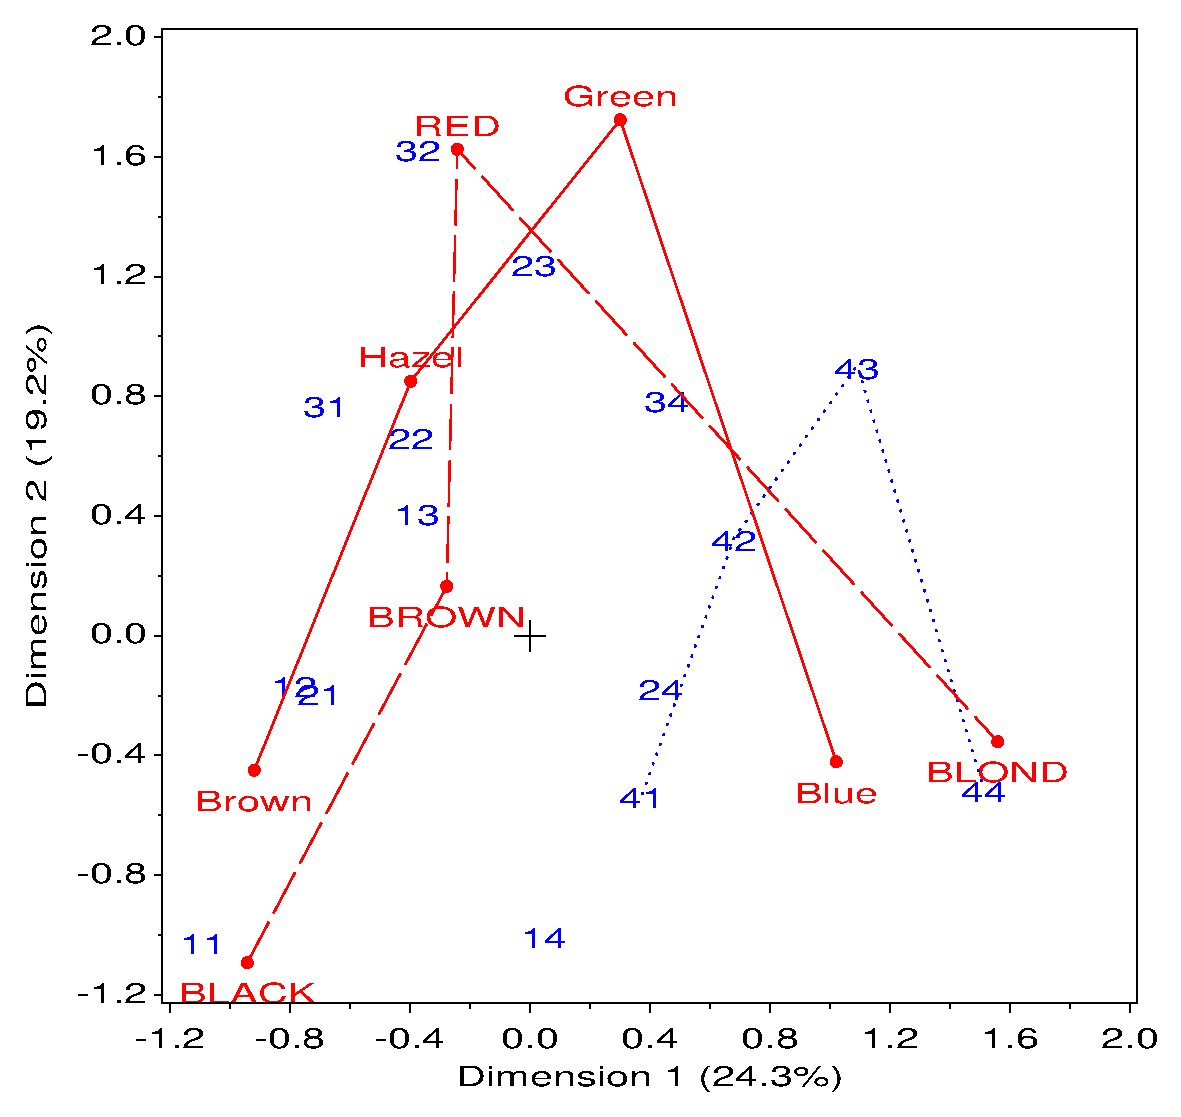
\includegraphics[scale=.7,clip]{ch5/fig/mcahair}
  \caption[Correspondence
  analysis of the indicator matrix Z for the hair color, eye color data]{Correspondence
  analysis of the indicator matrix $\mat{Z}$ for the hair color, eye color data.
  The category points are joined for the hair color and eye color categories.
  Observation (row) points, are labeled by the subscripts of $h, e$.
  The dotted line connects those with blond hair.}%
  \label{fig:mcahair}
\end{figure}

\figref{fig:mcahair} also plots the row points (corresponding to the observations) from this analysis.  Each point is labeled by the subscripts,
$ij$, of $h_i e_j$, and actually represents $n_{ij}$ rows
from the indicator matrix
plotted at the point.  For example, the points labeled `41'--`44'
represent all the observations with blond hair.
There are actually 94 observations at the point `44', representing the
blue-eyed blonds.
\end{Example}


A major difference between analysis of the \ctab\ and analysis of the
indicator matrix is in the decomposition of inertia and $\chisq$
for the dimensions.
The inertias for the analysis of the indicator matrix are shown in
\outref{out:mcahair.1}.
Comparing these values with \outref{out:corresp3.1},
we see that 6 dimensions are shown in the analysis of the indicator matrix,
while only 3 are shown in the analysis of the \ctab.
The inertias and $\chisq$ values differ less dramatically than
in \outref{out:corresp3.1}, and the inertias sum to exactly 3.0 in the
indicator matrix analysis.

For a two-way table of size ($J_1 \times J_2$), CA of the indicator matrix
produces $J_1 + J_2 - 2$ dimensions, but it turns out that half of these
are artifacts which should be disregarded, and these correspond to those
with principal inertias $\lambda^2 < \frac{1}{2}$.
The total inertia depends not on the $\chisq$ for association
as in simple CA of the \ctab,
but is simply $(J_1 + J_2 - 2) / 2$.
The singular values of the non-trivial dimensions in the
analysis of $\mat{Z}$ (symbolized as $\lambda_i^Z$)
are related to those ($\lambda_i$) of the analysis of the \ctab\ by
\begin{equation*}%\label{eq:lzn}
 \lambda_i^Z = \{ \frac{1}{2} [ 1 + \lambda_i ] \}^{1/2}
 \period
\end{equation*}
We can recover the singular values from the analysis of the \ctab\
by inverting this relation, which gives
\begin{equation}\label{eq:lnz}
 \lambda_i = 2  (\lambda_i^Z)^2 - 1
 \period
\end{equation}
For example, using the first singular value, $\lambda_1^Z = 0.8535$ from
\outref{out:mcahair.1} in \eqref{eq:lnz}
gives $\lambda_1 = 2 ({0.8535} ^ 2) - 1 =  0.4569$,
the value in \outref{out:corresp3.1}.

\begin{Output}[htb]
\caption{Correspondence analysis output for the indicator matrix of the hair color, eye color data}\label{out:mcahair.1}
\small
\verbatiminput{ch5/out/mcahair.1}
\end{Output}

%\begin{Output}[htb]
%\caption{Correspondence analysis output, row and column scores, for the hair color, eye color data}\label{out:mcahair.2}
%\small
%\verbatiminput{ch5/out/mcahair.2}
%\end{Output}

\subsection{The Burt matrix}\label{sec:mca-burt}
\ixon{Burt matrix}
The same solution for the category points as in the
analysis of the indicator matrix may be obtained more simply
from the so-called ``Burt matrix'' \citep{Burt:50},
\begin{equation*}%\label{eq:burt2}
 \mat{B} = \mat{Z}\trans \mat{Z}
 =
 \left[
 \begin{array}{ll}
 \mat{N}_{1} & \mat{N} \\
 \mat{N}\trans & \mat{N}_{2} \\
 \end{array}
 \right]
 \comma
\end{equation*}
where $\mat{N}_{1}$ and $\mat{N}_{2}$ are diagonal matrices containing
the marginal frequencies of the two variables (the column sums of
$\mat{Z}_1$ and $\mat{Z}_2$).

The standard coordinates from an analysis of the Burt matrix
$\mat{B}$ are identical to those of $\mat{Z}$.
The singular values of $\mat{B}$ are the squares of those of $\mat{Z}$;
however, the \proc{CORRESP} compensates by taking the square root,
so the same values are printed.

The \proc{CORRESP} and the \macro{CORRESP} calculate the
Burt matrix when the \opt{MCA}{CORRESP} is used, and the category
variables are given in the \stmt{TABLES}{CORRESP}.
For the hair color, eye color data, we obtain the same category points
and inertias as the analysis in \exref{ex:haireye4} with the following
statement, using the table variables \pname{hair} and \pname{eye},
rather than the indicator variables \pname{H1-H4 E1-E4}.
\begin{listing}
%corresp(data=haireye2, tables=hair eye, weight=count, options=short mca,
   inc=0.4, xextra=0 1, pos=-, symbols=dot, colors=red);
\end{listing}
The Burt matrix is symmetric and the rows and columns both refer to
the hair, eye categories.
Only the column (category) points appear in the output and the plot.
\ixoff{multiple correspondence analysis!bivariate}

\subsection{Multivariate MCA}\label{sec:mca-multi}
The coding of categorical variables in an indicator matrix provides
a direct and natural way to extend this analysis to more than two variables.
If there are $Q$ categorical variables, and variable $q$ has $J_q$
categories, then the $Q$-way \ctab, of size
$J = \prod_{q=1}^Q J_q = J_1 \times J_2 \times \cdots \times J_Q$,
with a total of $n = n_{++\cdots}$ observations
may be represented by the partitioned $(n \times J)$ indicator matrix
$[ \mat{Z}_1 \, \mat{Z}_2  \, \dots \, \mat{Z}_Q ]$.

Then the Burt matrix is the symmetric partitioned matrix
\begin{equation*}
 \mat{B} = \mat{Z}\trans \mat{Z}
 =
 \left[
 \begin{array}{llll}
 \mat{N}_{[1]} & \mat{N}_{[12]} & \cdots & \mat{N}_{[1Q]}\\
 \mat{N}_{[21]} & \mat{N}_{[2]} & \cdots & \mat{N}_{[2Q]}\\
 \vdots        & \vdots         & \ddots  & \vdots       \\
 \mat{N}_{[Q1]} & \mat{N}_{[Q2]} & \cdots & \mat{N}_{[Q]}\\
 \end{array}
 \right]
 \comma
\end{equation*}
where again the diagonal blocks $\mat{N}_{[i]}$ contain the one-way
marginal frequencies.

Classical MCA (see, e.g., \cite{Greenacre:84,GowerHand:96})
can then be defined as a singular value decomposition of the matrix $\mat{B}$ which produces scores for the
categories of all variables so that the greatest proportion of the
bivariate, pairwise associations in all off-diagonal blocks is accounted for in
a small number of dimensions.
In this respect, MCA resembles multivariate methods for quantitative
data based on the joint bivariate correlation or covariance matrix
($\mat{\Sigma}$)
and there is some justification to regard the Burt matrix as the
categorical analog of $\mat{\Sigma}$.%
\footnote{For multivariate normal data, however, the mean vector and
covariance matrix are sufficient statistics, so all higher-way relations
are captured in the covariance matrix.  This is not true of the Burt
matrix.}

There is a close connection between this analysis and the bivariate mosaic
matrix (\secref{sec:mosmat}):
The mosaic matrix displays the residuals from independence for each
pair of variables, and thus provides a visual representation of the Burt matrix.
(The representation would be complete if the one-way margins
were drawn in the diagonal cells.)
The total amount of shading in all the individual mosaics
portrays the total pairwise associations decomposed by MCA.
See \citet{Friendly:99b} for further details.

In \secref{sec:mca-bi} we saw that, with $Q=2$ categorical variables,
analysis of the indicator matrix or the Burt matrix
produces twice as many dimensions as the analysis of the
equivalent \ctab; but only those whose principal inertias,
$(\lambda^Z)^2$, exceed $\frac{1}{2}$
are interesting, the remaining ones being artifacts.
When there are $Q>2$ variables represented in the Burt matrix,
it may be argued \citep{Greenacre:84,Greenacre:90} that the
interesting dimensions correspond to those with principal
inertia $> 1/Q$.

A more serious problem lies in the calculation of total inertia,
and therefore in the chi-square values and corresponding percentages
of association accounted for in some number of dimensions.
In simple CA, the total inertia is $\chisq /n$, and it therefore
makes sense to talk of percentage of association accounted for
by each dimension.
But in MCA of
the Burt matrix (with the square-root fixup provided by the \proc{CORRESP}),
the total inertia is simply $(J - Q)/Q = J/Q - 1$,
because that is what the analysis of the equivalent indicator matrix
would give.
The consequence is that the $\chisq$ percentages reported by
\PROC{CORRESP} are somewhat misleading, and give a rather pessimistic
view of the association accounted for in the two (or three) dimensions
usually plotted.
\ixoff{Burt matrix}

To more adequately reflect the percentage of association in MCA,
\citet{Benzecri:77} suggested the calculation of
\begin{equation*}%\label{eq:benzecri}
(\lambda_i^{\star})^2 =
{\left[ \frac{Q}{Q-1} ( \lambda_i^Z - (1/Q) ) \right]}^2
\end{equation*}
as the principal inertia due to the dimensions with $(\lambda^Z)^2 > 1/2$.
Benz{\'e}cri then expresses the contribution of each dimension as
$ (\lambda_i^{\star})^2 / \sum (\lambda_i^{\star})^2$,
with the summation over only dimensions with $(\lambda^Z)^2 > 1/2$.

Although this \emph{is} an improvement, it is somewhat \emph{ad hoc},
and not totally satisfactory.
\citet{Greenacre:88} develops an alternative analysis
called joint correspondence analysis (JCA)
which fits only the $Q \times (Q-1) /2$ off-diagonal blocks
of the Burt matrix.
\ix{correspondence analysis!joint}
\citet{Greenacre:90} then proposed to define the total inertia
as the average inertia in these off-diagonal blocks.%
\footnote{In \sasver{8}, the \proc{CORRESP} provides the
\pname{BENZECRI} and \pname{GREENACRE} options, which give more
reasonable and useful inertia contributions.
\ix{CORRESP@\texttt{CORRESP} procedure!GREENACRE@\texttt{GREENACRE} option}
\ix{CORRESP@\texttt{CORRESP} procedure!BENZECRI@\texttt{BENZECRI} option}
One of these options should be used for MCA in the \mparm{OPTIONS}{CORRESP}
with the \macro{CORRESP}.
}

For the interpretation of MCA plots, we note the following relations
\citep[\S 5.2]{Greenacre:84}:
\begin{itemize*}
\item The centroid of the categories for each discrete variable
is at the origin of the display.
\item The inertia contributed by a given variable increases with the
number of response categories.
\item For a particular variable,
the inertia contributed by a given category increases as the marginal
frequency in that category \emph{decreases}.
\item The category points for a binary variable lie on a line
through the origin.  The distance of each point to the origin is
inversely related to the marginal frequency.
\end{itemize*}

\begin{Example}[titanic2]{Survival on the \emph{Titanic}}
An MCA analysis of the \emph{Titanic} data is carried out
using the \opt{MCA}{CORRESP} of \PROC{CORRESP} as follows:

\begin{listing}
%include catdata(titanic);
proc corresp data=titanic short mca outc=coords;
   weight count;
   tables age sex class survive;
   run;
\end{listing}
\begin{Output}[htb]
\caption{Chi-Square Decomposition for \emph{Titanic} MCA}\label{out:titanicmca1}
\begin{output}
                      Inertia and Chi-Square Decomposition

        Singular  Principal Chi-
        Values    Inertias  Squares Percents    6   12   18   24   30
                                            ----+----+----+----+----+---
        0.66714   0.44508   4609.06  29.67% *************************
        0.55231   0.30504   3158.90  20.34% *****************
        0.50001   0.25001   2588.96  16.67% **************
        0.45281   0.20504   2123.28  13.67% ***********
        0.42251   0.17852   1848.63  11.90% **********
        0.34105   0.11632   1204.54   7.75% ******
                  -------   -------
                  1.50000   15533.4 (Degrees of Freedom = 81)
\end{output}
\end{Output}
The printed output, shown partially in \outref{out:titanicmca1}--\ref{out:titanicmca2}
suggests that two dimensions accounts for
50\% of the total association ($\chi^2 (81) = 15533.4$), representing
all pairwise interactions among the four factors.
As noted earlier, this assessment is highly pessimistic,
because of the artificial dimensions induced in the MCA solution
by the diagonal blocks of the Burt matrix.  The suggestion
\citep[p. 145]{Greenacre:84} that we only consider dimensions whose
principal inertias exceed $1/Q = 0.25$ suggests that two dimensions
are sufficient here.
\ix{Burt matrix}

\figref{fig:titanicmca} shows the 2-dimensional solution.
The points for each factor have the property that the sum of coordinates
on each dimension, weighted inversely by the marginal proportions, equals
zero, so that high frequency categories (e.g., Adult) are close to the origin.
The first dimension is perfectly aligned with the Gender factor, and also
strongly aligned with Survival.  The second dimension pertains mainly to
Class and Age effects.  Considering those points which differ from the
origin most similarly (in distance and direction) to the point for Survived,
gives the interpretation that survival was associated with being female
or upper class or (to a lesser degree) being a child.

\begin{figure}[htb]
  \centering
  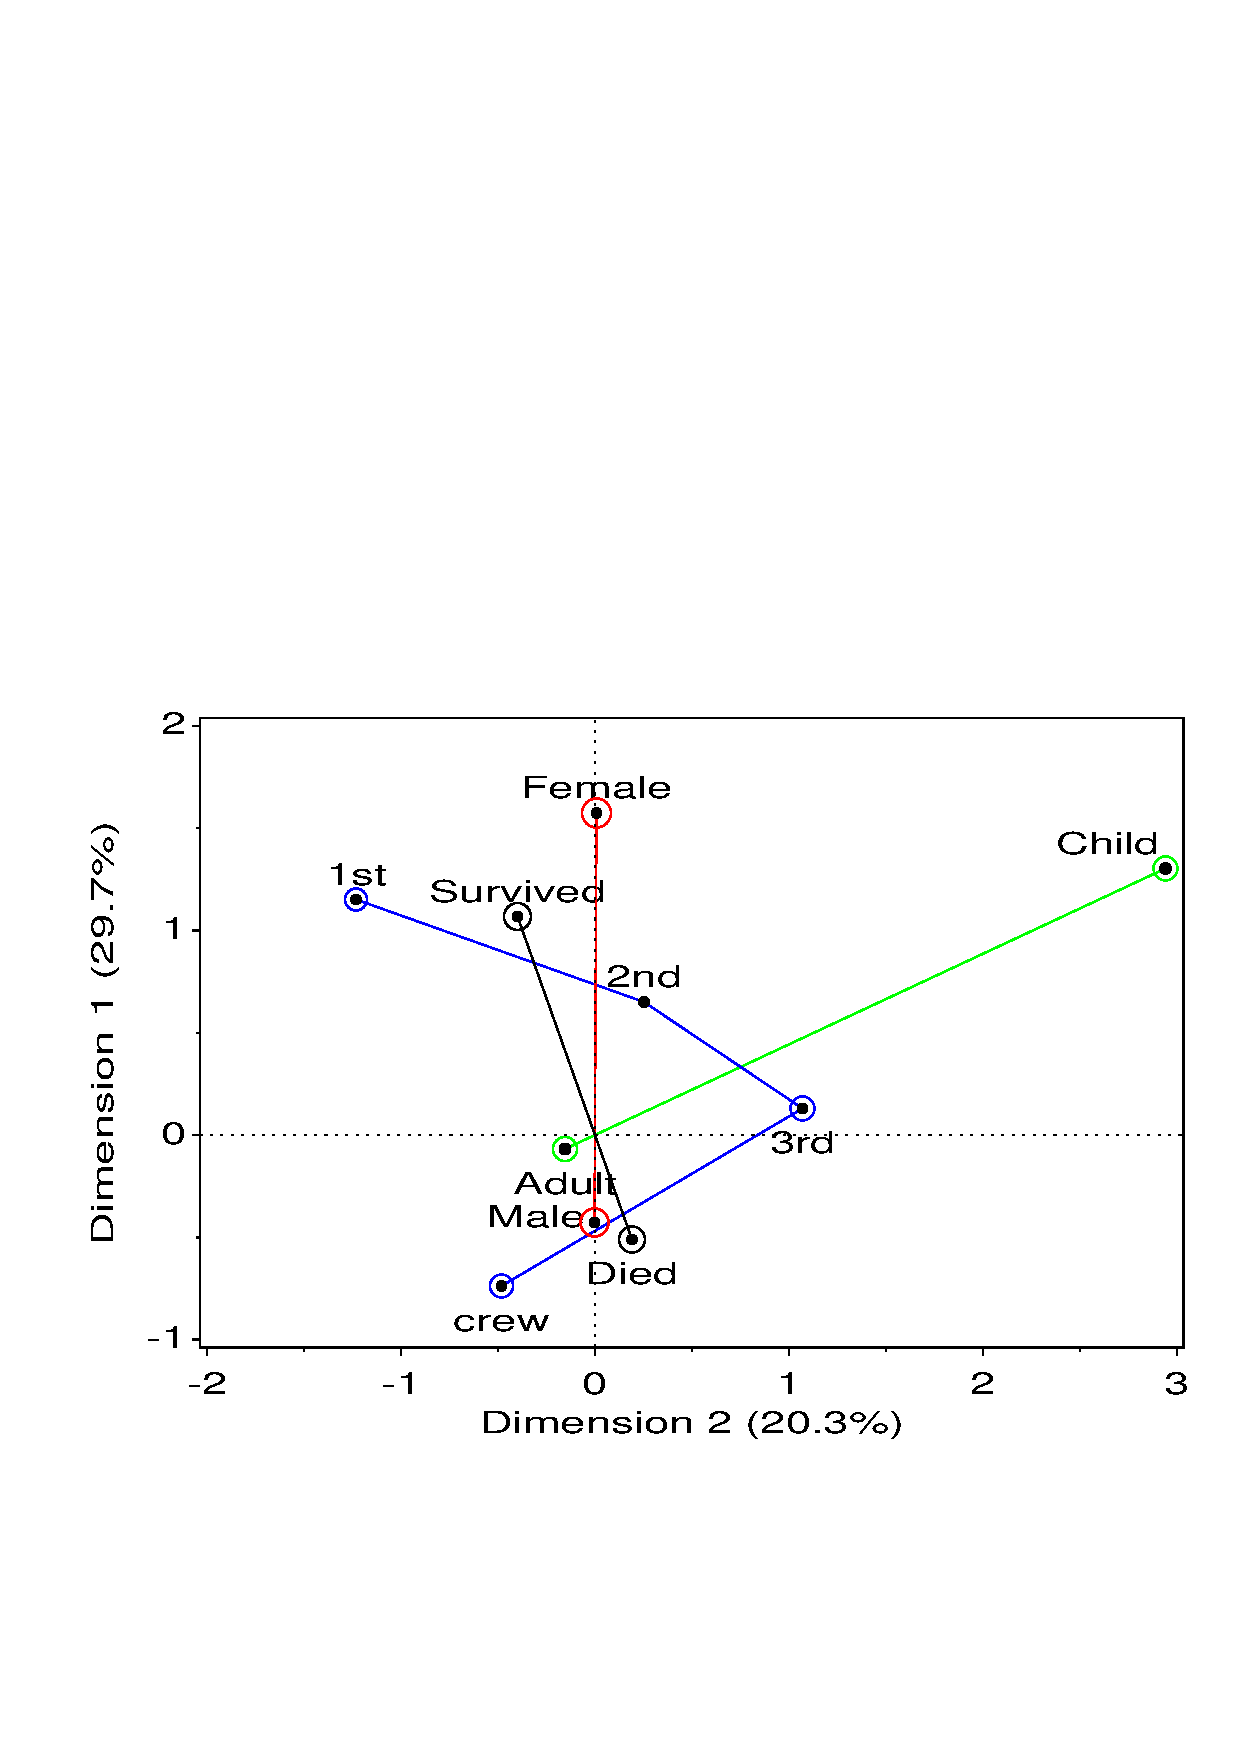
\includegraphics[scale=.8,clip]{ch5/fig/titanicmca}
  \caption{Titanic data: MCA analysis}\label{fig:titanicmca}
\end{figure}

%% input: /users/faculty/friendly/sasuser/catdata/titanicmca.sas
%% last modified: 04-Aug-98 17:16
\begin{listing}
data coords;
   set coords;
   where (_type_) = 'VAR';
   keep _name_ factor dim1-dim2 quality dist;
   dist = sqrt(dim1**2 + dim2**2);
   select;
      when (_name_ in ('Adult', 'Child'))   factor = 'Age    ';
      when (_name_ in ('Female', 'Male'))   factor = 'Sex    ';
      when (_name_ in ('Died', 'Survived')) factor = 'Survive';
      otherwise                             factor = 'Class';
      end;

proc sort;
   by factor;
proc print;
   id _name_;
%label(data=coords, x=dim2, y=dim1, text=_name_,
   pos=-, out=labels);

data labels;
   set labels;
   if text='Male' then do;
      x = x-.3;
      y = y+.2;
      end;

*-- join pairs of points representing the same variable;
data join;
   set coords;
   by factor;
   length function $8;
   xsys='2'; ysys='2';
   colors='green blue magenta red ';
   if first.factor then g+1;
   color = trim(scan(colors,g));
   x = dim2; y = dim1;
   if first.factor
      then function='move';
      else function='draw';
   output;
   *-- circle proportional to quality;
   size = .5 + 3*quality;
   text = 'circle';
   function = 'symbol';
   output;

data labels;           /* Concatenate the annotate data sets */
   set labels join;

title lspace=3.2in 'Survival on the Titanic';
proc gplot data=coords;
   plot dim1 * dim2 
      / frame href=0 vref=0 lvref=34 lhref=34
      vaxis=axis1 haxis=axis2 hm=1 vm=1
      anno=labels;
   symbol1 v=dot h=1;
   axis1 length=4.6in order=(-1 to 2) label=(a=90) ;
   axis2 length=7.65in order=(-2 to 3)  offset=(,.35in);
   label dim1 = 'Dimension 1 (29.7%)'
         dim2 = 'Dimension 2 (20.3%)';
   run;
\end{listing}


\begin{Output}[htb]
\caption{\CA\ coordinates for \emph{Titanic} MCA}\label{out:titanicmca2}
\begin{verbatim}
       _NAME_      QUALITY      DIM1        DIM2        DIST     FACTOR

       Adult       0.53947    -0.06783    -0.15332    0.16765    Age
       Child       0.53947     1.30180     2.94265    3.21774    Age
       1st         0.49259     1.15194    -1.23142    1.68623    Class
       2nd         0.07257     0.65126     0.25252    0.69850    Class
       3rd         0.54877     0.13060     1.07005    1.07799    Class
       crew        0.52193    -0.73694    -0.48273    0.88097    Class
       Female      0.67338     1.57479     0.00893    1.57482    Sex
       Male        0.67338    -0.42759    -0.00242    0.42759    Sex
       Died        0.61980    -0.50948     0.19024    0.54384    Survive
       Survived    0.61980     1.06768    -0.39867    1.13968    Survive
\end{verbatim}
\end{Output}

The mosaic matrix in \figref{fig:titanmos} may be compared with
the results of an MCA analysis of the \emph{Titanic} data.
\begin{figure}[!htb]
  \centering
  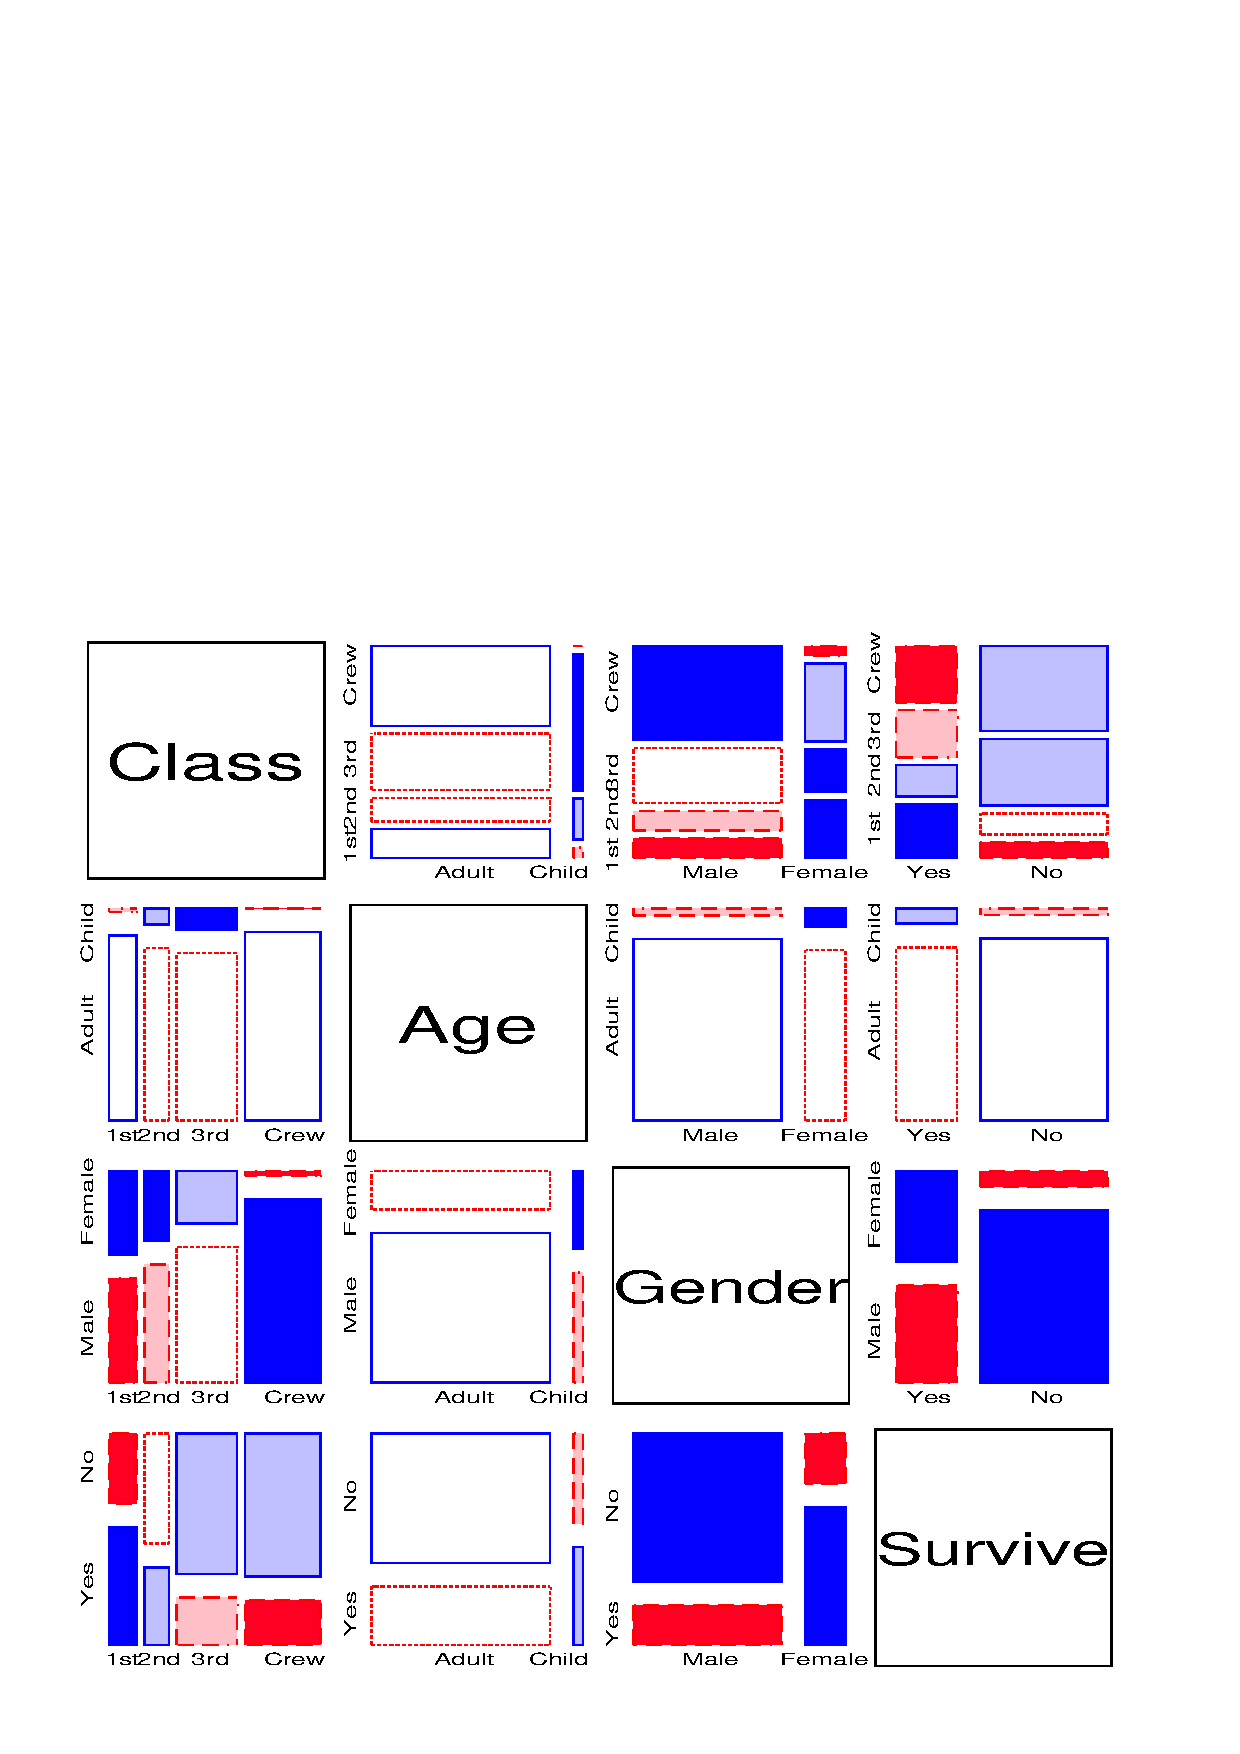
\includegraphics[scale=.7]{ch5/fig/titanmos}
  \caption[Mosaic matrix of \emph{Titanic} data]{Mosaic matrix of \emph{Titanic} data.  Each panel shows the marginal relation,
fitting an independence model between the row and column variable, collapsed over other variables.}\label{fig:titanmos}
\end{figure}
\end{Example}

\begin{Example}[marital3]{Marital status and pre- and extramarital sex}
The data on the relation between marital status and reported
premarital and extramarital sex was explored earlier using mosaic
displays in \exref{ex:marital1} and \exref{ex:marital2}.

The $2\times 2 \times 2 \times 2$ table in frequency form can be
analyzed as shown below, where the classification variables are
\pname{GENDER}, \pname{PRE}, \pname{EXTRA}, and \pname{MARITAL}.

\begin{listing}
data marital;
   input gender $ pre $ extra $ @;
    pre = 'Pre:' || pre;
    extra = 'X:' || extra;
   marital='Divorced';  input freq @;  output;
   marital='Married';   input freq @;  output;
datalines;
Women  Yes  Yes   17   4
Women  Yes  No    54  25
Women  No   Yes   36   4
Women  No   No   214 322
Men    Yes  Yes   28  11
Men    Yes  No    60  42
Men    No   Yes   17   4
Men    No   No    68 130
;

proc corresp data=marital mca outc=coords;
    weight freq;
    tables gender pre extra marital;
run;
\end{listing}
The same analysis, with the addition of the 2D plot of
category scores, would be produced by the \macro{CORRESP},
\begin{listing}
%corresp(data=marital, tables=gender pre extra marital, weight=freq, 
   options=mca short, interp=vec, inc=1, pos=-, symbols=dot);
\end{listing}

\begin{Output}[htb]
\caption{Chi-Square Decomposition for Marital status MCA}\label{out:maritalmca1}
\begin{output}
                      Inertia and Chi-Square Decomposition

        Singular  Principal Chi-                                        
        Values    Inertias  Squares Percents    8   16   24   32   40   
                                            ----+----+----+----+----+---
        0.62226   0.38721   1796.45  38.72% ************************    
        0.50915   0.25923   1202.70  25.92% ****************            
        0.43375   0.18814    872.86  18.81% ************                
        0.40672   0.16542    767.47  16.54% **********                  
                  -------   -------                                     
                  1.00000   4639.48 (Degrees of Freedom = 49)           
\end{output}
\end{Output}
%% one figure
\begin{figure}[htb]
  \centering
  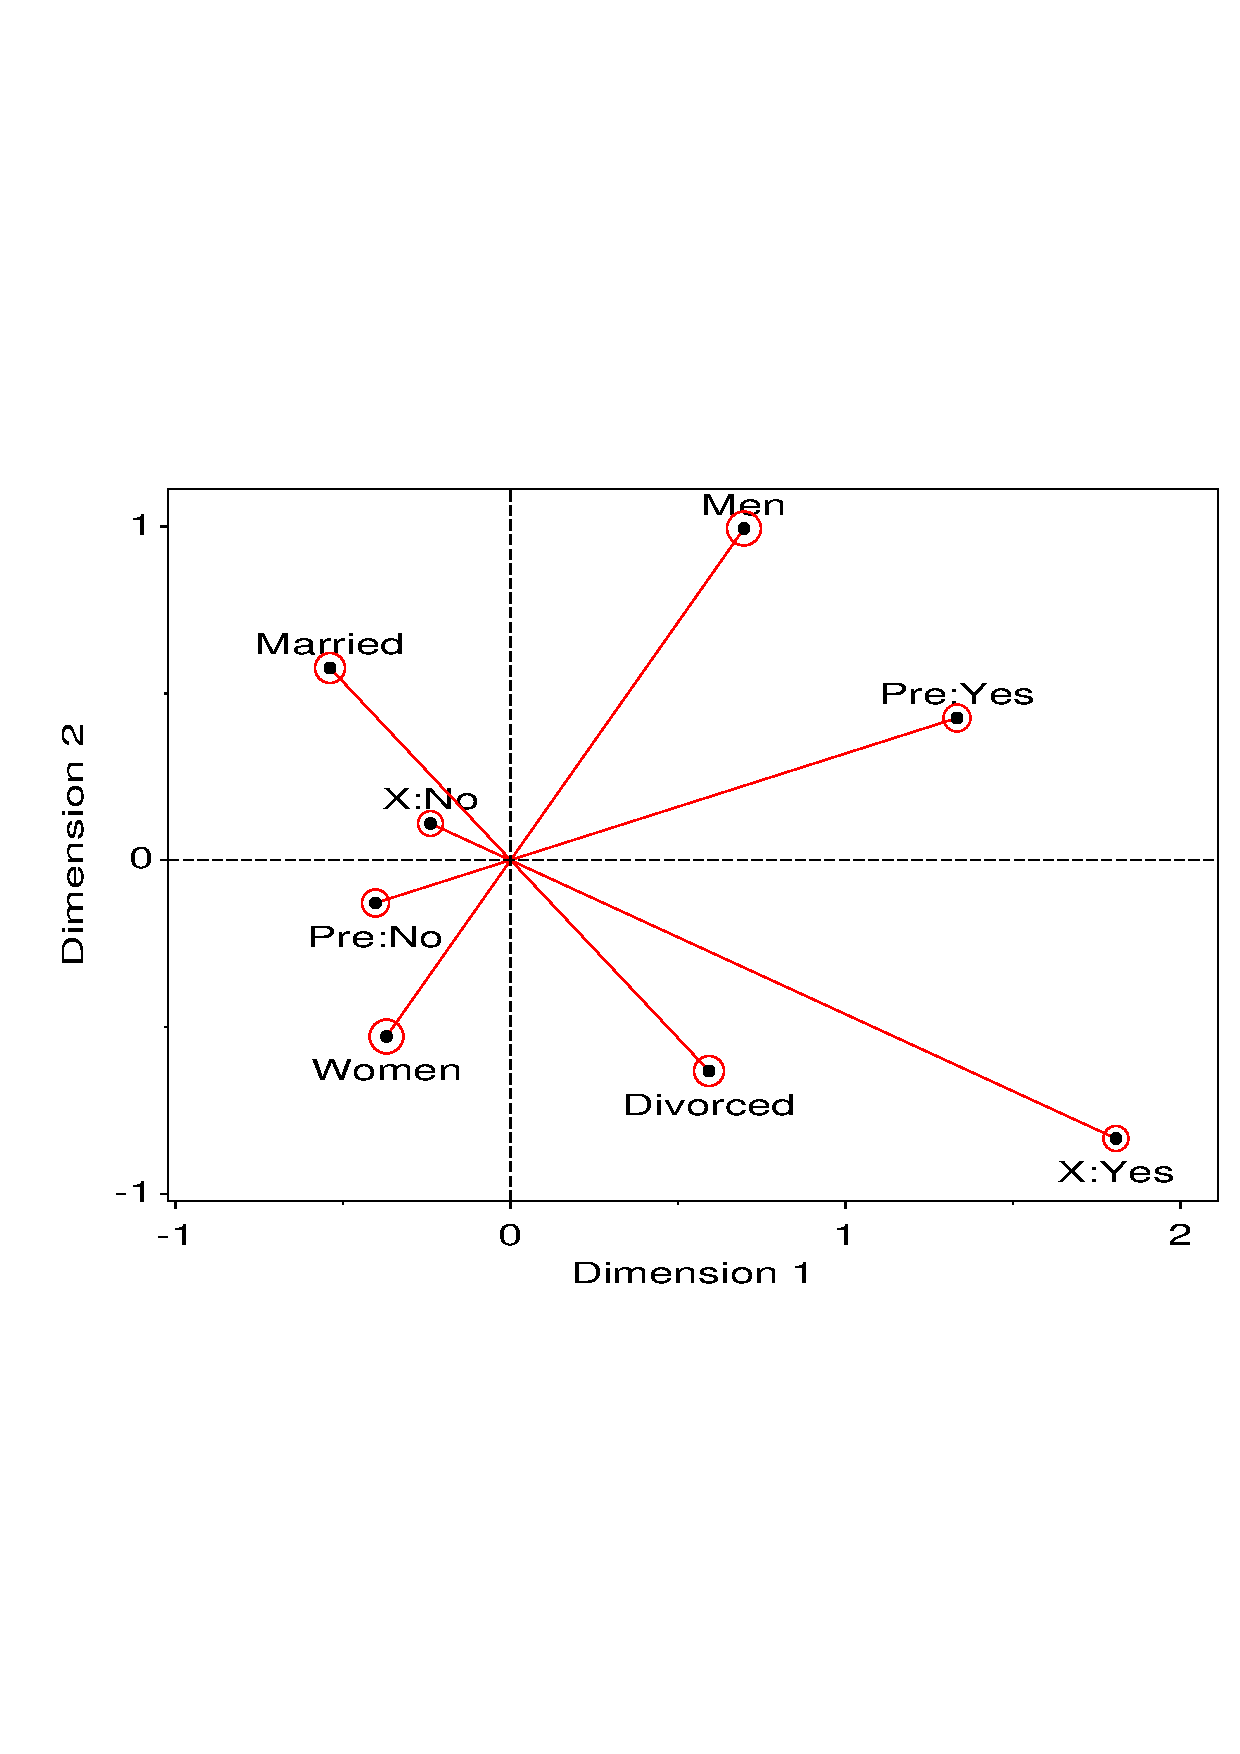
\includegraphics[scale=.8,clip]{ch5/fig/mcamarital1}
  \caption{2D multiple \CA\ display for marital status data}%
  \label{fig:mcamarital1}
\end{figure}

An enhanced version%
\footnote{The size of the bubble symbol surrounding each point is proportional
to the quality of the representation in two dimensions.}
of this plot is shown in \figref{fig:mcamarital1}.
The principal inertias, listed in \outref{out:maritalmca1}, again suggest
that two dimensions are sufficient for this \Dset.
The positions of the category points on Dimension 1 suggest that Women
are less likely to have had pre-marital and extra-marital sex
and that still being married is associated with the absence of pre- and extra-marital sex.

Although two dimensions are probably sufficient for interpreting these
data, we illustrate three-dimensional plots briefly.
When you specify the parameter \pname{DIM=3},
the \macro{CORRESP} produces a coordinates \Dset\ and an \ADS\
with three dimensions.%
\footnote{The first two dimensions are identical to the 2D solution,
because of the nested nature of CA and MCA solutions.}
It also produces a labeled \PROC{G3D} scatter plot.
However, the \pname{G3D} procedure does not allow axes to be equated,
and it is usually necessary to experiment with the \pname{ROTATE}
and \pname{TILT} options to produce a reasonable display, so the plot
generated by the macro should be considered just a first approximation.

A three-dimensional MCA solution for the Marital status data is produced with
this statement:
%% input: /Users/friendly/sasuser/catdata/mcamar.sas
%% last modified: 24-Jul-99 15:56
\begin{listing}
%corresp(data=marital, tables=gender pre extra marital, weight=freq, dim=3, 
   plotreq=dim1 * dim2 = dim3,
   options=mca short, interp=vec, symbols=dot,
   out=coord, anno=label);
\end{listing}
  

To roughly equate the axes,
the initial plot (not shown) was modified by extending the plotting range
for all dimensions as shown below.   Some additional annotation steps
(not shown) produces \figref{fig:mcamarital2}.  Note that the projections
of the points on the Dim1--Dim2 plane is identical to the solution shown
in \figref{fig:mcamarital1}.
%% input: /Users/friendly/sasuser/catdata/mcamar.sas
%% last modified: 21-Jul-99 11:19
\begin{listing}
data xtra;              /* Add dummy points to extend X, Y range */
   input dim1-dim3 shapevar $;
datalines;
 2   1  -.6  POINT
-1  -1  -.6  POINT
data coord;
   Set coord xtra;

goptions vsize=6in hsize=8in;
proc g3d data=coord;
   scatter dim1 * dim2 = dim3
      / shape='point' color='green'
        zmin=-0.6 tilt=80 rotate=75 caxis=gray60
        xticknum=2 yticknum=2 zticknum=2 grid
        annotate=label;
\end{listing}
  
\begin{figure}[htb]
  \centering
  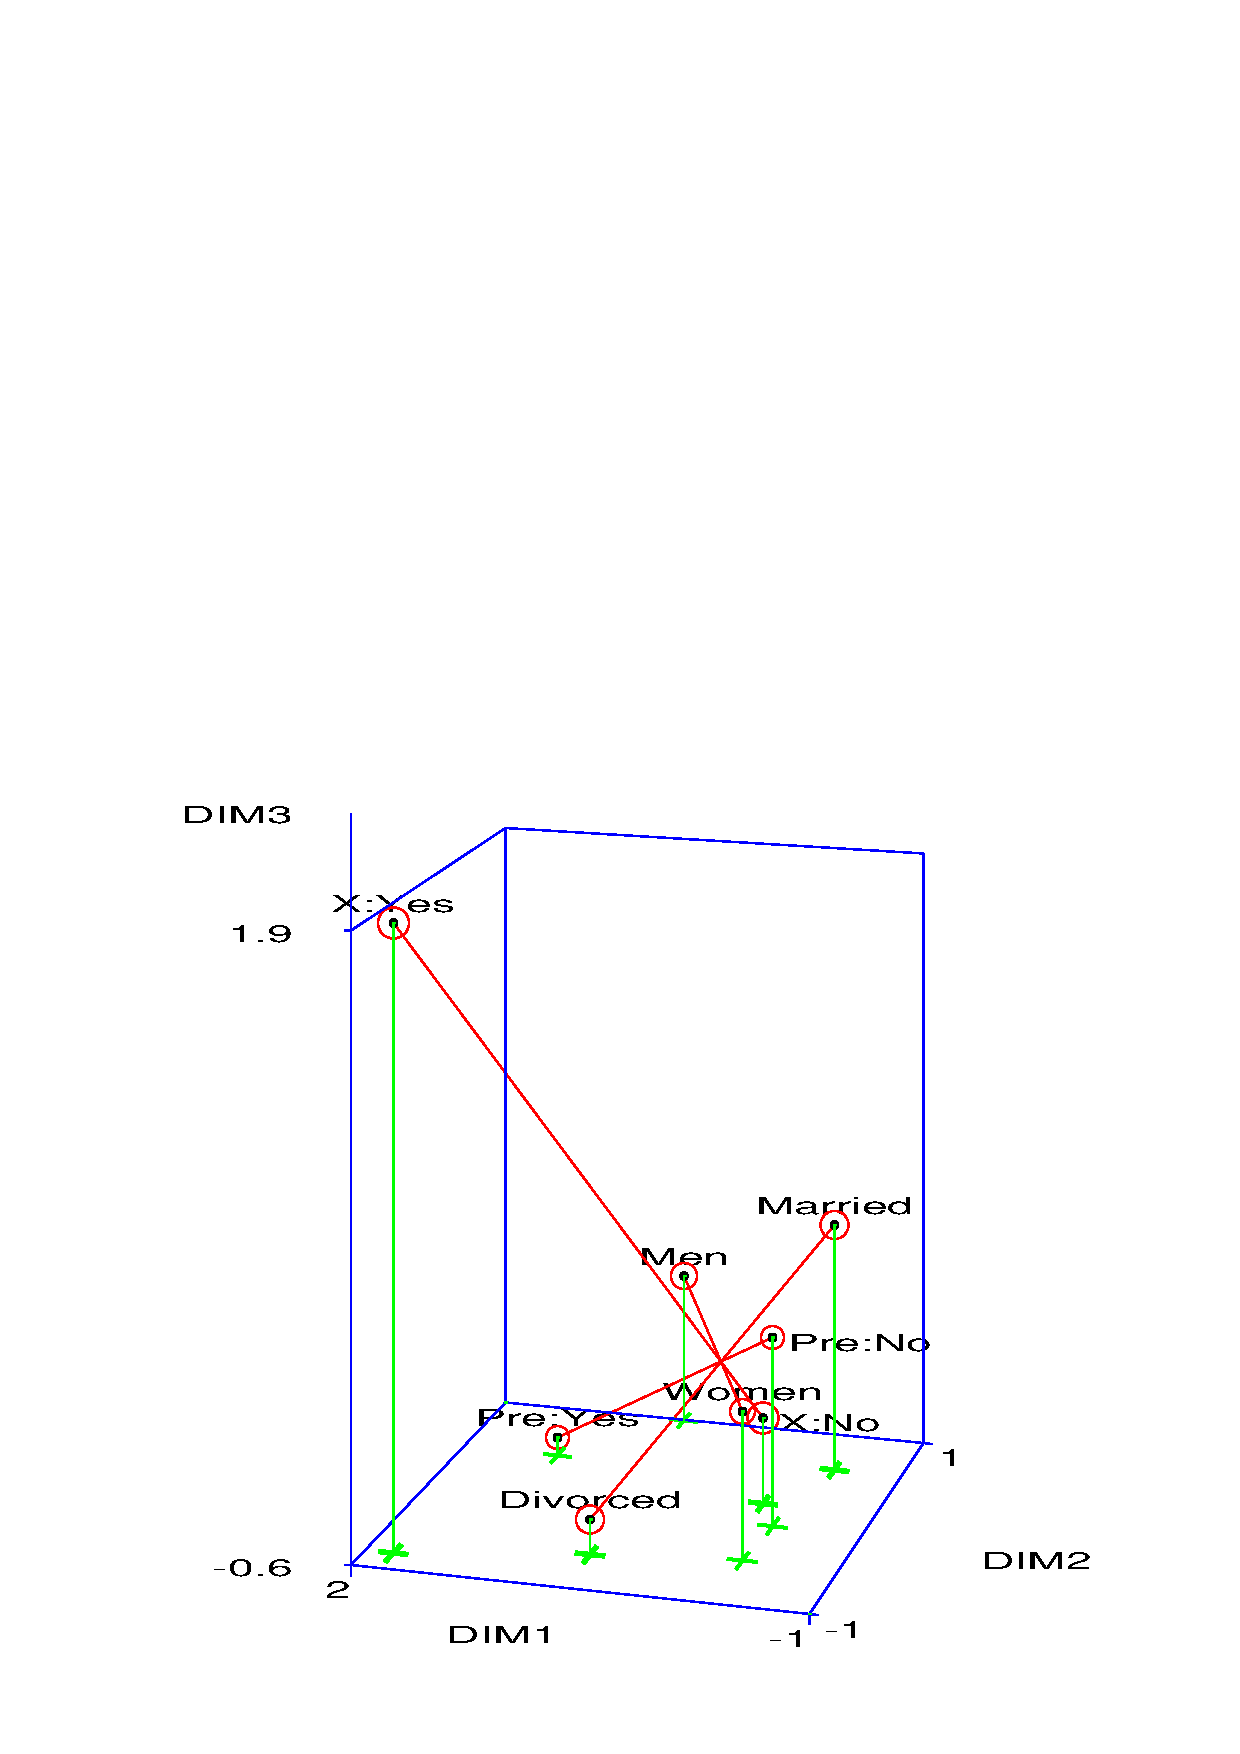
\includegraphics[scale=.8,clip]{ch5/fig/mcamarital2}
  \caption{3D multiple \CA\ display for marital status data}%
  \label{fig:mcamarital2}
\end{figure}
\end{Example}

\section{Extended MCA: Showing interactions in $2^Q$ tables}\label{sec:ca-mcainter}
\ixon{multiple correspondence analysis!extended}
As we discussed earlier,
MCA was developed as a way to depict the relationships among the
categories of multiple categorical variables, and the derivation of
the method based on the Burt matrix implies that only the relations
in the bivariate marginal tables are represented in the displays.
\ix{Burt matrix}
This is based on the assumption \citep{Gifi:90,Greenacre:88}
that, as with multivariate normal data, the structural relations
among variables are adequately captured by bivariate associations.%
\footnote{Another concern is that higher-way \ctab s may become
sparse, hence resulting in instability in solutions
\citep{Heijden:87}.}
These developments, and usually practice, have led to the mistaken beliefs that,
\begin{seriate}
\item MCA can \emph{only}
represent bivariate (first-order) interactions,
\item MCA can \emph{only} portray the category points of the variables
(not their combinations), and
\item associations must be inferred from the relative positions of
the category points.
\end{seriate}

A recent paper by \citet{MeulmanHeiser:97} demonstrates, however,
that none of these are necessary consequences of MCA itself.
Moreover, for the case of binary variables (a $2^Q$ table),
an odds interpretation of distances between category points
leads to simple geometrical patterns in MCA plots.

Their method for including higher-order effects involves adding all cross-terms,
up to a given order,
to the set of variables in frequency form which are analyzed by
MCA.  For example, with three variables, $A$, $B$, and $C$,
generate all interaction terms (using the \texttt{|} syntax of
\PROC{GLM} or \PROC{CATMOD}),
\begin{equation*}
\mbox{\texttt{A | B | C}} \iff \mbox{\texttt{A B C A*B A*C B*C A*B*C}}
\end{equation*}
\begin{table}[htb]
 \caption[Extended factor matrix for a $2\times 2\times2$ table]%
         {Extended factor matrix for a $2\times 2\times2$ table, including all possible cross-classifications.}\label{tab:mcadesign}\vspace{5pt}
\begin{center}
\begin{tabular}{lll | ccc ccc c}
 \hline
       &       &        &  A  &  B  &  C  &  AB &  AC &  BC & ABC \\ \hline
 $a_1$ & $b_1$ & $c_1$  &  1  &  1  &  1  &  1  &  1  &  1  &  1 \\
       &       & $c_2$  &  1  &  1  &  2  &  1  &  2  &  2  &  2 \\
       & $b_2$ & $c_1$  &  1  &  2  &  1  &  2  &  1  &  3  &  3 \\
       &       & $c_2$  &  1  &  2  &  2  &  2  &  2  &  4  &  4 \\
%
 $a_2$ & $b_1$ & $c_1$  &  2  &  1  &  1  &  3  &  3  &  1  &  5 \\
       &       & $c_2$  &  2  &  1  &  2  &  3  &  4  &  2  &  6 \\
       & $b_2$ & $c_1$  &  2  &  2  &  1  &  4  &  3  &  3  &  7 \\
       &       & $c_2$  &  2  &  2  &  2  &  4  &  4  &  4  &  8 \\
%
\end{tabular}
\end{center}
\end{table}

Similarly, the \texttt{@} syntax specifies all terms up to a given
order; for example,
\begin{equation*}
\mbox{\texttt{A | B | C | D}@2} \iff \mbox{\texttt{A B C D A*B A*C A*D B*C B*D C*D}}
\end{equation*}
generates all
terms up to order 2.  To illustrate, \tabref{tab:mcadesign} shows all terms
for the three-way model \texttt{(A | B | C)}.
Like any \pname{CLASS} variables, it is only necessary for the variable
values to be discrete.
However, it is strictly necessary to include \emph{all} terms at the same
interaction level, up to the given order.

The indicator matrix will then consist of the dummy variables for
these terms, so that, for \tabref{tab:mcadesign},
$\mat{Z} = [
 \mat{Z}_A  \mat{Z}_B  \mat{Z}_C  \mat{Z}_{AB}
 \mat{Z}_{AC}  \mat{Z}_{BC}  \mat{Z}_{ABC}
]$.
Forming the Burt matrix, $ \mat{B} =  \mat{Z}\trans  \mat{Z}$,
we see that the off-diagonal blocks now contain \emph{all}
contingency tables which can be formed from the original variables
(up to the specified order), not just the pairwise bivariate
tables.
The category points for an MCA solution based on this
extended $\mat{Z}$ matrix will then contain, in addition to the
usual one-way ``main effect'' points
of the variables themselves, sets of interaction points
(e.g., $(ab)_{ij}$, $(ac)_{ik}$, and so forth) for the various
combinations of factors included.

What happens to the category points for these interaction terms in the MCA
solution?
\citet{MeulmanHeiser:97} demonstrate the remarkable results that
\begin{itemize*}
\item distance ratios between sets of interaction points correspond to
odds ratios in the higher-order table,
and
\item the various independence structures we have considered
(cf. \tabref{tab:hyp3way})
give rise to simple configurations of points in the category
space.
\end{itemize*}

For simplicity, consider a $2\times 2$ table with cell probabilities
$p_{ij}$.  Let $\vec{z}_{ij}$
refer to the profile coordinate points for the $(ab)_{ij}$
combinations, and let $\vec{z}_{i\bullet}$, $\vec{z}_{\bullet j}$
be the coordinate points for the one-way $A$ and $B$ effects,
respectively.  Then, the  $\vec{z}_{ij}$ define a quadrilateral,
and the $\vec{z}_{i\bullet}$ and $\vec{z}_{\bullet j}$ are the
centroids (weighted by $p_{ij}$) of the corresponding corners,
as shown in \figref{fig:mcaidemo}.  In this figure, the mass, $p_{ij}$ of each cell point is indicated by its size and the $z$ points are labeled
by their subscripts.

\begin{figure}[htb]
  \centering
  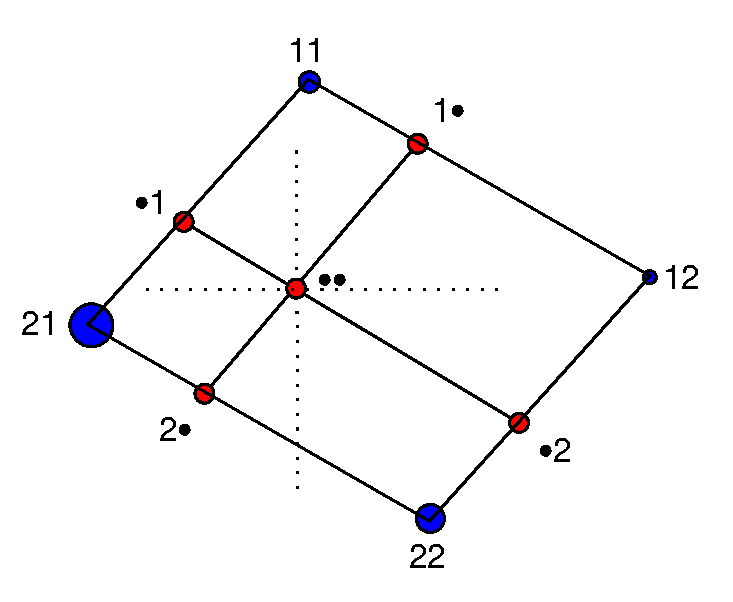
\includegraphics[scale=.9,clip]{ch5/fig/mcaidemo}
  \caption[Category points and profile points in extended MCA representation]{Category points ($\vec{z}_{ij}$) and profile points
  ($\vec{z}_{i\bullet}$, $\vec{z}_{\bullet j}$) in extended MCA representation. Under independence, the lines connecting the profile points are parallel to those connecting corresponding category points.}\label{fig:mcaidemo}
\end{figure}
The centroid points are related to the interaction points as (weighted)
linear combinations:
\begin{eqnarray*}%\label{eq:mcainter1}
  \vec{z}_{i \bullet} & = &
   \frac{p_{i1}}{p_{i+}} \: \vec{z}_{i1} +
   \frac{p_{i2}}{p_{i+}} \: \vec{z}_{i2} \\
  \vec{z}_{\bullet j} & = &
   \frac{p_{1j}}{p_{+j}} \: \vec{z}_{1j} +
   \frac{p_{2j}}{p_{+j}} \: \vec{z}_{2j}
\end{eqnarray*}
Now, for any edge of the quadrilateral, e.g., $z_{i1}$, $z_{i2}$,
their centroid is located on the line between them, so the
distances must be additive,
\begin{equation*}%\label{eq:mcainter2}
  d( \vec{z}_{i1}, \vec{z}_{i2} ) =
  d( \vec{z}_{i1}, \vec{z}_{i \bullet} ) +
  d( \vec{z}_{i \bullet}, \vec{z}_{i2} )
\end{equation*}
From these relations, \citet{MeulmanHeiser:97} show that:
\begin{itemize}
\item Given $A=i$ (or, $B=j$), the odds of being in category 1 vs. category 2
of $B$ (or $A$) are shown in the display by the inverse ratio of their
distances to their centroid.  For example,
\begin{equation*}%\label{eq:mcainter3}
  \frac{p_{i1}}{p_{i2}} =
  \frac{ d( \vec{z}_{i2}, \vec{z}_{i \bullet} ) }
       { d( \vec{z}_{i1}, \vec{z}_{i \bullet} ) }
\end{equation*}
\item The odds ratio $\theta$ has a simple multiplicative relation
to these distances among the four corner points and their
centroids.
\begin{equation}\label{eq:mcainter4}
  \theta =
  \frac{p_{11} p_{22}}{p_{12} p_{21}} =
  \frac{ d( \vec{z}_{12}, \vec{z}_{\bullet 2}) \: d( \vec{z}_{21}, \vec{z}_{\bullet 1} )}
       { d( \vec{z}_{11}, \vec{z}_{\bullet 1}) \: d( \vec{z}_{22}, \vec{z}_{\bullet 2} )}
\end{equation}
\item Under independence, $\theta =1$, and \eqref{eq:mcainter4}
therefore implies that
(a) the corner points form a parallelogram, and
(b) the lines connecting the centroids of the same variable
(e.g., $(\vec{z}_{\bullet 1}, \vec{z}_{\bullet 2}))$ are parallel
to those of their respective category points.
These relations of parallelism and additivity are shown in \figref{fig:mcaidemo}.
\end{itemize}

Although this discussion was presented
in terms of a $2 \times 2$ table, the geometrical relations extend
directly to \emph{any} number of binary variables.
For a $2 \times 2 \times 2$ table,  the models of various types of
independence shown in \tabref{tab:hyp3way} can all be characterized
in terms of the three odds ratios for all pairs of variables, and
therefore in terms of parallelism and additivity of the corresponding
pairwise quadrilaterals in the spatial representation.
Essentially, each independence relation corresponds to one odds ratio $\theta=1$,
which in turn is shown as one two-way term whose profile points form
a parallelogram, as shown in the table below.
 \begin{center}
 \begin{tabular}{lll c}
 \hline
            &  Independence  &             &  Number of parallel    \\
Hypothesis  &  relations     & Odds ratios &  two-way profile sets  \\ \hline
$H_1$  & $A \perp B \perp C$ &  $\theta_{AB} = \theta_{AC} = \theta_{BC} = 1$ & 3 \\
%
$H_2$  & $A , B \perp C$     &  $\theta_{AC} = \theta_{BC} = 1$ & 2 \\
%
$H_3$  & $A \perp B \given C$ &  $\theta_{AB} = 1$               & 1 \\
%
$H_4$  & none                & all $\theta \neq 1$               & 0 \\
%
  \hline
 \end{tabular}
 \end{center}


The following example demonstrates these ideas with a $2^3$ table, where
one two-way term is independent by design.
It also illustrates how to generate the interaction
variables, and some special techniques for displaying the extended
MCA solution.

\begin{Example}[bartlett]{Bartlett's data}
In a classic paper that extended the notion of interaction to three-way
tables, \citet{Bartlett:35} gave the data shown in \tabref{tab:bartlett}
from an experiment designed to investigate the propagation of
plum root stocks from cuttings.
In the $2 \times 2 \times 2$ table, time of planting (T) and length
of cutting (L) are factors; whether the cutting was alive or dead (A)
was the response.
Note that the column totals for the factors are all equal,
these having been fixed by the experimental design.
Thus, there can be
no $T\times L$ marginal association, and interest naturally is focused
on the [AT] and [AL] associations.
%%
%% Table bartlett written by md2tex 13AUG98 12:17
%%
\begin{table}[htb]
 \caption{Bartlett's data on propagation of plum root stocks}
 \label{tab:bartlett}
 \begin{center}
  \begin{tabular}{|l|rrrr|r|}
   \hline
 & \multicolumn{4}{c|}{\bfseries\large Time of planting} & \rule{0in}{2.5ex}\\
 & \multicolumn{2}{c|}{Now   } & \multicolumn{2}{c|}{Spring} &  \\\cline{2-5}
 & \multicolumn{4}{c|}{\bfseries\large Length of cutting} & \rule{0in}{2.5ex}\\
{\bfseries\large Alive?} & Long   & Short  & Long   & Short & {\bfseries\large Total} \\
   \hline
Alive    &      156 &      107 &       84 &       31 &      378 \\
Dead     &       84 &      133 &      156 &      209 &      582 \\
   \hline
\rule{0in}{2.5ex}{\bfseries\large Total} &     240 &      240 &      240 &      240 &      960 \\
   \hline
  \end{tabular}
 \end{center}
\end{table}


The marginal relations are easily seen in a mosaic matrix, shown in
\figref{fig:mosmat1m}. Time and Length are independent, but
there is a strong [AT] association, with planting
now more likely to be successful, and a weaker [AL] association,
so that long cutting are more likely to survive.

\begin{figure}[htb]
  \centering
  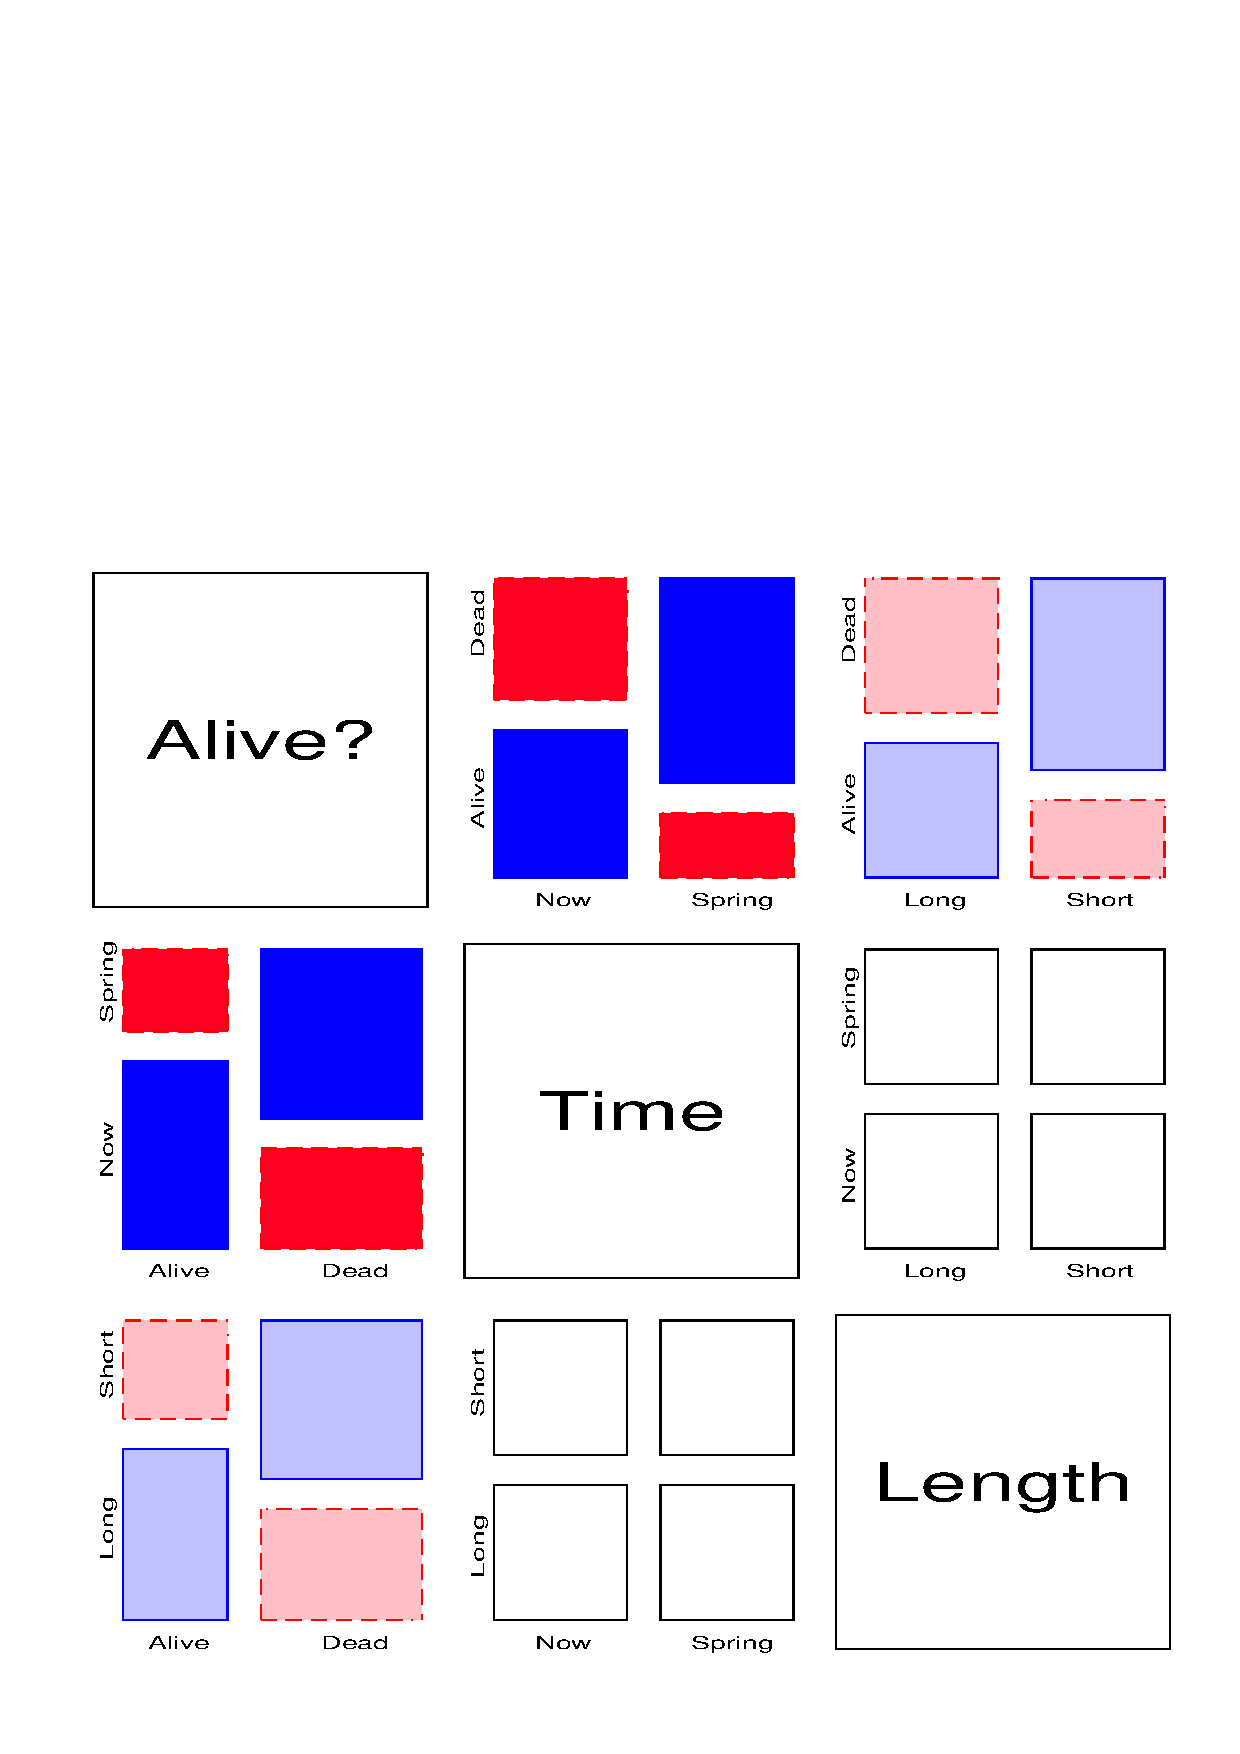
\includegraphics[scale=.7,clip]{ch5/fig/mosmat1m}
  \caption{Mosaic matrix for marginal associations in Bartlett's data}\label{fig:mosmat1m}
\end{figure}
The standard MCA analysis is carried out with the statements below.
In the call to the \macro{CORRESP}, the \mparm{INTERP=VEC}{CORRESP}
draws vectors from the origin to each main category point.
The macro produces the graph of the 2D solution shown in \figref{fig:mcabart1}; the principal inertias are shown in
\outref{out:mcabart1}.
%% input: /Users/friendly/sasuser/catdata/mcabart.sas
%% last modified: 26-Jul-99 10:48
\begin{listing}
data bartlett;
   do alive='Alive', 'Dead';
      do time='Now   ', 'Spring';
         do Length = 'Long ', 'Short';
            input count @;
            output;
            end;
         end;
      end;
datalines;
 156 107  84  31
  84 133 156 209
;
*-- Ordinary MCA of the three variables;
%corresp(data=bartlett, tables=Alive Time Length, weight=count,
   options=mca short, interp=vec, inc=0.2, pos=-,
   symbols=dot, colors=black, m0=0);
\end{listing}


\begin{figure}[htb]
  \centering
  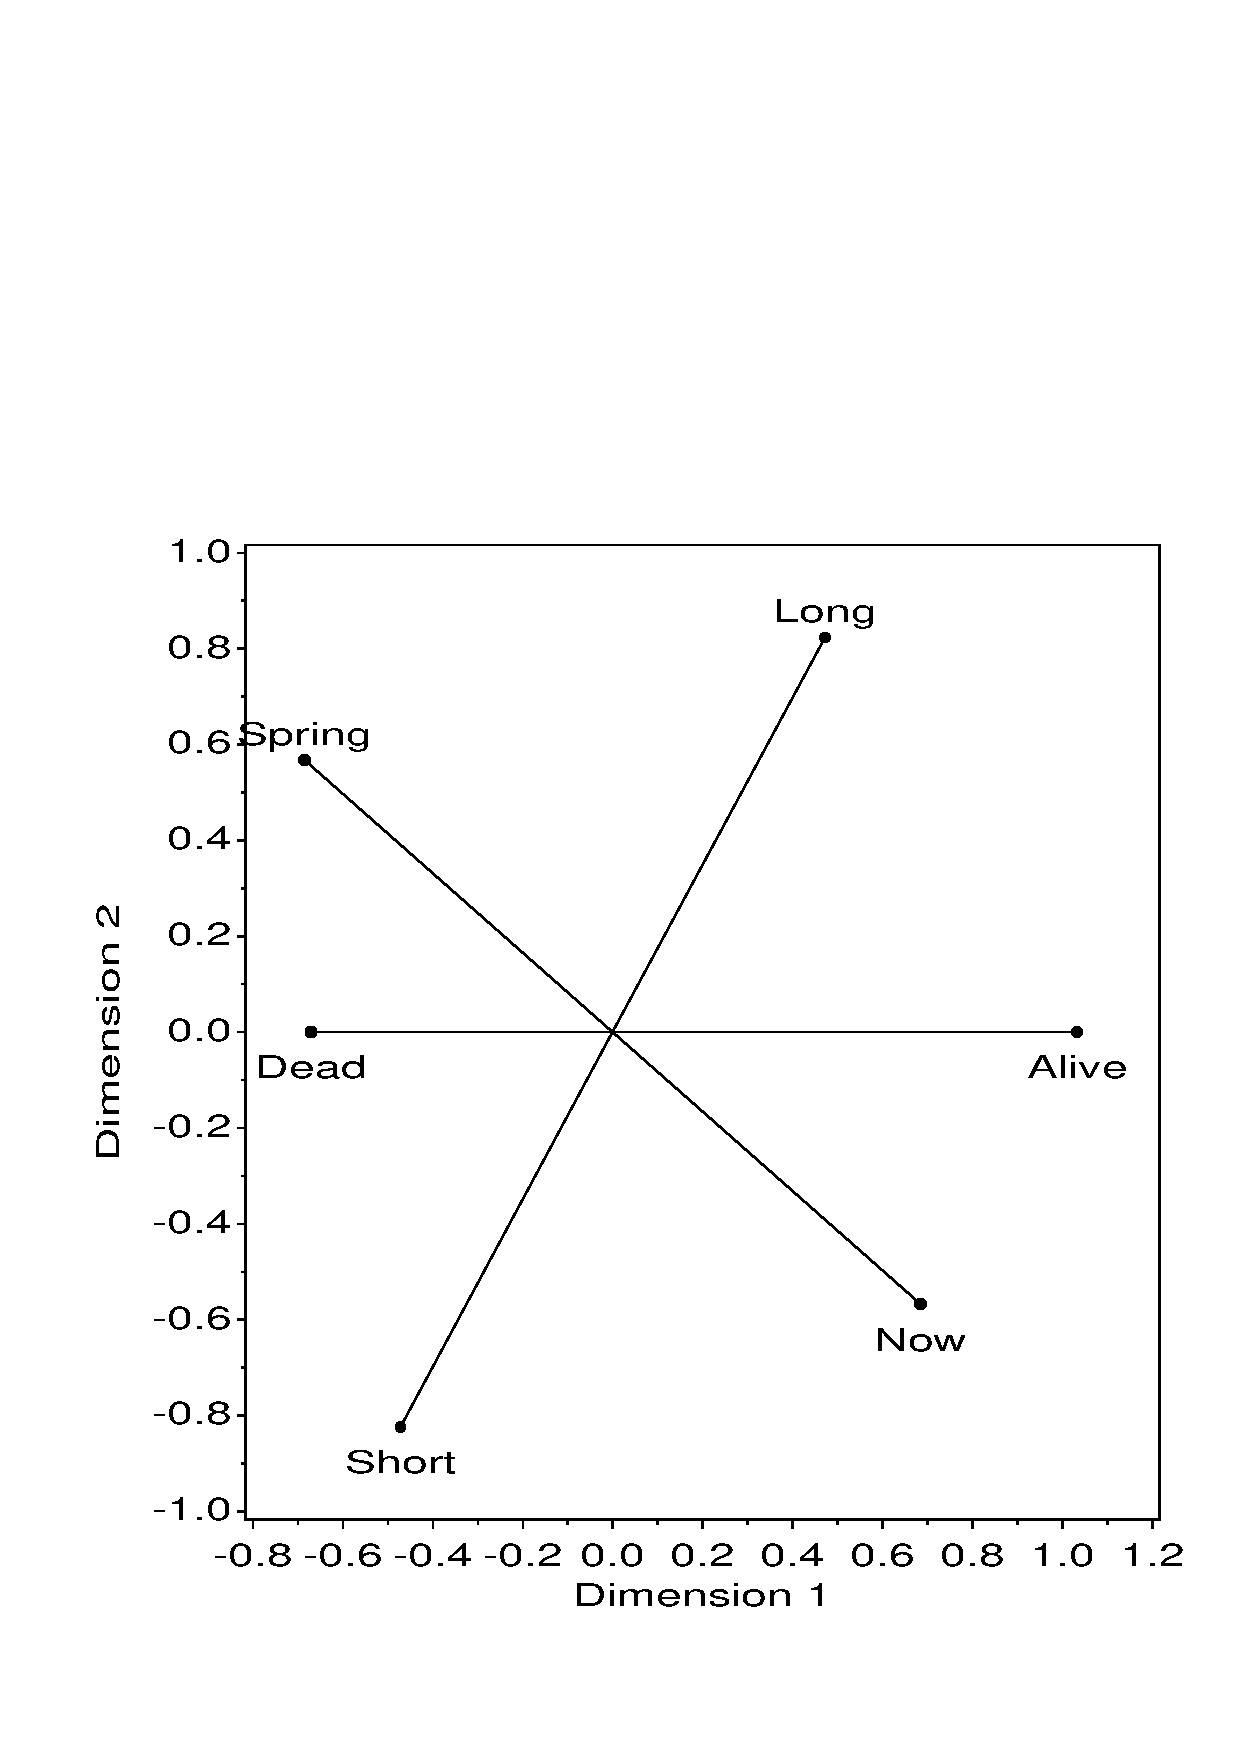
\includegraphics[scale=.7,clip]{ch5/fig/mcabart1}
  \caption{2D MCA solution for Bartlett's data}\label{fig:mcabart1}
\end{figure}

The interpretation of \figref{fig:mcabart1} is quite simple.
Dimension 1 is perfectly aligned with the Alive response variable.
The associations [AT] and [AL] of Time and Length are shown by their projections
(coordinates) on this axis.
Time has a stronger association, so its projection on this axis is larger,
and planting Long cuttings, Now leads to increased survival.
The independence of Time and Length is shown by the nearly
right angle between their vectors.%
\footnote{In an equated 3D representation, they \emph{are} orthogonal.}
Because the second principal inertia in \outref{out:mcabart1}
equals $1/Q = 1/3$ we do not interpret the second dimension.
\begin{Output}[htb]
\caption{Chi-Square Decomposition for Bartlett's data, MCA}\label{out:mcabart1}
\begin{output}
                      Inertia and Chi-Square Decomposition

        Singular  Principal Chi-
        Values    Inertias  Squares Percents    9   18   27   36   45
                                            ----+----+----+----+----+---
        0.67902   0.46107   1457.90  46.11% **************************
        0.57735   0.33333   1053.99  33.33% *******************
        0.45342   0.20559    650.08  20.56% ***********
                  -------   -------
                  1.00000   3161.97 (Degrees of Freedom = 25)
\end{output}
\end{Output}
Note also how the odds are shown by distance ratios in the plot.
Both Time and Length have equal marginal frequencies for their two
levels (odds = 1), and the ratio of distances to the origin for
the levels of both variables equals 1.0.
The ratio of distances to the origin for Alive and Dead
is inversely related to their marginal frequencies.

The statements below illustrate one way to construct the interaction
variables representing the first-order associations [AT], [AL], and [TL]
and the second-order interaction, [ATL].
Each of the character variables \pname{ALIVE}, \pname{TIME},
and \pname{LENGTH} is used to create a dummy (0/1) variable
(\pname{A}, \pname{T}, and \pname{L}, respectively).
The interaction terms are then created with binary arithmetic
in the \Dstp\ \pname{COMBO}.
A \PROC{FORMAT} step is used to create short character labels for the
combinations, to be used in the plots which follow.
These labels use an upper case letter to refer to the first level of
each main variable and a lower case letter to refer to the second level.

The \Dset\ \pname{COMBO} which results is shown in \outref{out:mcabart2}.
Note that the variables \pname{A--ATL} are actually numeric, but are printed
using their formatted values.%
\footnote{Because the interaction
variables need only be discrete, they could be created more easily, simply
by concatenating the main variables,
(e.g., \texttt{AT = ALIVE || TIME;}, and so forth).  This would produce
cluttered displays, however, because each combination is plotted and labeled.}
%
%% input: /users/faculty/friendly/sasuser/catdata/mcabart.sas
%% last modified: 13-Aug-98 17:34
\begin{listing}
*-- Formats for higher-order effects;
proc format;
   value a  0='a' 1='A';
   value t  0='t' 1='T';
   value l  0='l' 1='L';
   
   value at 0='at' 1='aT' 2='At' 3='AT';
   value al 0='al' 1='aL' 2='Al' 3='AL';
   value tl 0='tl' 1='tL' 2='Tl' 3='TL';
   value atl 0='atl' 1='atL' 2='aTl' 3='aTL' 4='Atl' 5='AtL' 6='ATl' 7='ATL';

*-- Code combinations of variables;
data combo;
   set bartlett;
   
   a = (alive='Alive');
   t = (time='Now');
   l = (length='Long');
   
   at = 2*a + t;
   al = 2*a + l;
   tl = 2*t + l;
   
   atl = 4*a + 2*t + l;
   format a a. t t. l l.  at at.  al al.  tl tl.  atl atl.;
proc print noobs;

\end{listing}

\begin{Output}[htb]
\caption{\Dset\ \pname{COMBO}: Interactive coding for Bartlett's data, Extended MCA}\label{out:mcabart2}
\begin{output}
   LENGTH    TIME      ALIVE    COUNT    A    T    L    AT    AL    TL    ATL

   Long      Now       Alive     156     A    T    L    AT    AL    TL    ATL
   Long      Now       Dead       84     a    T    L    aT    aL    TL    aTL
   Long      Spring    Alive      84     A    t    L    At    AL    tL    AtL
   Long      Spring    Dead      156     a    t    L    at    aL    tL    atL
   Short     Now       Alive     107     A    T    l    AT    Al    Tl    ATl
   Short     Now       Dead      133     a    T    l    aT    al    Tl    aTl
   Short     Spring    Alive      31     A    t    l    At    Al    tl    Atl
   Short     Spring    Dead      209     a    t    l    at    al    tl    atl
\end{output}
\end{Output}

Applying MCA to this \Dset\ using the main effect variables \pname{A T L}
would produce results identical to \figref{fig:mcabart1}.
Adding the three two-way variables, \pname{AT AL TL} will add $3 \times 4$
category points for the pairwise combinations of these factors.
The three-way variable, \pname{ATL}, adds an additional
8 category points, representing the individual cells in the table.

The analysis shown below excludes the three-way \pname{ATL} terms for simplicity.
As long as the terms are added in a balanced way
(including all terms of a given order), the positions of points tend to be very
similar whether or not terms of higher-order are included.

%% input: /users/faculty/friendly/sasuser/catdata/mcabart.sas
%% last modified: 16-Aug-98 12:26
\begin{listing}
proc corresp data=combo  mca outc=coords short;
   weight count;
   tables a t l at al tl;* atl;

*-- Identify the size and name of each effect;
data coords;
   set coords;
   where (_type_) = 'VAR';
   drop _type_ inertia contr1--best;
   terms=length(_name_);
   effect = upcase(_name_);
   label dim1 = 'Dimension 1'
         dim2 = 'Dimension 2';
proc sort;
   by terms effect _name_;
proc print;
   id _name_ effect terms;
   var dim1 dim2 mass;
\end{listing}

The \ODS\ \pname{COORDS} is used to produce the plots
shown in \figref{fig:mcabart2}.
In order to draw the vectors for the main effect points,
and quadrilaterals for the two-way terms
as in \figref{fig:mcaidemo}, variables \pname{TERMS} and \pname{EFFECT}
are added to the \pname{COORDS} \Dset\ as shown above.

%% two subfig side-by-side
\begin{figure}[htb]
 \begin{minipage}[t]{.49\linewidth}
  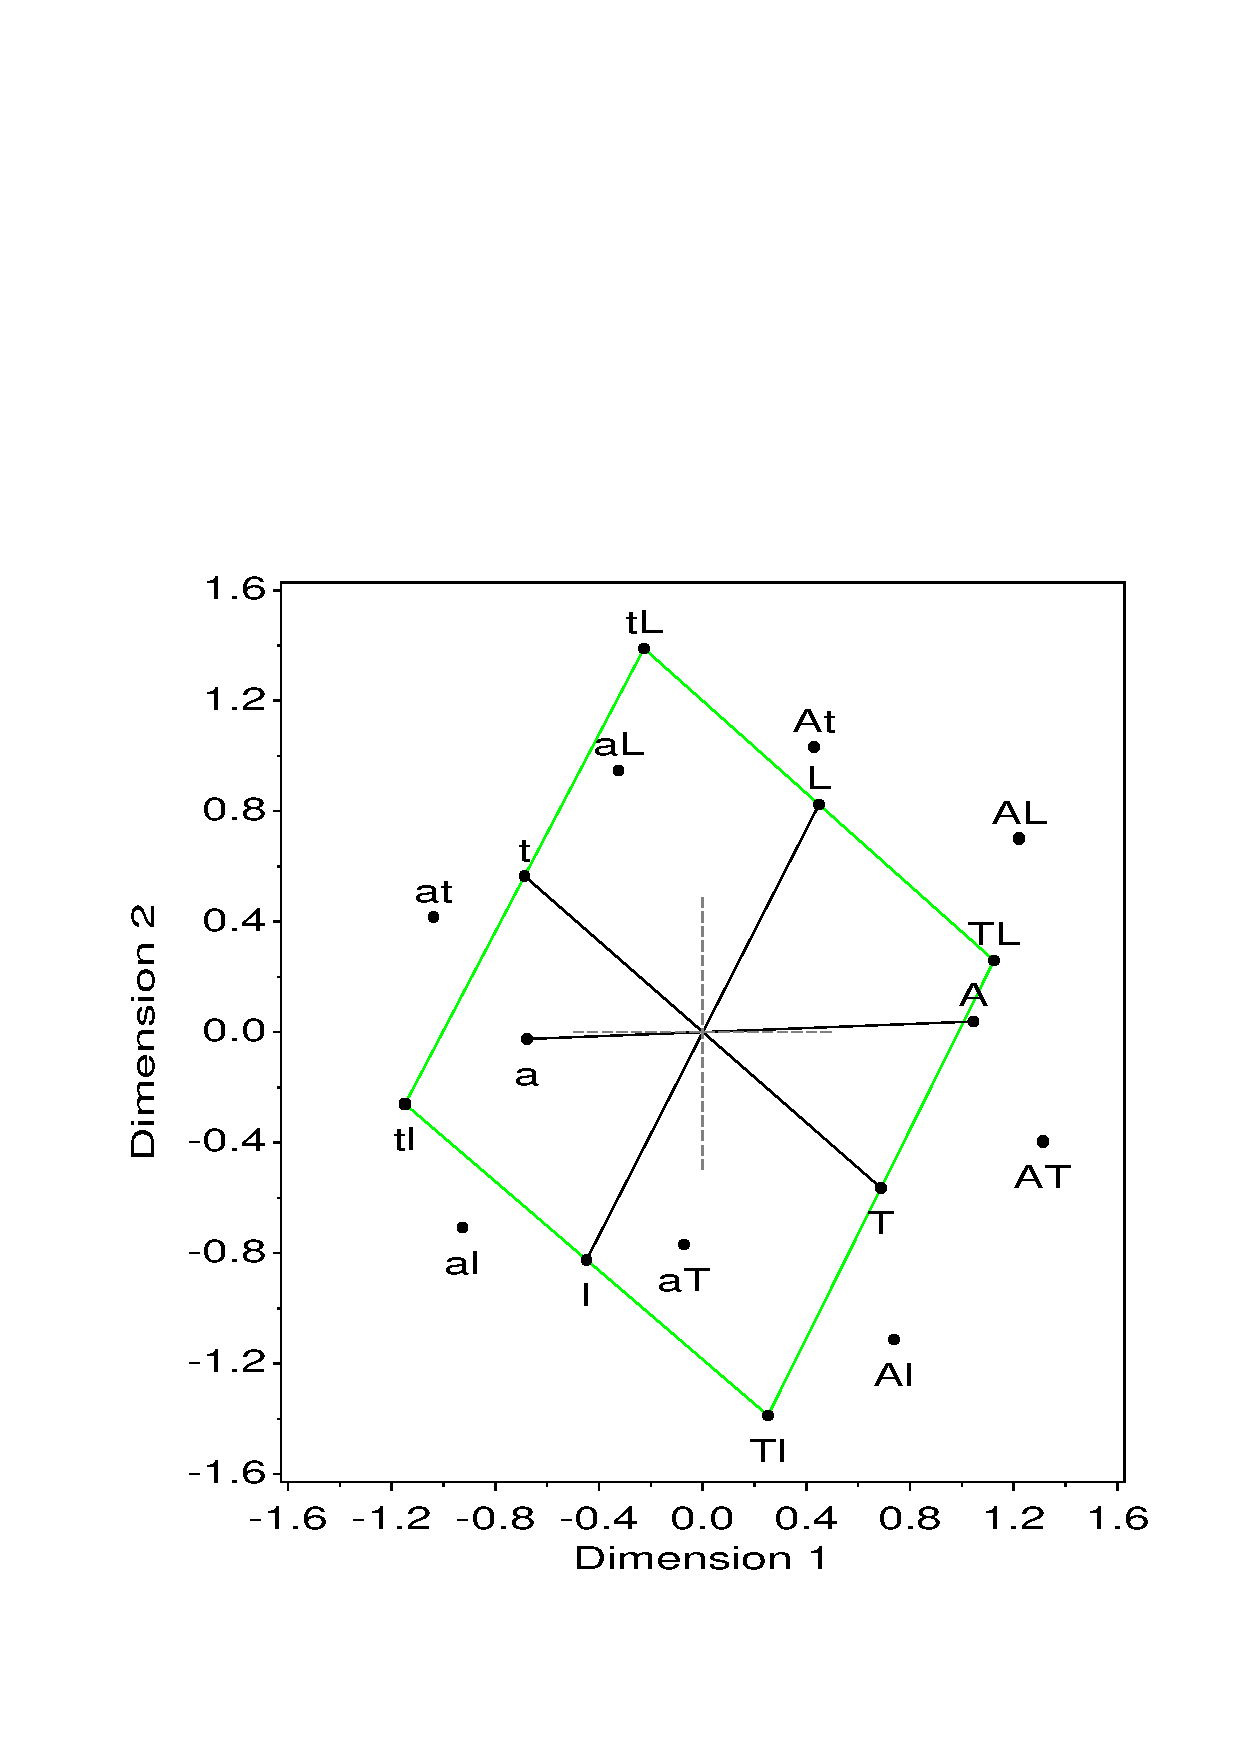
\includegraphics[width=1\linewidth]{ch5/fig/mcabart2}
 \end{minipage}%
 \hfill
 \begin{minipage}[t]{.49\linewidth}
  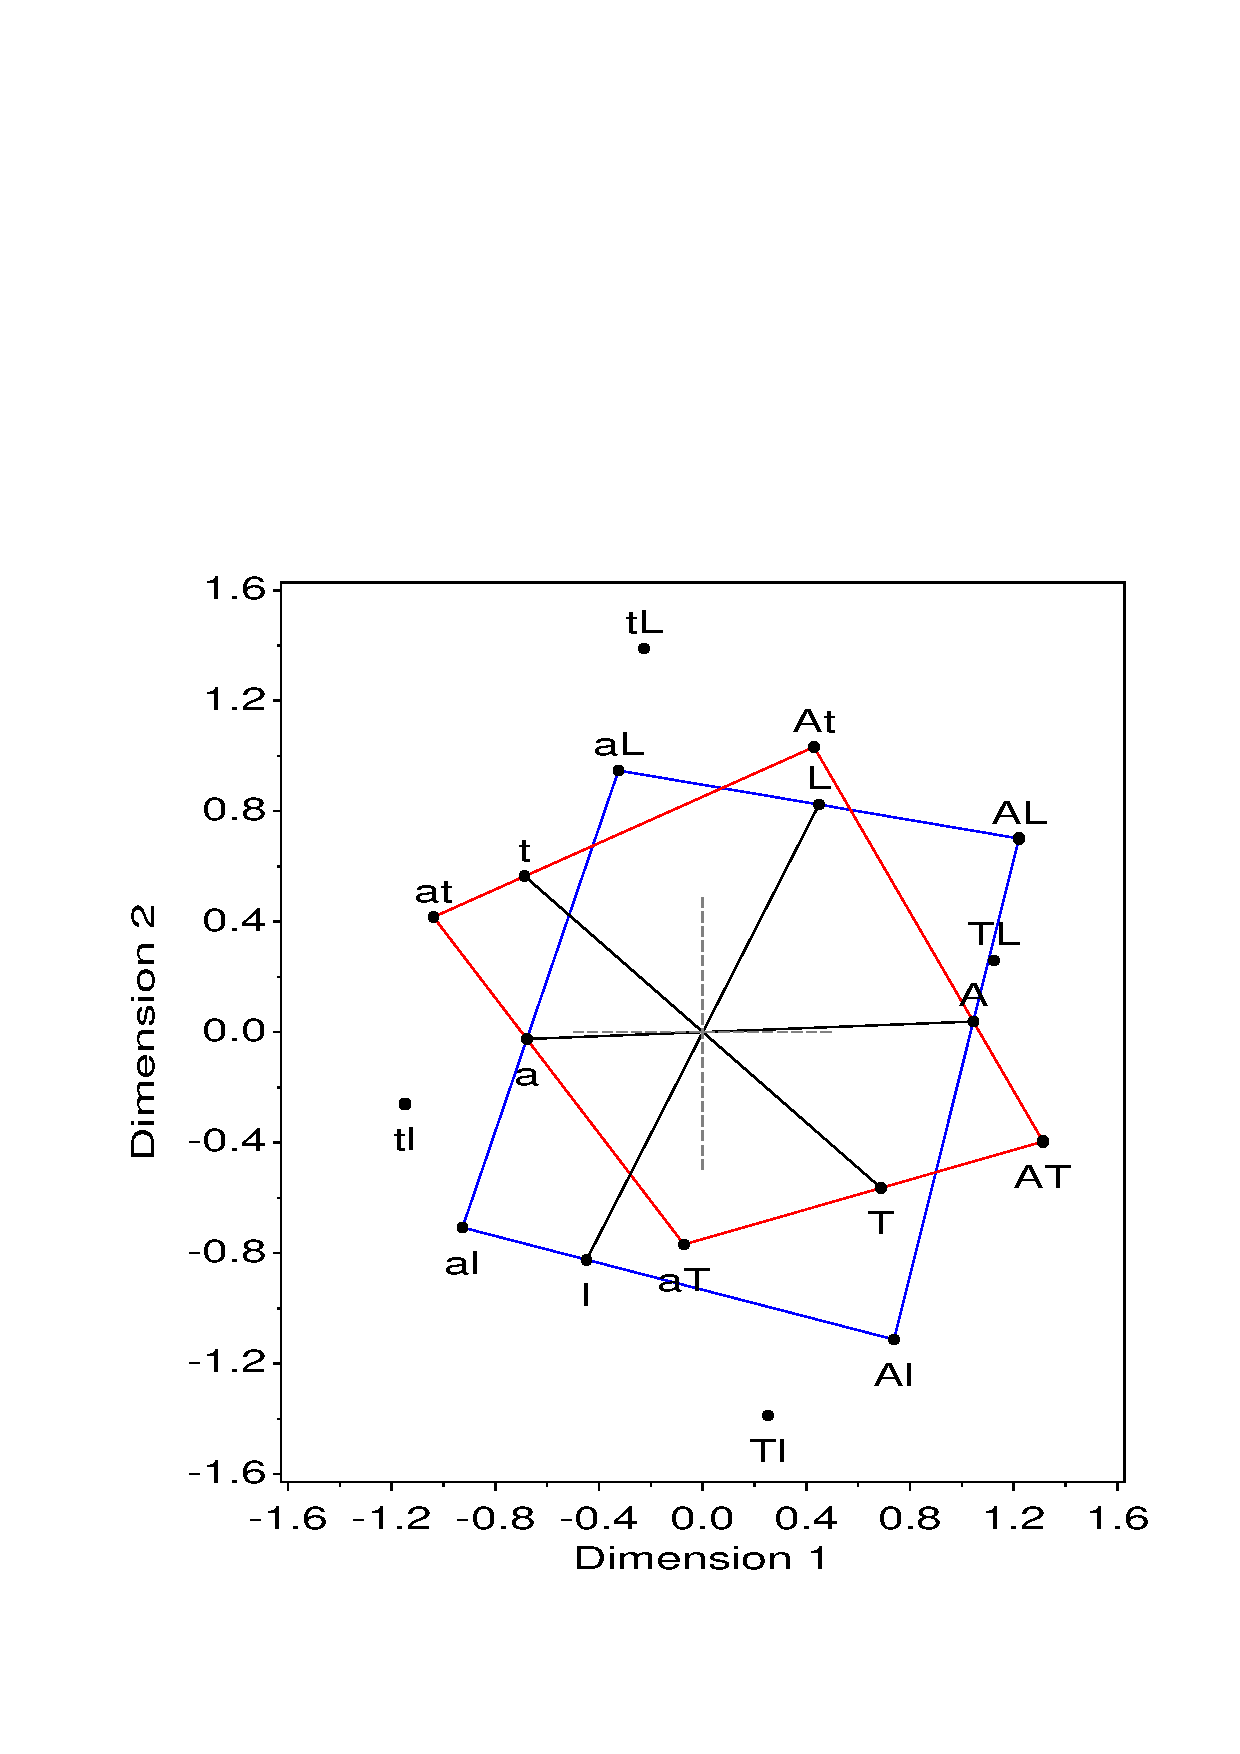
\includegraphics[width=1\linewidth]{ch5/fig/mcabart3}
 \end{minipage}
 \caption[2D Interaction display for Bartlett's data]{2D Interaction display for Bartlett's data.  Both panels show the same 2D solution for the MCA analysis including pairwise interaction effects.  In the left panel, points corresponding to the TL association are connected; lines joining the one-way
points are parallel to the sides, showing independence.
In the right panel, points for both the AT and AL associations are connected.}\label{fig:mcabart2}
\end{figure}
The following steps construct an \ADS\ to draw a quadrilateral for
each of the AT, AL and TL effects.
To do this, it is necessary to extract the \pname{DIM1} and \pname{DIM2}
of the four points for each effect and transpose these to a single
observation with variables \pname{X1-X4} and \pname{Y1-Y4} respectively.
The \Dset\ \pname{QUADS} created here is shown in \outref{out:mcabart4}
%% input: /users/faculty/friendly/sasuser/catdata/mcabart.sas
%% last modified: 16-Aug-98 12:31
\begin{listing}
*-- Extract x,y coordinates of two-way effects;
proc transpose data=coords(drop=_name_) out=quadx prefix=x;
   where (terms=2);
   var dim1;
   by effect;
proc transpose data=coords(drop=_name_) out=quady prefix=y;
   where (terms=2);
   var dim2;
   by effect;
data quads;
   merge quadx quady;
   drop _name_ _label_;
proc print data=quads;
   format _numeric_ 5.2;
   var x1 y1 x2 y2 x3 y3 x4 y4;
   id effect;

*-- Draw quadrilaterals, connecting points in order 1, 2, 4, 3;
data quads;
   set quads;
   drop x1-x4 y1-y4 i;
   retain xsys ysys '2';
   array xx\{*\} x1 x2 x4 x3;;
   array yy\{*\} y1 y2 y4 y3;
   color = scan('blue red green', _n_);
   do i=1 to 4;
      x = xx[i];  y=yy[i];
      if i=1 then function='poly    ';
             else function='polycont';
      output;
      end;

\end{listing}

\begin{Output}[htb]
\caption{\Dset\ \pname{QUADS}, containing the coordinates of the quadrilateral for each two-way effect}\label{out:mcabart4}
\begin{output}
   EFFECT     X1     Y1     X2     Y2     X3     Y3     X4     Y4

     AL     1.22   0.70   0.74  -1.11  -0.32   0.95  -0.93  -0.71
     AT     1.31  -0.40   0.43   1.03  -0.07  -0.77  -1.04   0.42
     TL     1.12   0.26   0.25  -1.39  -0.23   1.39  -1.15  -0.26
\end{output}
\end{Output}
The steps below complete the custom programming to display the TL
effect, with point labels and vectors for the main effects, in the left panel of \figref{fig:mcabart2}.
%% input: /users/faculty/friendly/sasuser/catdata/mcabart.sas
%% last modified: 16-Aug-98 12:31
\begin{listing}
%label(data=coords, out=label, x=dim1, y=dim2, text=_name_, pos=-);

data lines;
   set coords end=eof;;
   by terms effect notsorted;
   drop dim1 dim2 quality mass;
   x = dim1;
   y = dim2;
   xsys = '2'; ysys='2';

   if terms = 1  then do;
   color = 'black';
   if mod(_n_,2) = 1
      then do; function='MOVE    '; output; end;
      else do; function='DRAW    '; output; end;
   end;   

   if eof then do;
      color='gray'; line=3;
      x=-.5;  y=0;   function='MOVE';  output;   
      x=+.5;  y=0;   function='DRAW';  output;   
      x= 0 ;  y=-.5; function='MOVE';  output;   
      x= 0 ;  y=+.5; function='DRAW';  output;
      end;   
run;

*-- Show the Time X Length effect;
data anotes;
   set label lines quads(where=(effect in ('TL')));

proc gplot data=coords;
   plot dim2 * dim1 
      / frame vaxis=axis1 haxis=axis2 hm=1 vm=1
      anno=anotes;
   symbol1 v=dot h=1;
   axis1  length=6in order=(-1.6 to 1.6 by .4) label=(a=90);
   axis2  length=6in order=(-1.6 to 1.6 by .4);
run;
\end{listing}

The right panel of \figref{fig:mcabart2} is produced
using the same \PROC{GPLOT} step,
but the \ADS\ \pname{ANOTES} is assembled using just the
lines to connect the AT and AL points:
\begin{listing}
*-- Show effects on Alive;
data anotes;
   set label lines quads(where=(effect in ('AL' 'AT')));
proc gplot data=coords;
   ...
\end{listing}

Thus, we see that independence of Time and Length (by design of the
data collection) is characterized by a parallelogram shape for the
two-way points, and by lines joining the A and T one-way points
being parallel to those connecting the two-way points.
Note also that the one-way points are in essentially the same positions
as in \figref{fig:mcabart1}.
The quadrilaterals for the AT and AL effects shown in the right panel
are not quite parallelograms, however;  we could approximate the odds
ratio for each of these effects from the cross-product of distances
as in \eqref{eq:mcainter4}.
Finally, because one of the three quadrilaterals shows parallelism,
we conclude from \figref{fig:mcabart2} that the conditional independence
model, [AT][AL], holds.

An alternative representation allows us to show the cells instead, corresponding
to the ATL terms which were not displayed in \figref{fig:mcabart2}.
\begin{figure}[htb]
  \centering
  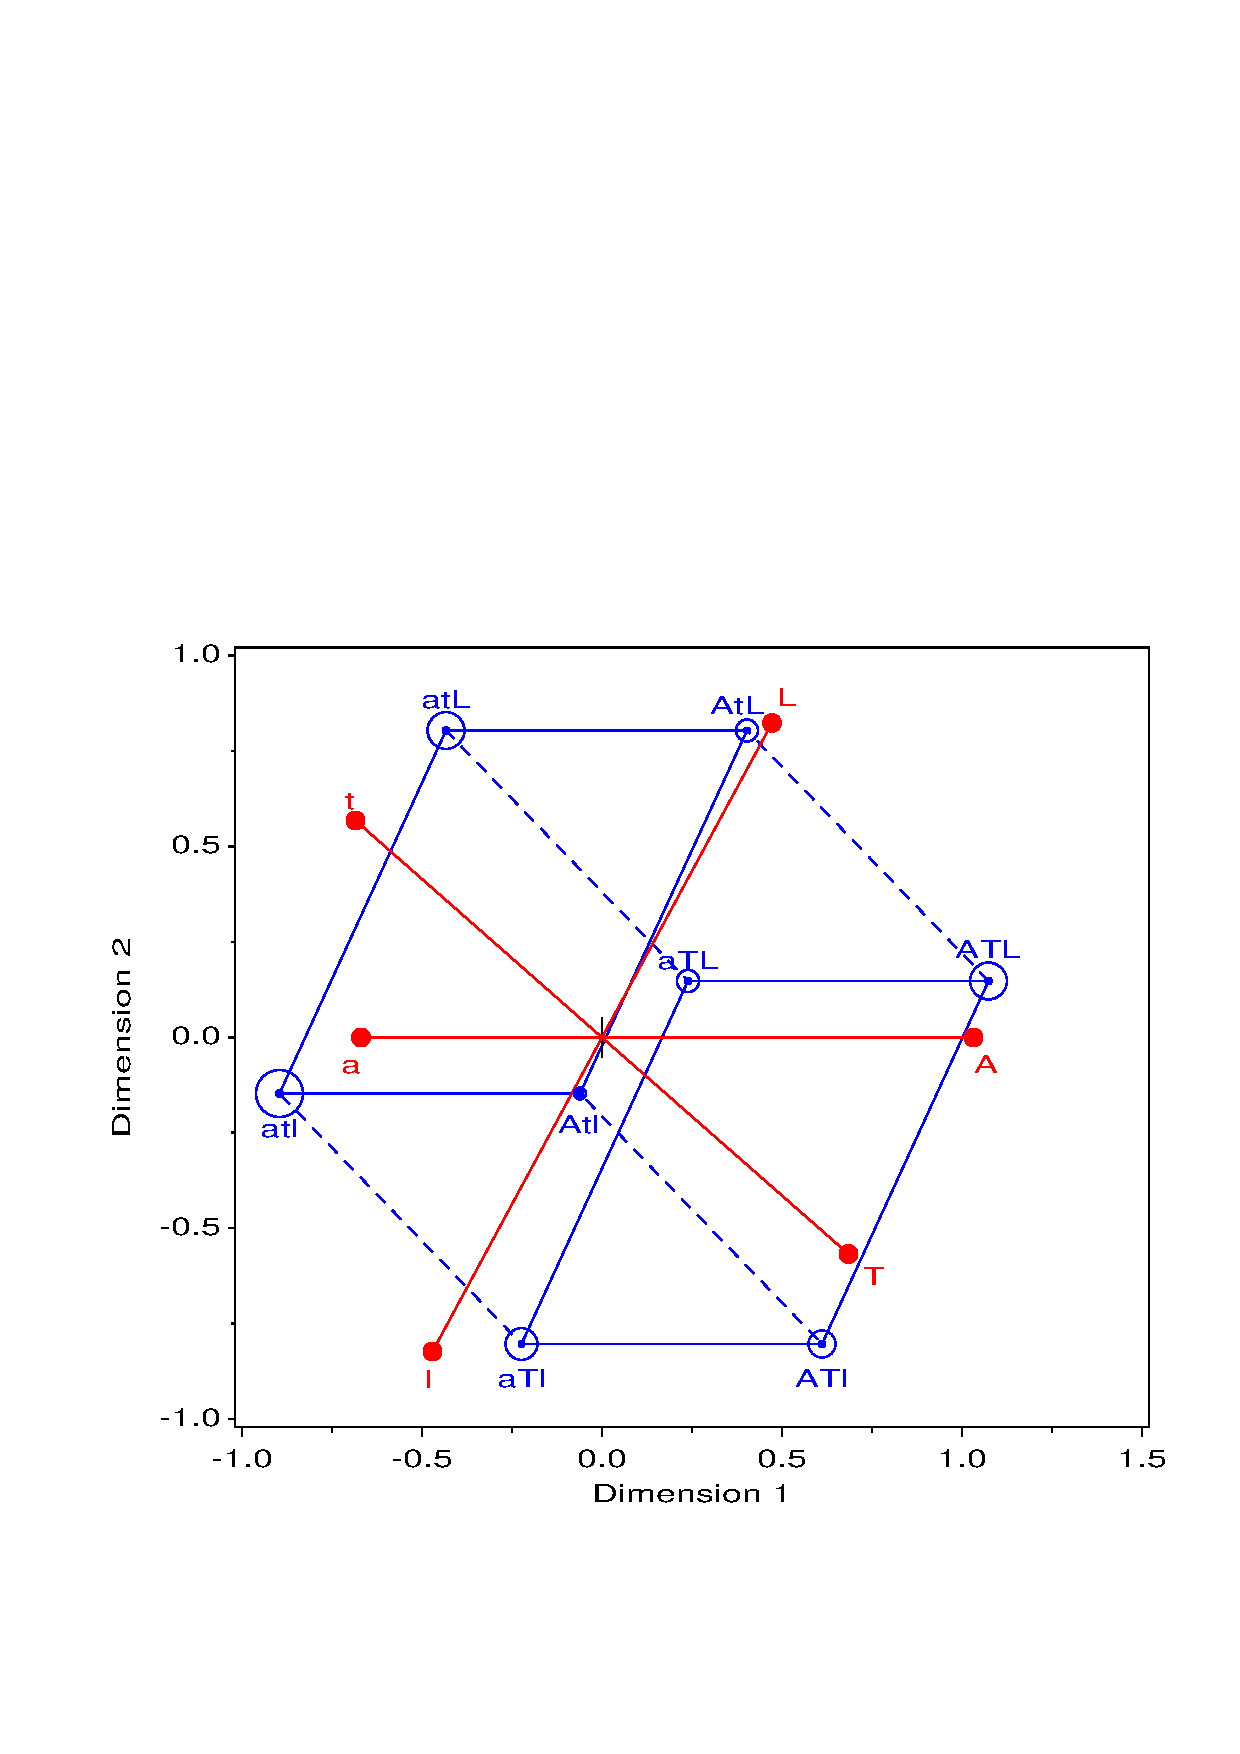
\includegraphics[scale=.7,clip]{ch5/fig/mcagen1}
  \caption[2D representation of the cell points in the $2\times 2 \times 2$ design]{2D representation of the cell points in the $2\times 2 \times 2$ design.  The mass (cell proportion) of each point is shown by the size of the circle.}\label{fig:mcagen1}
\end{figure}
We form the indicator matrix for the main effects,
$\mat{Z} = [
 \mat{Z}_A  \mat{Z}_T  \mat{Z}_L ]$,
and multiply by a diagonal matrix of the cell frequencies, to give:
\begin{output}
   ID    ALIVE   TIME     LENGTH   COUNT    A1    A2    T1    T2    L1    L2

   ATL   Alive   Now      Long      156    156     0   156     0   156     0
   aTL   Dead    Now      Long       84      0    84    84     0    84     0
   AtL   Alive   Spring   Long       84     84     0     0    84    84     0
   atL   Dead    Spring   Long      156      0   156     0   156   156     0
   ATl   Alive   Now      Short     107    107     0   107     0     0   107
   aTl   Dead    Now      Short     133      0   133   133     0     0   133
   Atl   Alive   Spring   Short      31     31     0     0    31     0    31
   atl   Dead    Spring   Short     209      0   209     0   209     0   209
\end{output}
Then, a simple \CA\ of the variables \pname{A1--L2} will have row points
corresponding to the cells, and column for the main effects which are
nearly identical to those from the extended MCA.
This analysis produces the display in \figref{fig:mcagen1}
(program steps are not shown to conserve space), where the
size of the circle at each point represents the mass ($p_{ijk}$) of each
cell, whose label is the \pname{ID} variable above.
The two-way points can be added to this representation by including the two-way indicator matrices, so we analyze the matrix
$\diag (\vec{n}) [
 \mat{Z}_A  \mat{Z}_T  \mat{Z}_L  \mat{Z}_{AT}
 \mat{Z}_{AL}  \mat{Z}_{TL}
]$.
\end{Example}
\ixoff{multiple correspondence analysis!extended}


\ixoff{correspondence analysis!multiple}
\ixoff{correspondence analysis!multi-way tables}
\ixoff{correspondence analysis}
\section{Biplots for contingency tables}\label{sec:biplot}
\ixon{biplot}
Like \CA, the biplot
\citep{BraduGabriel:78,Gabriel:71,Gabriel:80,Gabriel:81}
is a visualization method
which uses the SVD to display a matrix in a low-dimensional
(usually 2-dimensional) space.
They differ in the relationships in the data which are portrayed,
however.
In \CA\ the \emph{distances} between row points and
distances between column points are designed to reflect \emph{differences} between the row profiles
and column profiles.
In the biplot, on the other hand,
row and column points are represented by vectors from the origin
such that the projection 
(inner product) of the vector $\vec{a}_i$ for row $i$
on $\vec{b}_j$ for column $j$ approximates the data element
$y_{ij}$,
\begin{equation}\label{eq:biplot1}
 \mat{Y} \approx \mat{A} \mat{B}\trans \iff
 y_{ij} \approx \vec{a}_i \trans \vec{b}_j
 \period
\end{equation}
Geometrically, \eqref{eq:biplot1} may be described as approximating the data value
$\vec{b}_j$ by the projection of the end point of vector $\vec{a}_i$
on $\vec{b}_j$ (and vice-versa).

For quantitative data \citet{BraduGabriel:78} show how the biplot can be used
to diagnose additive relations among rows and columns. For example, when
a two-way table is well-described by a two-factor ANOVA model with no
interaction,
\begin{equation*}%\label{eq:twoway}
y_{ij} = \mu + \alpha_i + \beta_j + \epsilon_{ij}
\end{equation*}
then, the row points, $\vec{a}_i$, and the column points, $\vec{b}_j$,
will fall on two straight lines at right angles to each other in the
biplot.
For a contingency table, the multiplicative relations among
frequencies under independence become additive relations
in terms of log frequency,
and \citet{Gabriel-etal:97} illustrate how biplots of log frequency
can be used to explore associations in two-way and three-way tables.

Several other biplot representations for contingency tables
are described by \citet{Gabriel:95a,Gabriel:95b}, and in a wider
context by \citet{GowerHand:96}.
\citet{Greenacre:93} discusses the relations between biplots and
both CA and MCA, and shows some conditions under which a
\CA\ plot may be interpreted as a biplot.
More general models, with relations to both CA and biplots are
discussed by \citet{Goodman:86,Goodman:91}.

\subsection{Biplots for two-way tables}\label{sec:biplot2}
\ixon{biplot!two-way tables}
For a two-way table, independence
implies that ratios of frequencies should be proportional for any
two rows, $i, i^{\prime}$ and any two columns, $j, j^{\prime}$.
\begin{equation*}
A \perp B \iff \frac{n_{ij}}{n_{i^{\prime} j}} = \frac{n_{ij^{\prime}}}{n_{i^{\prime} j^{\prime}}}
\end{equation*}
Equivalently, the log odds ratio for all such sets of cells should
be zero:
\begin{equation*}
A \perp B \iff \log \theta_{i i^{\prime}, j j^{\prime}} = \log \left( \frac{n_{ij} n_{i^{\prime} j^{\prime}}} {n_{i^{\prime} j}  n_{ij^{\prime}}} \right) = 0
\end{equation*}
Now, if the log frequencies have been
centered by subtracting the grand mean,
\citet{Gabriel-etal:97} show that $\log \theta_{i i^{\prime}, j j^{\prime}}$
is approximated in the biplot (of $\log(n_{ij}) - \overline{ \log(n_{ij}) }$)
\begin{equation*}
\log \theta_{i i^{\prime}, j j^{\prime}} \approx
\vec{a}_i \trans \vec{b}_j - \vec{a}_{i^{\prime}} \trans \vec{b}_j -
\vec{a}_i \trans \vec{b}_{j^{\prime}} + \vec{a}_i \trans \vec{b}_{j^{\prime}}
= ( \vec{a}_i - \vec{a}_{i^{\prime}} )\trans ( \vec{b}_i - \vec{b}_{i^{\prime}} )
\end{equation*}

Therefore, the biplot criterion for independence in a two-way table
is whether \(  ( \vec{a}_i - \vec{a}_{i^{\prime}} )\trans ( \vec{b}_i - \vec{b}_{i^{\prime}} ) \approx 0\) for all pairs of rows, $i, i^{\prime}$,
and all pairs of columns, $j, j^{\prime}$.
But \( ( \vec{a}_i - \vec{a}_{i^{\prime}} ) \) is the vector connecting
$\vec{a}_i$ to $\vec{a}_{i^{\prime}}$ and
 \( ( \vec{b}_j - \vec{b}_{j^{\prime}} ) \) is the vector connecting
$\vec{b}_j$ to $\vec{b}_{j^{\prime}}$, as shown in \figref{fig:bidemo},
and the inner product of any two vectors equals zero \emph{iff} they
are orthogonal.
Hence, this criterion implies that all
lines connecting pairs of row points are orthogonal to lines connecting
pairs of column points, as illustrated in the figure.
\begin{figure}[htb]
  \centering
  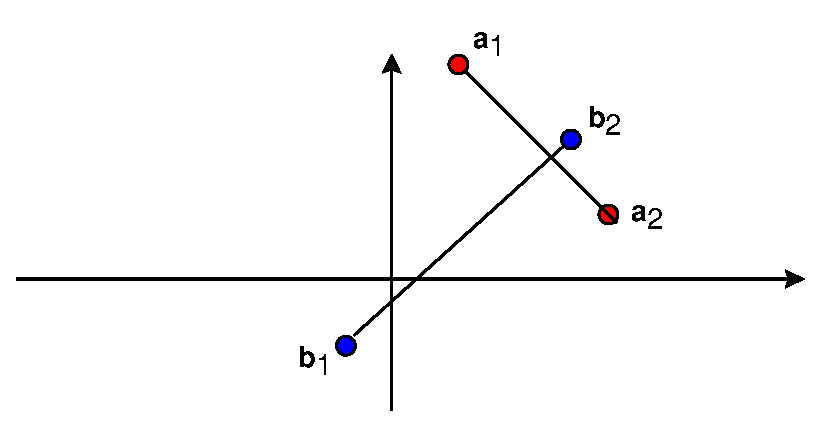
\includegraphics[scale=1]{ch5/fig/bidemo}
  \caption[Independence implies orthogonal vector differences in a biplot of log frequency]{Independence implies orthogonal vector differences in a biplot of log frequency.  The line joining $\vec{a}_1$ to $\vec{a}_2$ represents
 $(\vec{a}_1 - \vec{a}_2)$.  This line is perpendicular to the line
 $(\vec{b}_1 - \vec{b}_2)$ under independence.}  \label{fig:bidemo}
\end{figure}

Thus, when the entire table exhibits independence, the row points
and column points will lie close to two perpendicular lines.
Moreover, a 2-dimensional biplot will account for nearly all of
the variance of the centered log frequencies.
When only a subset of the rows and/or columns are independent,
the points corresponding to those rows and columns will still
lie in orthogonal subspaces, which will be lines or planes
depending on whether a 2D or 3D biplot provides an adequate fit.
An advantage of this method is that it provides a visual indication
of the subsets of rows and columns for which independence does
and does not hold.

\begin{Example}[soccer3]{UK Soccer scores}
We examined the data on UK Soccer scores in \exref{ex:soccer2}
and saw that the number of goals scored by the home and away teams
were largely independent (cf. \figref{fig:soccer2}).
This \Dset\ provides a good test of the ability of the biplot
to diagnose independence.

The biplot analysis is carried out with an enhanced version of
the \macro{BIPLOT} presented in \SSSGref{8,7, A1.2}.
The enhanced version, described in \macref{mac:biplot},
provides automatic equating of the axes
and labeled plots with a variety of interpolation options.

The statements below read the \Dset\ \pname{SOCCER}
and call the \macro{BIPLOT}.  The \mparm{POWER=0}{BIPLOT}
specifies a $\log_{10}$ transformation of the frequencies
contained in the input variables \texttt{A0-A4}.
By default, the \macro{BIPLOT} always standardizes the data
(after transformation, if any) by removing the grand mean,
so the \mparm{STD=NONE}{BIPLOT} indicates no further standardization
is required.
%% input: /users/faculty/friendly/sasuser/catdata/soccer3.sas
%% last modified: 05-Aug-98  9:30
\begin{listing}
title 'UK Soccer scores: Biplot';
data soccer;
   input home $ a0-a4;
datalines;
H0   27 29 10  8  2
H1   59 53 14 12  4
H2   28 32 14 12  4
H3   19 14  7  4  1
H4    7  8 10  2  0
;

%biplot(data=soccer, var=_num_, id=home,
   std=none, power=0,
   out=biplot, anno=bianno,
   symbols=circle dot, interp=none);
\end{listing}


By default, the macro produces a plot of the first two biplot dimensions.
As with the \macro{CORRESP}, the axes are equated in this plot
by default (when the \pname{HAXIS} and \pname{VAXIS} parameters are
not specified).  Sometimes, you may wish
to inspect an initial plot and then
rescale it, as illustrated in \exref{ex:haireye3} and \exref{ex:mental1}.
The macro also produces an \ODS\ of coordinates (\mparm{OUT=BIPLOT}{BIPLOT}) and an \ADS\ (\mparm{ANNO=BIANNO}{BIPLOT}) containing category labels,
which may be used for further customization.

The default plot showed that all of the category points, except for A2 and H2, fell along
separate orthogonal straight lines parallel to the coordinate axes.
The two biplot dimensions account for 99.8\% of the variance.
The statements below are used to find the locations of these lines
from the means of the \pname{DIM1} and \pname{DIM2} coordinates
and append Annotate instructions to draw them to the \pname{BIANNO} \ADS.
The \PROC{GPLOT} step produces \figref{fig:soccer3}.
\begin{figure}[htb]
  \centering
  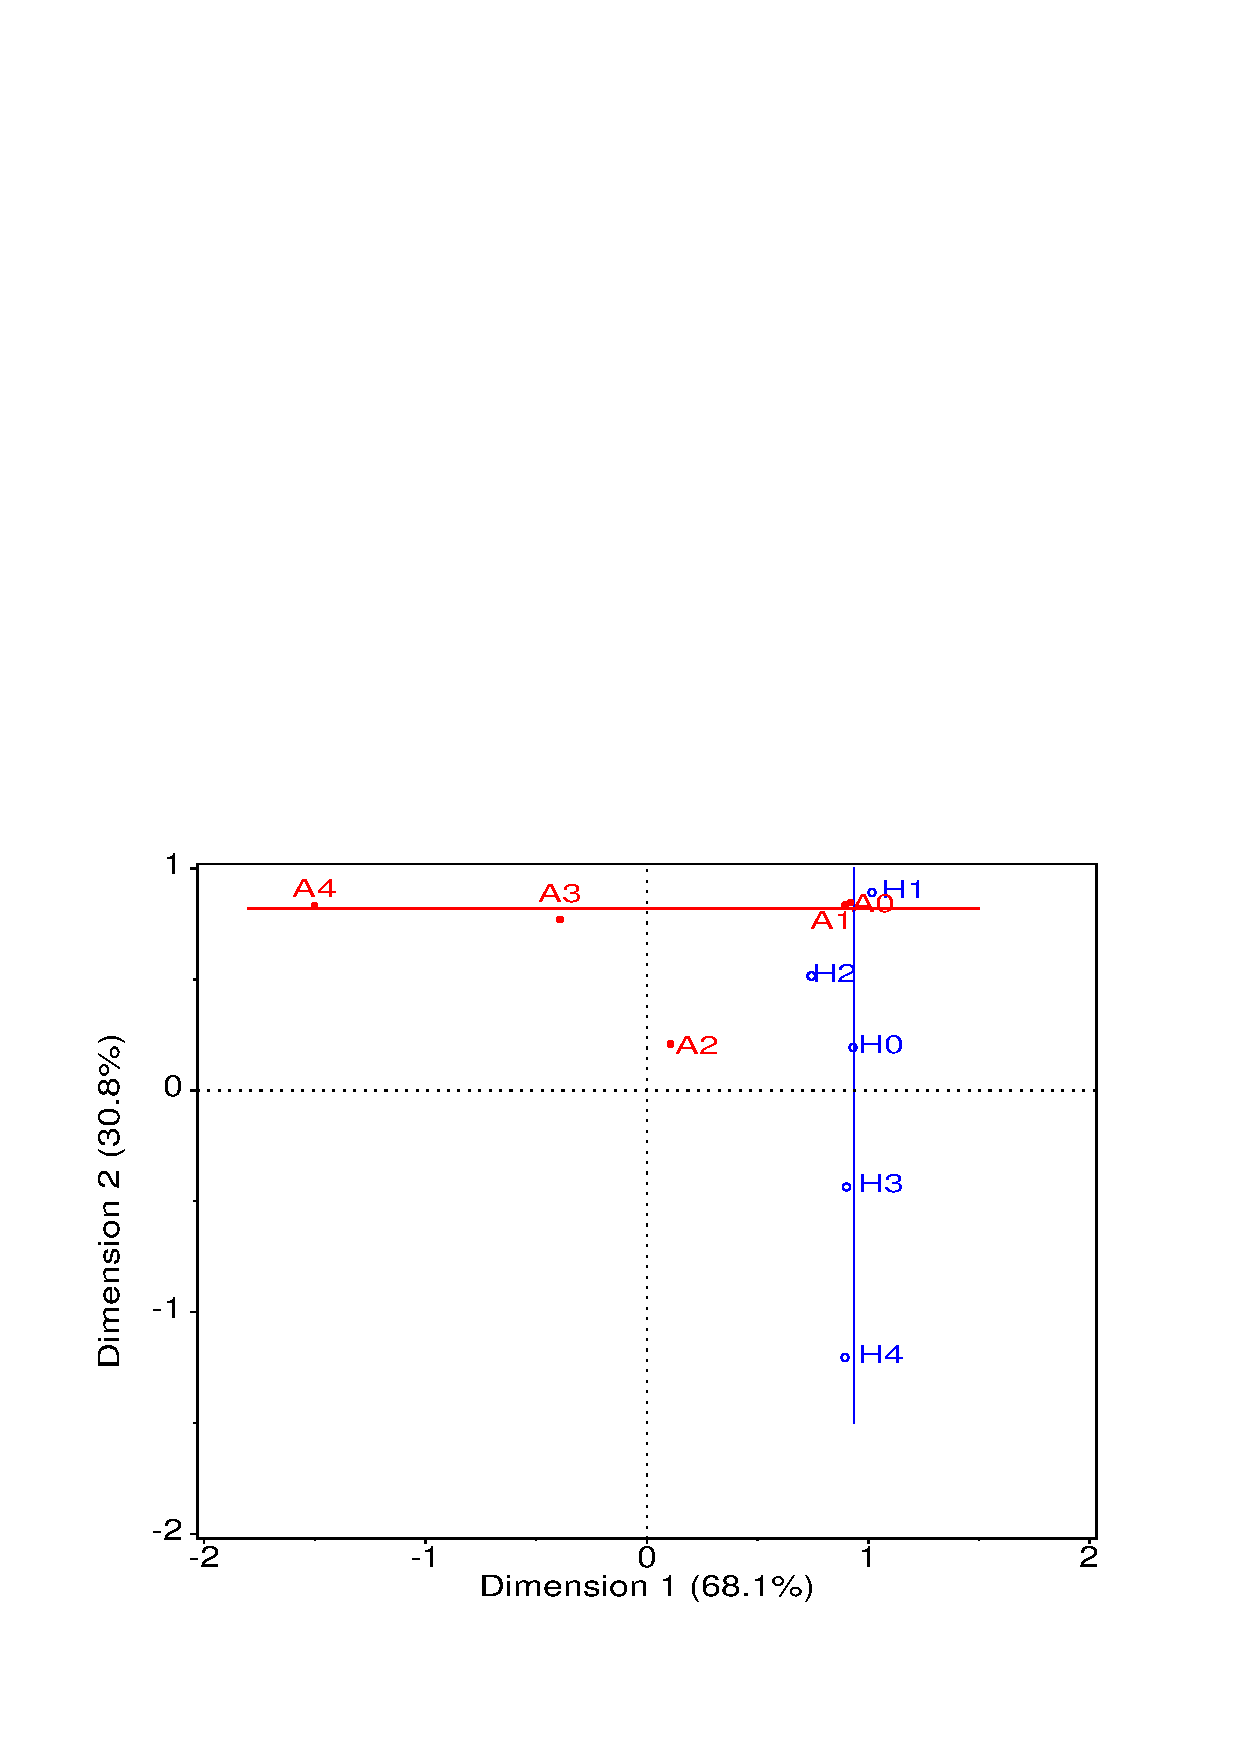
\includegraphics[scale=.6]{ch5/fig/soccer3}
  \caption[Biplot of UK Soccer scores]{Biplot of UK Soccer scores.
  Independence is shown when the row and column points lie on orthogonal
  lines.}  \label{fig:soccer3}
\end{figure}
%% input: /users/faculty/friendly/sasuser/catdata/soccer3.sas
%% last modified: 05-Aug-98  9:30
\begin{listing}
*-- Find mean coordinates (except A2, H2);
proc means data=biplot noprint;
   where (_name_ not in ('A2', 'H2'));
   var dim1 dim2;
   by _type_;
   output out=means mean=;

*-- Draw lines passing thru the means, parallel to axes;
data lines;
   set means;
   xsys='2'; ysys='2';
   length function color $8;
   if _type_ = 'OBS' then do;
      x = dim1; color='blue';
      y = -1.5; function='move';  output;
      y = +1.0; function='draw';  output;
      end;
   else do;
      y = dim2; color='red';
      x = -1.8; function='move';  output;
      x = +1.5; function='draw';  output;
      end;

*-- Append to annotate data set;
data bianno;
   set bianno lines;

title;
proc gplot data=biplot;
   plot dim2 * dim1 = _type_ /
         anno=bianno frame nolegend
         href=0 vref=0 lvref=34 lhref=34
         vaxis=axis1 haxis=axis2
         vminor=1 hminor=1
         name="soccer3" des="Biplot of log(freq)";
      axis1 order=(-2 to 1) length=4.5in label=(a=90) ;
      axis2 order=(-2 to 2) length=6in;
      symbol1 v=circle c=blue i=none;
      symbol2 v=dot    c=red  i=none;
   run;
\end{listing}

We see that all the A points (except for A2) and all the H points (except for H2) lie along straight lines, and these lines are indeed at right angles,
signifying independence.
The fact that these straight lines are parallel to the coordinate axes is
incidental, and unrelated to the independence interpretation.
\end{Example}
\ixoff{biplot!two-way tables}

\subsection{Biplots for three-way tables}
\ixon{biplot!three-way tables}
Biplot displays for three-way tables may be constructed by means of the
``stacking'' approach used in \CA\ described in \secref{sec:ca-multiway}.
That is, a
three-way table,  \(I \times  J \times  K\),
can be represented (in several ways) as a two-way table, with two
variables combined interactively.

As before, consider a three-way $ABC$ table structured as
\(I J \times  K\) so that variables $A$ and $B$ define the rows and
variable $C$ defines the columns.
(Equivalent results obtain for any permutation of the variables.)
Then, a biplot will have row points, $\vec{a}_{ij}$ and column points
$\vec{b}_{k}$ which approximate
\begin{equation*}
\log ( n_{[ij]k} ) - \overline{ \log ( n_{[ij]k} ) }
 \approx \vec{a}_{ij}\trans \vec{b}_{k}
\end{equation*}

By the same arguments of \secref{sec:biplot2},
when $\{A, B\} \perp C$, that is, when the model of joint independence,
$[A B][C]$ holds, then the $\vec{a}_{ij}$ row points will fall on
one straight line and the $\vec{b}_{k}$ will fall on another line,
perpendicular to the first.

Other configurations of points along lines serve as tests for other
models of independence.
For example, if, for a given level $j^{\star}$ of variable $B$, the
points $\vec{a}_{ij^{\star}}$ are collinear and orthogonal
to the line formed by the $\vec{b}_{k}$ of variable $C$,
then \emph{partial independence},
$A \perp C \given B_{j^{\star}}$ holds for level $j^{\star}$.
If this is true for all levels of variable $B$,
then $A$ is conditionally independent of $C$, given $B$,
$\{ A \perp C \} \given B$, or the \loglin\ model $[A B][C B]$.
Thus, for conditional (respectively, partial) independence, the
$\vec{a}_{ij^{\star}}$ points fall on \emph{separate} straight lines
orthogonal to the $\vec{b}_{k}$ for all (respectively, some) levels
of variable $B$, while for joint independence, they all fall on the
\emph{same} straight line.
\ix{biplot!partial independence}
\ix{biplot!conditional independence}
\ix{partial independence!biplot}
\ix{conditional independence!biplot}

Hence, for suitable rearrangement of the variables into a three-way
table, the biplot can be used to identify the major models of
independence.

\begin{Example}[employ2]{Employment status data}
\exref{ex:employ} examined questions of partial and conditional independence
in the Danish employment status data.
We saw (cf. \figref{fig:employp}) that whether a worker was re-employed ($E$)
was independent of length ($L$) of previous employment for those workers
laid off due to closure, but re-employment was strongly associated
for workers who were replaced.

\begin{figure}[htb]
  \centering
  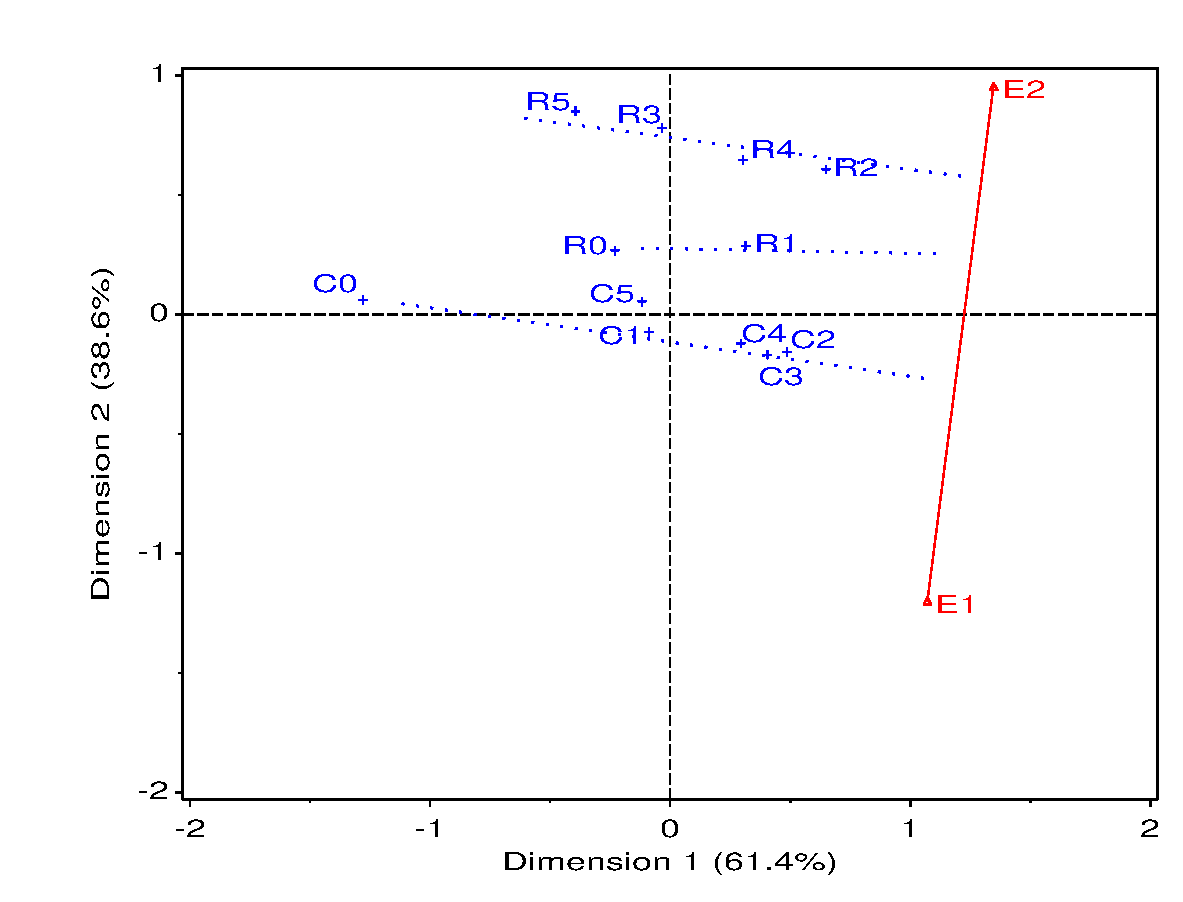
\includegraphics[scale=.8]{ch5/fig/employe}
  \caption[Biplot for Employment status data]{Biplot for Employment status data}  \label{fig:employe}
\end{figure}

The statements below read the data (see \tabref{tab:employ}) in frequency form
and reshape the \pname{COUNT} variable as a $12 \times 2$ matrix
with the variables \pname{CAUSE} and \pname{LENGTH} defining the rows
and the two levels of \pname{EMPLOYED} as columns.
The levels of length of previous employment are identified by the
digits 0 to 6, and the levels of \pname{CAUSE} by `C' (closure) and
`R' (replacement),
which are combined in the \pname{ID} variable for the matrix rows.
The column variables \pname{E1} and \pname{E2} are the two levels
of employment in sorted order, `No' and `Yes'.
%%
%% Table employ written by md2tex 16JUL99 11:22
%%
\begin{table}[htb]
 \caption[Employment Status Data]{Employment Status Data. Employment status on Jan. 1, 1975, by cause of layoff and length of
    previous employment at time of layoff for 1314 employees who lost their
    job in Fall 1974 in Denmark. (Andersen, 1991)}\vspace{5pt}
 \label{tab:employ}
 \begin{center}
  \begin{tabular}{|ll|rrrrrr|}
   \hline
{\bfseries\large Employment} & {\bfseries\large Cause of} & \multicolumn{6}{c|}{\bfseries\large Length of Employment}\rule{0in}{2.5ex}\\
{\bfseries\large Status} & {\bfseries\large Layoff} & $<$1 Mo      & 1-3 Mo     & 3-12 Mo    & 1-2 Yr     & 2-5 Yr     & $>$5 Yr      \\
   \hline
NewJob       & Closure    &    8 &   35 &   70 &   62 &   56 &   38 \\
Unemployed   &            &   10 &   42 &   86 &   80 &   67 &   35 \\
[4pt]
NewJob       & Replaced   &   40 &   85 &  181 &   85 &  118 &   56 \\
Unemployed   &            &   24 &   42 &   41 &   16 &   27 &   10 \\
   \hline
  \end{tabular}
 \end{center}
\end{table}

The call to the \macro{BIPLOT} produces the graph shown in \figref{fig:employe}.
The line joining E1 and E3 was produced by the \mparm{INTERP=NONE JOIN}{BIPLOT}.
The dotted lines were drawn manually (and therefore approximately) in the Graphics Editor.

We see that the points for closure lie approximately along a line perpendicular to the line for E1-E2, indicating partial independence
of employment status
and length for the closure workers (points C0-C5).
The R points for replaced workers do not all fall on one line,
so there is no overall partial independence for these workers;
however, for those workers previously employed for 3 months or more
(R2-R5),  the points are nearly collinear and orthogonal to E1-E2.
\ixoff{biplot!three-way tables}
\ixoff{biplot}
\end{Example}


\section{Chapter summary}
\begin{itemize}
\item Correspondence analysis is an exploratory technique, designed to
show the row and column categories in a two- (or three-) dimensional
space.  These graphical displays, and various extensions, provide
ways to interpret the patterns of association and explore visually
the adequacy of certain \loglin\ models.

\item The scores assigned to the categories of each variable are optimal
in several equivalent ways.
Among other properties,
they maximize the (canonical) correlations between the quantified
variables (weighted by cell frequencies), and make the regressions
of each variable on the other most nearly linear, for each CA dimension.

\item Multi-way tables may be analyzed in several ways.
In the ``stacking'' approach, two or more variables may be combined
interactively in the rows and/or columns of an \nway\ table.
Simple CA of the restructured table reveals associations between
the row and column categories of the restructured table,
but hides associations between the variables combined interactively.
Each way of stacking corresponds to a particular \loglin\ model
for the full table.

\item Multiple \CA\ is a generalization of CA to two or more variables
based on representing the data as an indicator matrix.
The usual MCA provides an analysis of the joint, bivariate relations
between all pairs of variables.

\item An extended form of MCA provides a means to display higher-order
associations among multiple categorical variables.
For $2^Q$ tables composed of $Q$ binary variables, this analysis yields
simple geometric relations that may be interpreted in terms of odds ratios.

\item The biplot is a related technique for visualizing the elements of
a data array by points or vectors in a joint display of their row and
column categories.
An application of the biplot to \ctab\ data is described, based on analysis
of log frequency.
This analysis also serves to diagnose patterns of independence and
partial independence in two-way and larger tables.
\end{itemize}
